%HTTP://inspirehep.net/record/1082936
%
%figures are here:
%https://atlas.web.CERN.ch/Atlas/GROUPS/PHYSICS/PAPERS/STDM-2011-02/

\cmt{
todo:

2010 atlas running 

DQ - in detector chapter?

define coordinates in detector. do rapidity there too.


JP thesis

http://proquest.umi.com/pqdlink?did=1891734781&Fmt=2&VType=PQD&VInst=PROD&RQT=309&VName=PQD&TS=1338239857&clientId=79356
}





\chapter{Inclusive Jet and Dijet Cross-Sections}
\label{INCJETCHAPTER}
\section{Introduction}
\cmt{red To Do: check some things, make sure we understand stuff
choice of scale for dijets - avoids negative cross-sections. These come from negative weights, whats the deal here.

make sure we say why 0.4 and 0.6 are used - sensitivity to pileup/UE effects.

dijets - why different pt cuts for leading and subleading - (easier for theory)
}
%inclusive jet cross-section, any jet in ATLAS. Final result is a double differential cross-section for jet production, binned in rapidity and Jet \pt. Early measurement consisted of $17 nb^{-1}$, covering \pt~from x to x, and rapidity from x to x. In early 2011 the measurement was repeated, using full dataset, increasing the kinematic range covered from x to x. Extending measurement to forward rapidity meant using forward triggers, required knowledge of their behaviour. In addition, trigger scheme for transition region involved some additional complexities. (Discussed in forward trigger Section. )

%
%will first talk about jets in ATLAS and Jet calibration. Then discuss the event selection and data quality used for the analysis. Then talk about TRIGGERS, with emphasis on the forward jet triggers. Data correction talks about unfolding, then discuss results and uncertainties.
The inclusive jet cross-section refers to the cross-section for jet production with no discrimination based on the final state, i.e. all jets in each event are considered. The cross-section measurement is binned in terms of the transverse momentum, \pt, and the jet rapidity, $y$. The cross-sections studied in this chapter are significant as they represent a precise measurement of QCD in a region of phase space that has not previously been explored\footnote{The inclusive jet cross-section measurement made by CDF covers $|y| < 2.1$ and in jet rapidity and 62~GeV~$ < \pt < $~700~GeV in jet \pt~\cite{CDF_incjets}.}. Because QCD is the dominant process at the LHC, the inclusive jet and dijet cross-sections also allow jet production to be properly understood as a source of background in searches for more exotic processes, such as those presented in \cite{monojets,dijets}.
% The jet rapidity is given by
%\begin{equation}
%y = \frac{1}{2} \log \frac{E +p_z}{E - p_z}, 
%\end{equation}
%which reduces to the pseudorapidity in the limit where the jet is massless.% defined rapidity in detector chapter

The first \atlas measurement of the inclusive jet and dijet cross-sections was made in 2010 \cite{InclusivePaperAtlas1,inclusive_confnote_1}, using $17\mathrm{nb}^{-1}$ of early data collected from 7 TeV collisions. The jet production cross-section was measured for jets with \pt~from 60 to 600 GeV and with rapidities less than 2.8 in magnitude. This measurement was updated in early 2011 using the full 2010 \atlas dataset ($37\,\mathrm{pb}^{-1}$) to extend those results. This update expanded the kinematic coverage of the measurement to include jets with \pt~from 20 GeV to 1.2 TeV, and the rapidity range was extended into the forward region to include jets with $|y| < 4.4$\footnote{The FCal coverage extends out to $|\eta| < 4.9$, however an upper limit of 4.4 on the rapidity ensures that the jets under consideration were fully contained within the calorimeter}.   Figure~\ref{fig_kinematic_range} shows the kinematic region covered by the initial measurement compared to that described in this analysis. The dijet mass spectrum has also been measured using 2010 data, and the rapidity coverage of this measurement has also been expanded to include the forward region. The results discussed here have been presented as a conference note \cite{IncJetConf} and were published in 2012 \cite{InclusivePaper2010}. The inclusive jet cross-section has also been measured with the CMS detector using two independent analyses for 2010 data; the first of which covers the region $|y| < 3$ and uses  a ``particle flow'' method to reconstruct jets~\cite{CMSincjet}, while the second covers the region $3.2 < |\eta| < 4.7$ and uses jets reconstructed from the CMS forward calorimeter~\cite{CMSincjetForward}. The \atlas measurement of the inclusive jet cross-section discussed in this chapter coherently uses the same jet reconstruction technique throughout the analysis, with no gaps in the rapidity coverage. The dijet mass spectrum has also been measured at CMS, though only for jets in the region $|y| < 2.5$ \cite{CMS_dijet},whereas the \atlas dijet analysis presented here has the same rapidity coverage as the inclusive analysis ($|y| < 4.4$). 

%\cite{CMSincjet,CMSincjetForward},

Section~\ref{sec_2010_overview} gives a brief overview of the operation of \atlas and the LHC during 2010, while Section~\ref{sec::jetsinatlas} describes how jets are defined and calibrated in \atlas data. The event selection and triggers used for data collection are described in Section~\ref{sec::eventselection}, while Section \ref{sec::unfolding} describes the method used to correct for detector resolution effects in the measured data (``unfolding''). The treatment of experimental uncertainties is described in Section~\ref{sec::uncertainties}, and results are presented in Section~\ref{sec::results}. 

%
%
%
%%\red{something about dijets here}
%%
%%\red{mention dijets}
%%\red{theoretical predictions}
%
%%Initial measurement, extension, cross-section binned in terms of rapidity and Jet \pt
%%motivation, probe QCD in new kinematic regime, understanding jet backgrounds in other analyses.
%
%%will talk about Jet Reconstruction in atlas, discussing the anti-kt algorithm used. Also calibrating jets to the et Energy scale and uncertainties associated with this.
%%Will then talk about the trigger strategy used for the analysis. There are some complexities relating to jet triggers in the rapidity region from $2.8 < |y| < 3.6$, referred to as the ``transition bin'', which will be discussed in detailed in Section~\ref{IncJets_transbin}.

\begin{figure}[tbp]
\begin{center}
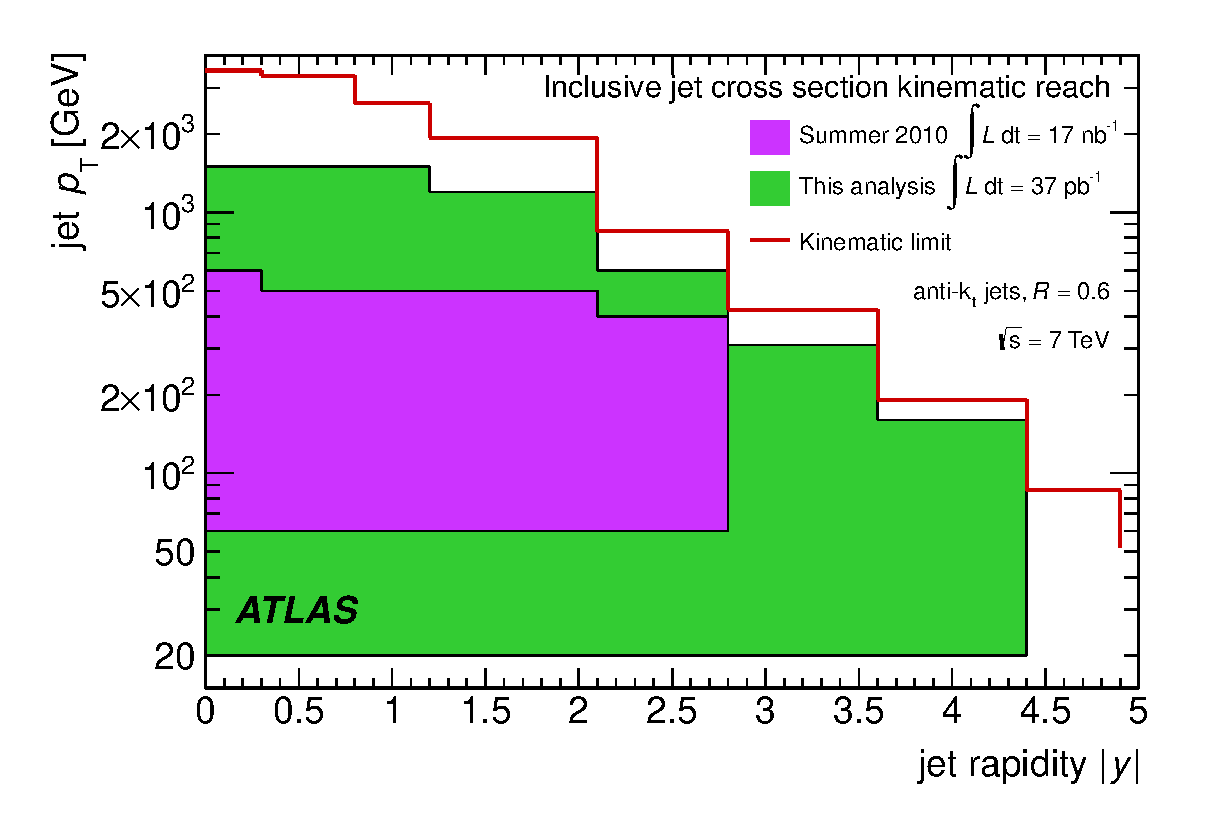
\includegraphics[width=0.8\linewidth,angle=0]{inclusive_results/figs_new/fig_01.eps}%KinematicRange}
\end{center}
%\centerline{\epsfig{file=./figs/collinear.eps  , width=0.95\textwidth}}
\caption[Kinematic range of inclusive jet cross-section measurements]{Diagram showing the kinematic range covered by the first inclusive jet cross-section measurement (purple) using $17\mathrm{nb}^{-1}$ of early data, and that covered when using the full $37\mathrm{pb}^{-1}$ from the 2010 dataset (green).}
\label{fig_kinematic_range}
\end{figure}
\clearpage

\section{Overview of 2010 Running}
\label{sec_2010_overview}
%\red{took x amount of data. nine run periods (a-I), further divided into sub-periods. 2010 was the start of 7 TeV collisions, so systems were commissioned as data taking progressed. luminosity also improved over the course of the year., from XIX to YYY. size of these luminosity increases significant, as a t several points during the year the size of the 2010 was doubled within a single %run of duration $\sim$20 hours.} data taken in lumi blocks. data quality - good detector status


Data taken during 2010 has been divided into nine data periods, A-I. Each period represents an interval during which there were no major changes to the configuration of the detector and trigger, or to that of the LHC.  Each run is subdivided into a number of luminosity blocks (LB), each of which corresponds to $\sim$2 minutes worth of recorded data.
The instantaneous luminosity achieved by the LHC improved over the course of the year as the accelerator was commissioned, from $2 \times 10^{27} \mathrm{cm}^{-2} \mathrm{s}^{-1}$ early in the year to $2 \times 10^{31} \, \mathrm{cm}^{-2}\, \mathrm{s}^{-1}$ by the end of $pp$ running. \cmt{At present (Fall 2012), the LHC is running with an instantaneous luminosity is around $7 \times 10^{33}\, \mathrm{cm}^{-2}\, \mathrm{s}^{-1}$, which slightly less than the design luminosity of $10^{34} \,\mathrm{cm}^{-2} \,\mathrm{s}^{-1}$.}



%The total integrated luminosity recorded by ATLAS from $pp$ collisions in 2010 was 45$\mathrm{nb}^{-1}$. 
%, as can be seen in Figure~\ref{luminosity_fig}. Instantaneous luminosity delivered increased from $2 \times 10^{27}\, \mathrm{cm}^{-2} \,\mathrm{s}^{-1}$ initially to $2 \times 10^{31}\, \mathrm{cm}^{-2} \,\mathrm{s}^{-1}$. 

The amount of data delivered by the LHC and recorded by \atlas throughout 2010 is shown in Figure~\ref{luminosity_fig}. In total \atlas recorded 45 $\mathrm{pb}^{-1}$ of data from $pp$ collisions. Note that this value is slightly lower than the integrated luminosity delivered by the LHC (48.1 $\mathrm{pb}^{-1}$). The Inner Detector contains sensitive electronics, and so is only supplied with high voltage after stable running conditions have been established. This is the main reason for the discrepancy between the amount of data delivered and that recorded.

Certain data quality (DQ) requirements were put in place to ensure that the data used in this analysis was recorded when all relevant systems were functioning correctly. These criteria will be described in detail in Section~\ref{sec::eventselection}.  After imposing these conditions, the analysis is carried out using the remaining 37 $\mathrm{pb}^{-1}$ of data. 

%were all functioning normally. Muons not used, don't care about muons. Because of these DQ requirements, only 37$\mathrm{nb}^{-1}$ of data is used in the analysis.
%
%L1ctp solenoid, inner detector (pixel, sct, trt), calorimeters, luminosity, and tracking, jet, and missing Et reconstruction performance. Also HLT when it was in operation

%lhc stablebeams T
%725 ptag data10_7TeV
%726 dq ATLGL LBSUMM#DetStatus-v03-repro05-01 g
%727 dq L1CTP LBSUMM#DetStatus-v03-repro05-01 g
%728 dq L1CAL LBSUMM#DetStatus-v03-repro05-01 g
%729 dq atltor LBSUMM#DetStatus-v03-repro05-01 g
%730 dq atlsol LBSUMM#DetStatus-v03-repro05-01 g
%731 dq pix LBSUMM#DetStatus-v03-repro05-01 g
%732 dq sct LBSUMM#DetStatus-v03-repro05-01 g
%733 dq trtb,trte LBSUMM#DetStatus-v03-repro05-01 g
%734 dq CP_TRACKING LBSUMM#DetStatus-v03-repro05-01 g
%735 dq CP_MET_METCALO LBSUMM#DetStatus-v03-repro05-01 g
%736 dq CP_JET_JETEC LBSUMM#DetStatus-v03-repro05-01 g
%737 dq CP_JET_JETEA LBSUMM#DetStatus-v03-repro05-01 g
%738 dq CP_JET_JETB LBSUMM#DetStatus-v03-repro05-01 g
%739 dq CP_JET_JETFC LBSUMM#DetStatus-v03-repro05-01 g
%740 dq CP_JET_JETFA LBSUMM#DetStatus-v03-repro05-01 g
%741 dq LUMI LBSUMM#DetStatus-v03-repro05-01 g
%742 dq IDBS LBSUMM#DetStatus-v03-repro05-01 y+

% were put in place to ensure that all detectors and triggers relevant to this analysis were functioning properly. 
%
%quality requirements put in place to ensure that the data used in this analysis was recorded when all relevant detectors and triggers were functioning correctly.
%
%
%
%However data quality requirements meant that only 37$\mathrm{nb}^{-1}$ is used for the analysis.




\begin{figure}[tbp]
\begin{center}
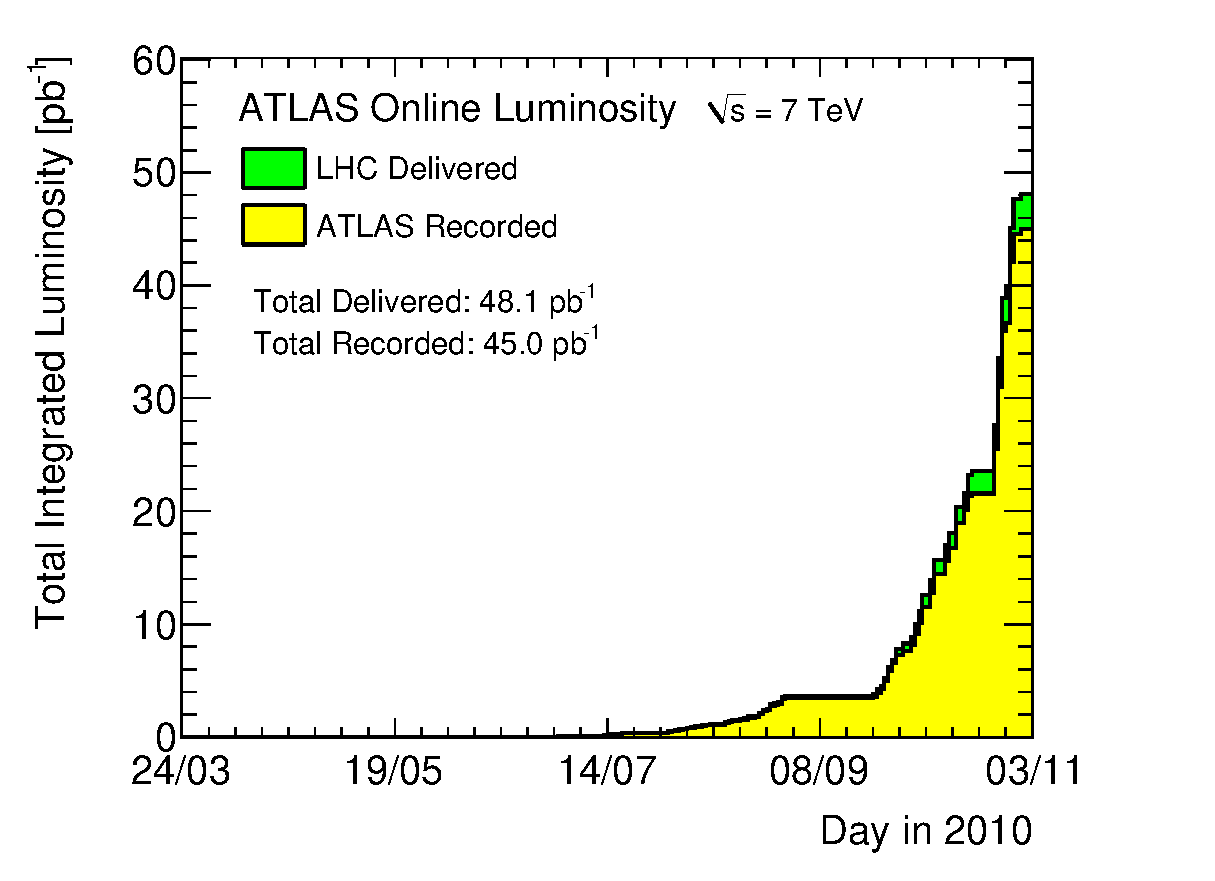
\includegraphics[width=0.8\linewidth,angle=0]{Lumi_2010.eps}
\end{center}
\caption[Integrated luminosity at ATLAS in 2010]{Integrated luminosity recorded by ATLAS over the course of 2010. }
\label{luminosity_fig}
\end{figure}

\section{Jets in ATLAS}
\label{sec::jetsinatlas}
%Jets are built from calorimeter data. 
For the inclusive jet cross-section and dijet analyses, jets were reconstructed using the \akt algorithm running on (EM scale) topological clusters of calorimeter cells. In this Section, jet finding algorithms will be presented, followed by a discussion of the jet calibration method and the uncertainty on the jet energy scale.
%\red{moved topoclusters to FCalTB chap}

\cmt{
\subsection{Topological Clustering}
\label{sec::jetsinatlas_topo}
Topological clusters (or topoclusters)  are formed by grouping neighbouring calorimeter cells based on their signal to noise ratio \cite{Lampl:1099735}. Cluster seeds are found by searching for calorimeter cells that have an energy greater than some multiple, $t_\mathrm{seed}$, of their noise RMS. The noise value used is obtained by adding in quadrature the contributions from electronics noise and pile-up. 

Neighbour cells are then added to the cluster provided they are adjacent to the seed cell and that their signal to noise ratio exceeds the neighbour threshold, $t_\mathrm{neighbour}$. This step is then repeated, with additional neighbour cells being added to the cluster if they are adjacent to an existing neighbour cell and their signal to noise ratio exceeds $t_\mathrm{neighbour}$. This is done until no new neighbour cells are found. Finally, boundary or perimeter cells are added to the cluster by taking all cells that are adjacent to neighbour or seed cells and that have a significance greater than $t_\mathrm{cell}$. 

Hadronic clusters use a ``420'' scheme, where $t_\mathrm{seed}$, $t_\mathrm{neighbour}$ and $t_\mathrm{cell}$ have values of 4,2 and 0, respectively. In this case, the signal is defined as the absolute value of the energy deposited in the calorimeter cell when searching for seed and neighbour cells. This ensures that the contribution from noise is handled symmetrically. A high value of $t_\mathrm{seed}$ makes it unlikely that a cluster will be seeded purely from noise, while a  low $t_\mathrm{cell}$  means that low  energy cells around the periphery of the shower are still clustered. A ``633'' scheme is also used in ATLAS to cluster electromagnetic objects, while other schemes have been investigated using testbeam data \cite{LouiseThesis}. Topoclusters created using the 420 scheme are used as inputs for the jet algorithms considered in this analysis.
}


\subsection{Jet Finding Algorithms}
%\red{ Italicize kt??}
\label{incjets_jetfinding}
Jet finding algorithms are run on a set of input objects, which are referred to as constituents. In general any object with an associated four-vector may be used as a constituent; however for this analysis topoclusters (discussed in Section~\ref{FCALTB_topoclusters}) are the only constituents considered\footnote{ Although ``track jets'' are used for some systematic studies and ``truth jets'' are used in the derivation of the jet calibration and in the unfolding. These use tracks and ``truth particles'', respectively, as their constituents, and will be discussed later}. The jets considered in this analysis are reconstructed using the \akt algorithm \cite{Cacciari:2008gp}. The family of \kt-like jet algorithms operate by forming a list of all the constituents in the event. For all constituents and pairs of constituents, the jet resolution quantities 
\begin{equation}
d_{ij} = \min(k_{ti}^{2p},k_{tj}^{2p}) \frac{(y_i - y_j)^2 + (\phi_i - \phi_j)^2}{R^2}
\end{equation}
and
\begin{equation}
d_i  = k_{ti}^{2p}
\end{equation}
%\end{eqnarray}
are computed, where $k_{ti}$, $\phi_i$ and $y_i$ are the transverse momentum, azimuthal angle and rapidity of the $i$-th constituent, respectively. The distance parameter $R$ is related to the desired size of the jets being found, such that the reconstructed jets will be separated by no less than $R$ in $(y,\phi)$-space. In this analysis, jets with $R =0.4$ and $R=0.6$ are studied. The parameter $p$ defines the jet-finding algorithm: $p=1$ corresponds to the \kt algorithm \cite{Catani1993187}, $p=-1$ gives the \akt algorithm, and $p=0$ corresponds to the Cambridge-Aachen cone algorithm \cite{CA_cone}. %such that found jets will be separated by no less than D in rapidity and azimuth

%\red{we use values of R=04 and R=0.6, WHY??? - larger radius, get more of the QCD radiation, but also more sensitive to underlying event.}

Once the $d_{ij}$ and $d_i$ have been computed, the values are sorted. If the smallest value present corresponds to a $d_{ij}$, then the $i$-th and $j$-th constituents are formed into a proto-jet by summing their four momenta. The proto-jet is then added to the list of constituents and its components are removed. The $d_{ij}$ and $d_i$ values are then recomputed for all remaining constituents and proto-jets. This process is repeated, with each iteration either adding constituents to an existing proto-jet or merging constituents to form a new one. In the case where a $d_i$ value is smaller than any $d_{ij}$ value, this proto-jet is taken as a complete, final jet and is removed from the list. The process continues until the constituent list is empty, with all constituents having been used to form complete jets. The four momentum of a jet is obtained by summing the four momenta of its constituents. A jet mass may then be defined by calculating the invariant mass of the jet's four momentum.


%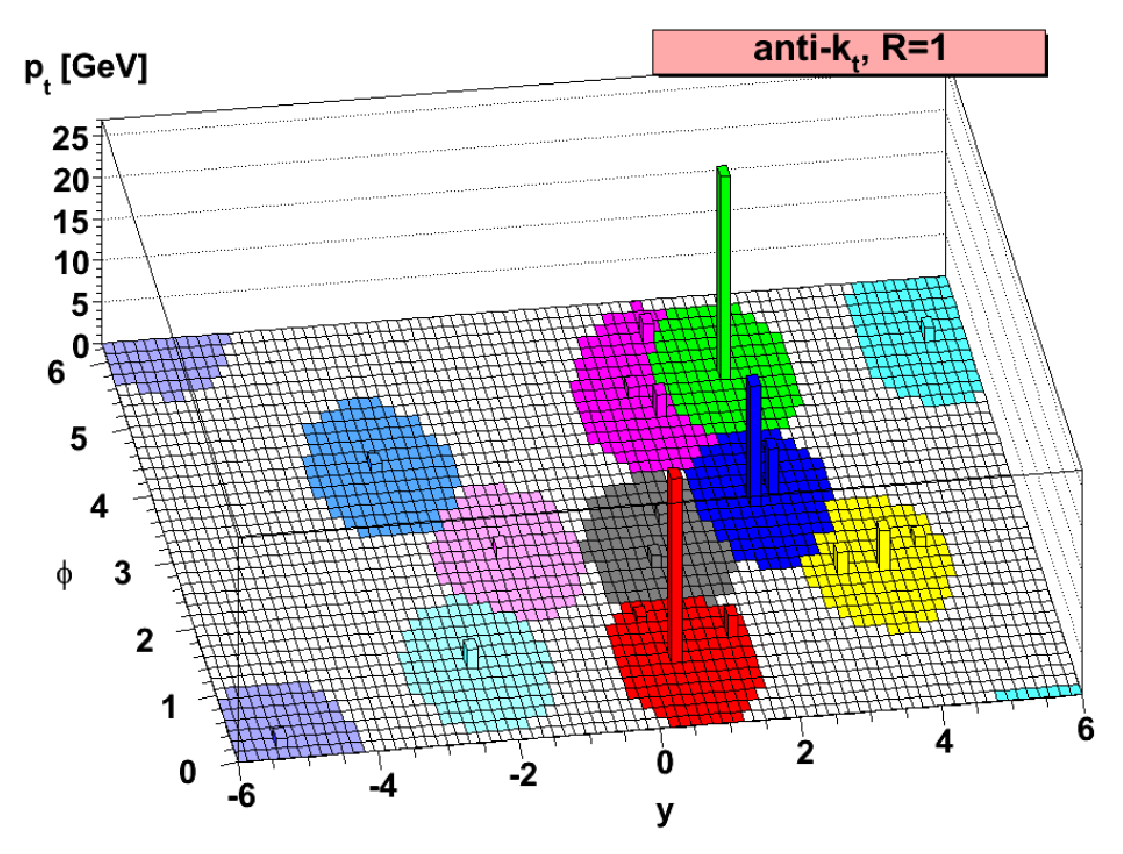
\includegraphics[scale=1]{./figs/akt_finding.eps}
%\includegraphics[scale=1]{./figs/kt_finding.eps}
%\epsfig{file=./figs/akt_finding.pdf}
\begin{figure}[hbt]
\begin{centering}
\subfigure[]{
\includegraphics[width=0.4\linewidth,angle=0]{kt_finding}
\label{fig_ktfinding}
}
\subfigure[]{
\includegraphics[width=0.4\linewidth,angle=0]{akt_finding}
\label{fig_aktfinding}
}
\caption[Comparison of \kt and \akt jet finding algorithms]{Jets found by the \kt algorithm (a) and the \akt algorithm (b). The event was generated using HERWIG \cite{Herwig}, and contains some soft radiation in addition to the high-\pt~constituents\cite{Cacciari:2008gp}.} 
%\label{fig_ktfinding}
\end{centering}
\end{figure}

In the \kt algorithm, $d_{ij}$ is approximately equal to the relative difference in transverse momentum between the two constituents $i$ and $j$, in the limit where the angle between them is small. The \kt algorithm thus clusters together constituents with similar momenta. As showering partons tend to radiate collinearly, the \kt algorithm thus acts to collect all of these radiated constituents and recombine them into a single jet. However, this procedure clusters constituents with the smallest transverse momenta first, such that high \pt~constituents may be clustered around groups of low \pt~constituents. This results in jets with irregularly shaped boundaries, as shown in Figure~\ref{fig_ktfinding}. Conversely, the \akt algorithm considers the highest \pt~constituents first and builds the proto-jets around those, resulting in conically-shaped jets (as shown in Figure~\ref{fig_aktfinding}). This also means that jets found by the \akt algorithm tend to be less sensitive to the effects of pile-up and the underlying event\cite{Cacciari:2008gp}, as the jet is first built around high \pt~constituents and the low \pt~constituents are added to it later, whereas the \kt algorithm would do the opposite.

%
%kt gathers things with similar transverse momenta, undoes QCD hadronisation/branching
%
%deals with smallest differences first. Clusters high \pt~constituents around (groups of) low ones. can give irregularly shaped jet boundaries.
%
%anti-kt similar behaviour to \kt, but clusters big things first, then adds small things to them. Produces very nice, cone shaped jets. Also tends to be insensitive to pile-up and underlying event effects.
\begin{figure}[tbp]
%\label{ir_fig}
%\includegraphics[scale=1]{./figs/ir_safety.eps}

%\centerline{\epsfig{file=./figs/ir_safety.eps  , width=0.95\textwidth}}
\begin{center}
\includegraphics[width=0.8\linewidth,angle=0]{ir_safety}
\end{center}
\caption[IR safety in jet finding algorithms]{Illustration of a jet algorithm which is not IR safe. In the Figure on the left, two distinct jets are found around the high-\pt~constituents. In the presence of soft radiation (right), the algorithm finds only a single jet.}
\label{fig_irsafety}
\end{figure}

\begin{figure}[tbp]
\begin{center}
\includegraphics[width=0.8\linewidth, height=0.3\linewidth]{collinear}
\end{center}
%\centerline{\epsfig{file=./figs/collinear.eps  , width=0.95\textwidth}}
\caption[Collinear safety in jet finding algorithms]{Illustration of an algorithm which is not collinear safe. On the left, a jet is found around a single high-\pt~constituent. On the right, the single constituent is replaced by two constituents, each with half the \pt~of the original. In this case, the algorithm fails to find a jet.}
\label{collinear_fig}
\end{figure}

%\begin{figure}[tbp]
%\begin{center}
%\subfigure[Illustration of a jet algorithm which is not IR safe. In the Figure on the left, two distinct jets are found around the high-pt constituents. In the presence of soft radiation (right), The algorithm finds only a single jet.]{\includegraphics[width=0.8\linewidth,angle=0]{ir_safety}
%\label{fig_irsafety}
%}\\
%\subfigure[Illustration of an algorithm which is not collinear safe. On the left, a jet is found around a single high-pt constituent. On the right, the single constituent is replaced by two constituents, each with half the \pt~of the original. In this case, the algorithm fails to find a jet.]{\includegraphics[width=0.8\linewidth, height=0.3\linewidth]{collinear}
%\label{collinear_fig}
%}
%\end{center}
%\end{figure}


The \kt-like jet algorithms are favored because they are both infrared (IR) and collinear safe. IR safety means that the jets found are stable with respect to the presence of low \pt~constituents arising from pile-up or the underlying event.  For an algorithm to be IR safe,  the presence of soft particles can not ``confuse'' the algorithm into mistaking two separate jets for a single large jet, as illustrated in Figure~\ref{fig_irsafety}. Collinear safety requires that the algorithm will still find a jet if, for instance, a single high-\pt~constituent is replaced by two (or more) close together constituents with lower \pt~(Figure~\ref{collinear_fig}). The \kt-like algorithms have these properties, whereas most iterative cone algorithms (such as those presented in~\cite{cones}) tend not to.


%\begin{figure}[tbp]
%\centerline{\epsfig{file=./eps_4_6_2010/Electron_resolution_4L.eps  , width=0.95\textwidth}}
%\caption{Electron Resolution at 4L }
%\end{figure}


%Anti-kt works by taking list of all constituents, and considering the quantities
%
%\begin{eqnarray}
%d_{ij} &=& \min(k_{ti}^{-2},k_{tj}^{-2}) \frac{(y_i - y_j)^2 + (\phi_i - \phi_j)^2}{R^2}\\
%d_i  &=& k_{ti}^{-2}\\
%\end{eqnarray}
%where $k_{ti}$, $\phi_i$ and $y_i$ are, respectively, the transverse momentum, azimuthal angle and rapidity of the $i$-th constituent, and $R$ is a distance parameter describing the desired size of the jets being sought after. \red{Some motivation for doing this}.


%\begin{figure}[tbp]
%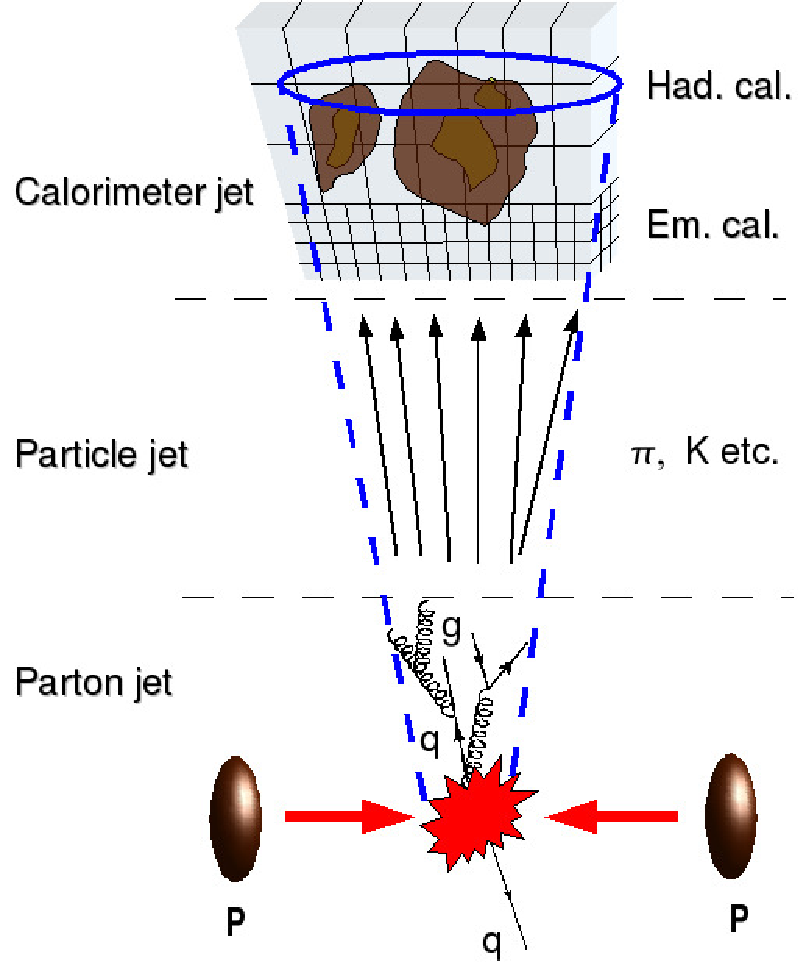
\includegraphics[width=0.8\linewidth,angle=0]{jet_jetsch}
%\end{figure}
%
%\begin{figure}[tbp]
%\centerline{\epsfig{file=./figs/ir_safety.eps  , width=0.95\textwidth}}
%\end{figure}
%
%
%
%\begin{figure}%[ptb]
%  \begin{center}
%    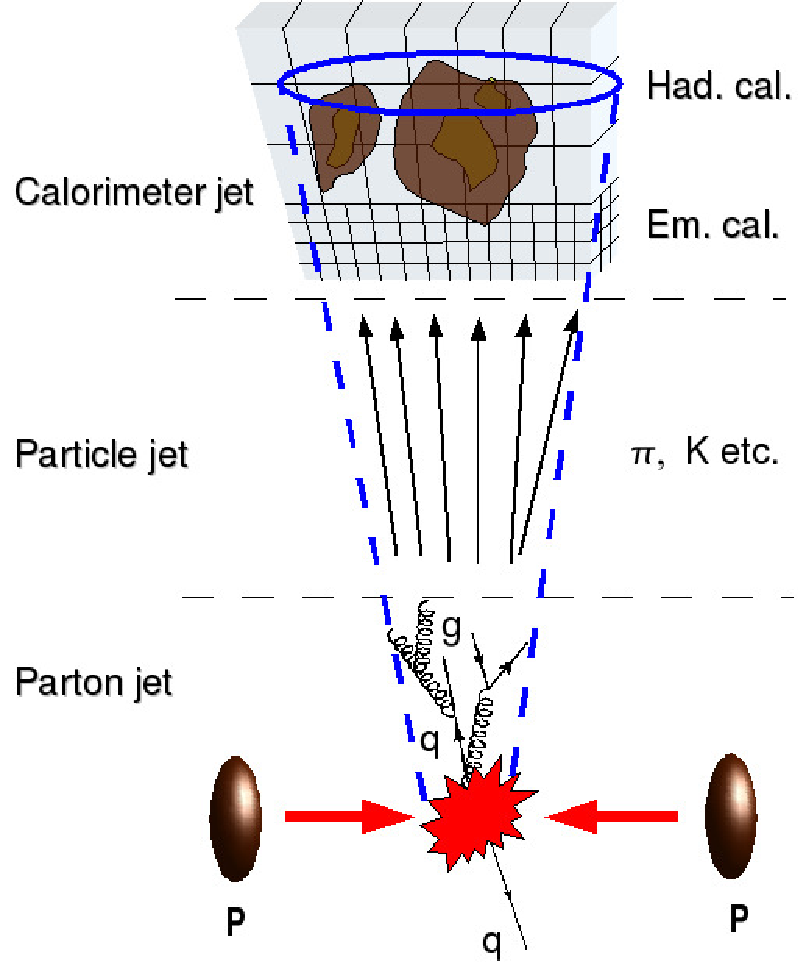
\includegraphics[width=0.8\linewidth]{jet_jetsch}
%  \end{center}
%  \caption[Schematic view of a hard proton-proton interaction]
%          {Schematic view of a hard proton-proton interaction.\label{fig:qcdjet}}
%\end{figure}

\subsection{Jet Energy Scale Calibration}
\label{section_JES}
%
%%\blue{when saying reconstructed, do I mean before or after calibration? be consistent. Also mention why numerical inversion is used.}
%
Once a jet has been reconstructed, its energy must be calibrated to the Jet Energy Scale (JES). For this analysis, this is done  through an ``EM+JES'' scheme~\cite{JES_pub}, whereby the EM scale energy of the jet is multiplied by a calibration factor to obtain the energy at the JES.\cmt{mention EM scale? testbeam = z->ee correction?} The calibration is derived from Monte Carlo simulations using a numerical inversion process. \cmt{The jet finding algorithm is run on the final state particles produced by the event generator to form ``truth jets'', which are then compared to the reconstructed jets in the event. The calibration is chosen to maximise the agreement between the truth jets and the reconstructed jets.} %The JES calibration accounts for the following effects:
%\begin{itemize}
%\item{} \red{corrects for pile up effects.}
%\item{} non-compensation of the calorimeter, i.e. the energy is calibrated to the hadronic scale.
%\item{} energy deposited in inactive (uninstrumented) regions of the detector
%\item{} leakage effects from particle showers not fully contained in the calorimeters
%\item{} particles contained in the truth jet but not in the reco jet
%\item{} energy from showering particles that is not collected by the topoclustering algorithm. (out of cluster corrections).
%\end{itemize}
%\cmt{``Calibration'' corrects for pile up. EM+JES does not, it takes the (pile-up corrected) EM scale energy as input, and outputs the calibrated jet}

The calibration is done in three steps. First, the EM scale energy of the jet is adjusted in order to correct for pile-up effects. Additional proton-proton interactions from the same event can deposit energy in the calorimeter, affecting the energy of the high \pt~objects from the hard scattering. Minimum bias data are used to determine the average energy deposited in the calorimeter as a function of pseudorapidity and the number of primary vertices reconstructed from the event. This information is used to subtract the average EM scale energy added to the jet as a result of pileup.

The second step is to correct the kinematics of the jet, still at the EM scale, based on the location of the hard scattering. Initially, jet kinematics are computed using the geometrical centre of \atlas as the origin of the jet. The luminous region of \atlas has a width of $\sim 40-70 \mu \mathrm{m}$ in the transverse directions and $\sim 22$ mm longitudinally \cite{beamspot_2010}, and it is within this volume that the hard scatterings occur. The vertex with the highest sum of squared transverse momenta from tracks ($\sum p_{\mathrm{T},track}^2$) is taken as the position of the hard scatter, and all jet kinematic quantities ($p_\mathrm{T},y,\phi$, etc.) are recomputed using this vertex as the origin. \cmt{ improves angular resolution, improved \pt~response}

Finally, the JES correction is applied. The correction is derived exclusively from Monte Carlo, using samples generated without the inclusion of pile-up. An event generator is used to simulate a hard parton-parton scattering typical of proton-proton collisions, which outputs a set of final state particles and their four momenta. \geant is then used to simulate the interactions of these particles with the detector. The event is then reconstructed using the same methods that are used for the data: calorimeter cells are reconstructed and used to form topological clusters, on which jet finding algorithms are run. ``Truth'' jets are formed by running the jet finding algorithms on the final state particles output by the event generator. 

The JES calibration accounts for the following effects:
\begin{itemize}
%\item{} \red{corrects for pile up effects.}
\item{} non-compensation of the calorimeter, i.e. the energy is calibrated to the hadronic scale;
\item{} energy deposited in inactive (uninstrumented) regions of the detector, such as cryostat walls or support structures;
\item{} leakage effects from particle showers not fully contained in the calorimeters;
\item{} particles contained in the truth jet but not in the reconstructed jet;
\item{} energy from showering particles that is not collected by the topoclustering algorithm (out of cluster corrections).
\end{itemize}
\cmt{EM+JES is the whole thing. JES is the final step. Offset (pileup) and origin are part of EM JES. the JES part corrects for the above things.}

The calibration is derived by comparing the jets reconstructed from the (simulated) calorimeter information to the truth jets. A reconstructed jet is matched to a truth jet if the distance between them satisfies $\Delta R < 0.3$, where $\Delta R = ( \Delta \eta^2 + \Delta \phi^2 )^{1/2}$.
%  is less than 0.3 in $(y,\phi)$. 
%To avoid mis-matching jets, only isolated jets are matched:
Jets are only considered if they are isolated in order to avoid mis-matching in cases where multiple jets are close together. A reconstructed/truth jet must have no other jets with $p_\mathrm{T,EM} > 7 $GeV within $2.5R$, or it is not used in the derivation of the calibration. 

The matched reconstructed-truth jet pairs are then used to define the response $R$, such that 
\begin{equation}
R = \frac{E_\mathrm{reco}^\mathrm{EM}}{E_\mathrm{truth}},
\end{equation}
where $E_\mathrm{reco}^\mathrm{EM}$ is the EM scale energy of the reconstructed jet and $E_\mathrm{truth}$ is the energy of the truth jet. The response is binned in $E_\mathrm{truth}$ and $\eta_\mathrm{det}$, the pseudorapidity of the reconstructed jet at the EM scale. 
For each $(E_\mathrm{truth},\eta_\mathrm{det})$ bin, the mean reconstructed jet energy, $\langle E_\mathrm{reco}^\mathrm{EM} \rangle$, is found, and a Gaussian fit is used to extract the mean response, $\langle R \rangle$. 

The response is then parameterised as a function of $E_\mathrm{reco}^\mathrm{EM}$ for each $\eta_\mathrm{det}$ bin. 
%This is done
For the $k$-th $\eta_\mathrm{det}$ bin, a fit is performed on the $(\langle E_\mathrm{reco}^\mathrm{EM} \rangle,\langle R \rangle)$ points obtained from each $E_\mathrm{truth}$ bin. The fitted function is of the form

\begin{equation}
F_{\mathrm{calib},k}(E_\mathrm{reco}^\mathrm{EM}) = \sum_{j=0}^{N_\mathrm{max}} a_j \left(\log E_\mathrm{reco}^\mathrm{EM}\right)^j,
\end{equation}
where the $a_j$ are free parameters and $N_\mathrm{max}$ is an integer between 1 and 6, depending on $\eta_\mathrm{det}$.

The correction factor is then found by inverting $F_{\mathrm{calib},k}$, so the final EM+JES energy of a jet lying in the $k$-th $\eta_\mathrm{det}$ bin is given by

\begin{equation}
E_\mathrm{reco}^\mathrm{JES} = \frac{E_\mathrm{reco}^\mathrm{EM}}{F_{\mathrm{calib},k}(E_\mathrm{reco}^\mathrm{EM})}.
\end{equation}




\cmt{

mention this:
The present calibration scheme, EM+JES, calibrates the reconstructed jets using energy and  dependent
correction factors derived from simulated Pythia events.4 To derive the correction factors, particle
jets, reconstructed using the Monte Carlo (MC) event record, are matched with jets reconstructed in the
calorimeter, and the correction is calculated by dividing the true particle jet energy by the EM-scale
energy of the matching calorimeter jet.5 Following this, a small -dependent correction is applied to remove
a bias in the reconstructed  of jets that occurs when jets fall in specific regions of the calorimeter
that have a much lower response than the regions around it. The reason for this bias is that jet directions
are reconstructed using the \pt-weighted sum of the constituents directions. The bias occurs when some
of the constituent particles fall into a crack region with low response, and the jet is pulled toward the
region with the higher response.
 }

%A Gaussian fit is made for each $(E,\eta)$ bin from which the mean response, $\langleR\rangle$ is extracted.  


\cmt{
compare truth and reco
ratio R = Ereco/Etruth, binned in Etruth and ndet (reco)
for each bin, mean response <R> is derived from a Gaussian fit and mean <Ereco> is found. 

for each ndet bin, function F is fit to the (<Ereco>,<R>) points( i.e. 1 point for each Etruth bin)

fit function F has form F(Ereco) = \sum_i^Nmax a_i (\log Ecalo)^i 
Nmax chosen between 1 and 6 to maximise goodness of fit.

Final calibration is then just 1/F, i.e.

E_reco(EM+JES) = E_reco(EM)/F|ndet

}


 



\cmt{ 

 Only isolated jets are considered when deriving the calibration, where a jet is considered isolated if no other jets with Em \pt~above 7GeV lie within $2.5R$, where $R$ is the jet radius. Reconstructed jets are then matched to truth jets

 Only isolated jets are considered when deriving the calibration, If two or more jets with EM scale \pt~above 7GeV lie within 2.5R then they are ignored.

Only isolated jets are used when deriving the calibration, so that jets excluded if another jet lies within 2.5R in y,phiOnly isolated jets are considered, A reconstructed jet and truth jet that are separated by $Delta R < 0.3$ are considered to be matched, provided there are no other . 


Truth jets and reconstructed jets within $\DeltaR < 0.3$ of each other are considered to be matched, provided the jets are isolated. A jet is considered isolated if there are no other jets with an EM scale energy above 7 GeV within 2.5$R$ in ($y,\phi$), where $R$ is the radius used in the jet-finding algorithm.  

Then take the ratio of \pt_reco/PT_truth

Calorimeter Jets?

isolated jets nothing over 7 GeV (EM) within 2.5R
matched DR< 0.3
}




\cmt{

Use EM+JES scheme
start at EM, then apply weight
weight comes from MC (numerical inversion)
EM scale originally derived from testbeam
updated/corrected using z->ee data.


weight accounts for 

calorimeter non-compensation (hadronic scale)
dead material
leakage (particles out the back)
particles in truth jet but not in reco jet (out of cone?)
out of cluster corrections/out of jet corrections? (different from above?)

before weighting is carried out, correction is applied to jet energy at EM scale in order to take into account pile up. This correction is parameterised as a function of the number of primary vertices measured in the event and the pseudorapidity of the jet.



\^
1. correct for pileup
2. correct jet kinematics - rapidity and phi recalculated from primary vertex, rather than centre of ATLAS.
3. Numerical inversion

origin correction improves jet angular resolution - improves \pt~response 


Mention Global Cell weighting/local hadronic weighting?

}




\subsection{JES uncertainty}
\label{JES_uncertainty_section}
The systematic uncertainty on the JES is an important quantity, and one of the dominant sources of uncertainty in the inclusive jet and dijet cross-section analyses. There are several sources that contribute to this uncertainty, outlined below:

\begin{itemize}
\item{\bf Relative calibration of uncertainties between forward and central regions.} Contributions to the JES uncertainty from the sources discussed below have been calculated in the central region, $0.3 < |\eta | < 0.8$. This uncertainty is used as a baseline, and an intercalibration method \cite{ATLAS-CONF-2011-014} is used to extend the estimate of the JES systematic into other pseudorapidity regions. This method uses a \pt~balancing technique applied to dijet events in order to obtain the ratio of the calibrated jet responses in different regions of pseudorapidity. This response was calculated for data and simulation, using several different MC event generators. The RMS of the differences in response between MC and data is then added in quadrature to the baseline uncertainty, yielding the uncertainty in higher pseudorapidity regions.
\item{\bf Uncertainty from the calibration method} The EM+JES method calibrates jets by applying a correction factor to the EM scale energy of the jet. This treats all of the jets constituents equally, i.e. each constituent is effectively scaled by the same calibration factor. Additionally, this same correction factor is used for both the energy and transverse momenta of the jet, which may bias the calibrated \pt~in cases where the calibrated jet mass differs from the mass of the truth jet. The uncertainty arising from the calibration method is estimated by comparing the reconstructed jets at the EM+JES scale to their truth jet counterparts. The responses $\langle R_E \rangle = \langle E_\mathrm{reco}^{EM+JES} / E_{truth} \rangle$ and $\langle R_P \rangle = \langle p_\mathrm{T,reco}^{EM+JES} / p_\mathrm{T,truth} \rangle$ are computed, and binned in terms of $p_\mathrm{T,reco}^{EM+JES}$ and $|\eta|$. Any deviation of $\langle R_E \rangle$ or $\langle R_P \rangle$ from unity suggests that the kinematics of the reconstructed jets after calibration are not equal to those of the truth level jets (this is called ``non-closure'')\cmt{, for the reasons mentioned above}. The estimated uncertainty associated with the calibration method is taken as the largest deviation of $\langle R_E \rangle$ or $\langle R_P \rangle$ from unity, and is found to be less than 1\% for $p_\mathrm{T,reco}^{EM+JES} > 30$ GeV and less than 2\% for 30 GeV $> p_\mathrm{T,reco}^{EM+JES} >$ 20 GeV \cite{ATLAS_JES_2010}.

\item{ \bf Uncertainty from calorimeter response} The contribution to the JES systematic from the uncertainty in the calorimeter response is derived from single particle measurements. The uncertainty in the response to charged hadrons is measured in $E/p$ studies \cite{ATLAS-CONF-2011-028} and in testbeam data \cite{Khramov:1172156}. The simulation framework allows the particles in the truth jet to be associated with the energy they deposit in the calorimeter, and thus the single particle response uncertainties can be propagated to obtain an uncertainty for the response of the jet. When estimating this uncertainty, effects relating to the calorimeter acceptance, charged particles with $E> 400GeV$\footnote{Charged particles at these energies could not be studied in beam tests, and so the uncertainties associated with particularly high energy densities or longitudinal leakage must be estimated.}, and energy deposited by neutral hadrons are also considered. Effects related to the calorimeter response are found to contribute $1.5\% -  4\%$ to the JES systematic uncertainty.

\item{\bf Uncertainty due to noise thresholds in detector simulation} The noise present in the calorimeter electronics can change over time, whereas the noise used in the simulation is fixed when the MC sample is generated. The value of the noise RMS used influences which cells are grouped into topoclusters, and thus contribute energy to the jet. The effect of the noise threshold in the simulation was studied by increasing and decreasing the noise thresholds for the topoclustering algorithm by amounts of 5-10\%. The uncertainty assigned to this effect was found to be negligible for jets with \pt~$>$ 45 GeV, and is estimated as 1\% for jets with momentum in the range 30 GeV $\leq \pt \leq$ 45 GeV. For jets with 20~GeV~$\leq \pt \leq 30$~GeV, the uncertainty was estimated as 1\% (2\%) for jets with radius 0.4 (0.6).

%The noise RMS for each cell was measured from data, and these values were then used to define the noise thresholds when reconstructing topoclusters in the simulation. Using the noise thresholds obtained from data had a similar effect to that seen when increasing the default simulation noise thresholds by 7\%. 
%
%
%The effect of the noise threshold in the simulation was measured by \red{increasing} the noise thresholds for the topoclustering algorithm by amounts of 5-10\%. This influences which cells are grouped into topoclusters, and thus contribute energy to the jet. The uncertainty assigned to this effect was found to be negligible for jets with \pt~$>$ 45 GeV, and is estimated as 1-2\% for jets with lower \pt. \red{down to 20 GeV or 30 GeV?}
%
%re-read this as
%
%use noise RMS from data in simulation, reconstruct jets using this noise threshold for topoclusters
%
%increase noise thresholds by 7\% this has the same effect as using data. Symmetric, raising/lowering by 7\% suggests the effect is symmetric.
%
%
%
%\red{1\% (2\%) for jets with $R$ = 0.4 (0.6) with 20 GeV< \pt~< 30GeV, 1\% for 30 < \pt~< 45 GeV.}

\item{ \bf Effect of additional material in simulation} As the JES calibration is intended to correct for the effects of inactive material, it is sensitive to the material description of the detector in the simulation. The effects of this were estimated by adding additional material to the simulation geometry in several places, and comparing the response obtained with the modified geometry to that obtained using the nominal geometry. 
%The variation of the energy response was found to be within 3\%, while that of the $p_T$ response was within 2\%. 
\item{ \bf MC event generators}
The nominal MC sample used in the derivation of the JES was generated using \pythia, using the AMBT1 tune. Samples were also produced using \alpgen~\cite{alpgen} interfaced with \herwig and \jimmy, and using the Perugia2010 tune for \pythia. The \alpgen sample used the CTEQ6.1 PDF set, and treated parton showering and hadronisation effects differently than the nominal \pythia sample, whereas the Perugia2010 sample provided a different treatment of the underlying event. Deviations between the response obtained from the Perugia2010 and \alpgen+\herwig+\jimmy samples with respect to the nominal \pythia sample were used to estimate the uncertainty arising from the choice of physics models. \cmt{define these in QCD chapter, event generators}

%Pythia with Perugia2010 -> underlying event uncertainty
%
%alpgen+herwig+jimmy with CTEQ6.1 -> parton showering,hadronisation,pdfs 




\end{itemize}

The total JES uncertainty, and its components, are plotted in Figure~\ref{JES_uncertainty_figs} for $R=0.6$ jets. The uncertainty in the calorimeter response is the dominant contribution to the JES uncertainty for jets with \pt~$\geq$ 100 GeV. In the central region ($0.3 < |\eta| < 0.8$), the uncertainties associated with alternative MC generators dominate below 100 GeV, while in other pseudorapidity regions intercalibration effects dominate at low \pt. At high \pt~(near the kinematic limit) the JES uncertainty is around 3-5\% in each rapidity region. The uncertainty associated with jets of radius $R=0.4$ is generally similar to that associated with jets of radius $R=0.6$.

% The dominant contribution to the JES uncertainty for in the central region ($0.3 < |\eta| < 0.8$) is from the uncertainty in the calorimeter response. In other pseudorapidity regions the intercalibration uncertainty dominates at low \pt.
 
 
%\begin{figure}[tbp]
%\begin{centering}
%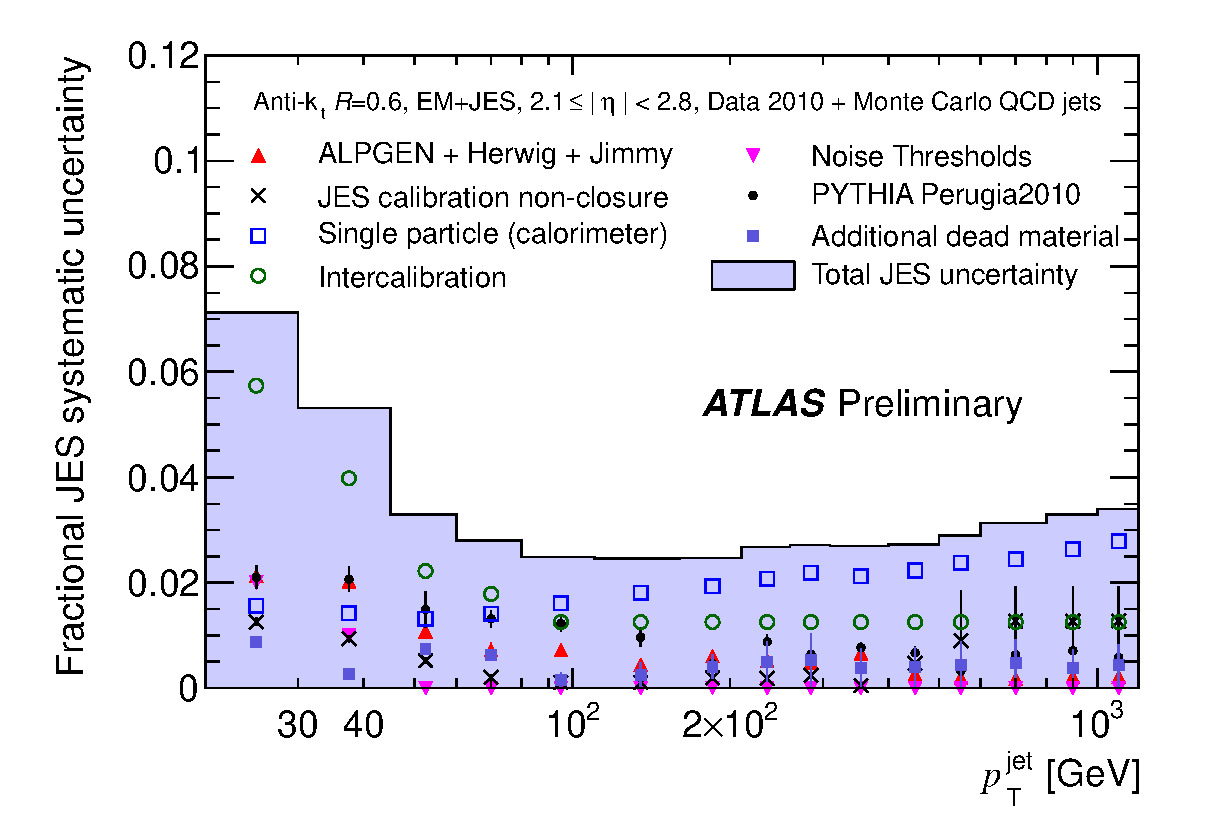
\includegraphics[width=0.45\linewidth,angle=0]{JES_fig_10} 
%\end{centering}
%\caption{}
%\label{JES_uncertainty_1_fig}
%\end{figure}
%
%\begin{figure}[tbp]
%\begin{centering}
%\subfigure{
%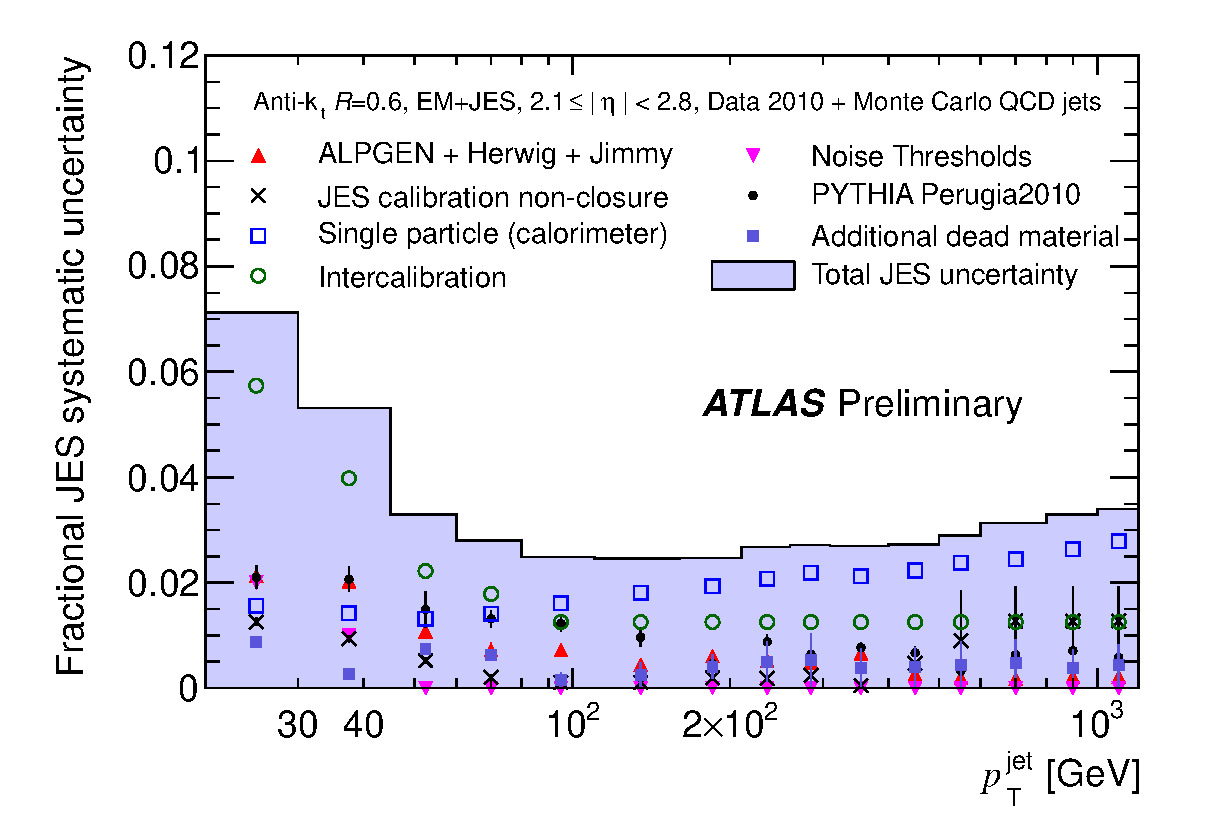
\includegraphics[width=0.45\linewidth,angle=0]{JES_fig_10}
%\label{JES_uncertainty_2_fig}
%}
%\subfigure{
%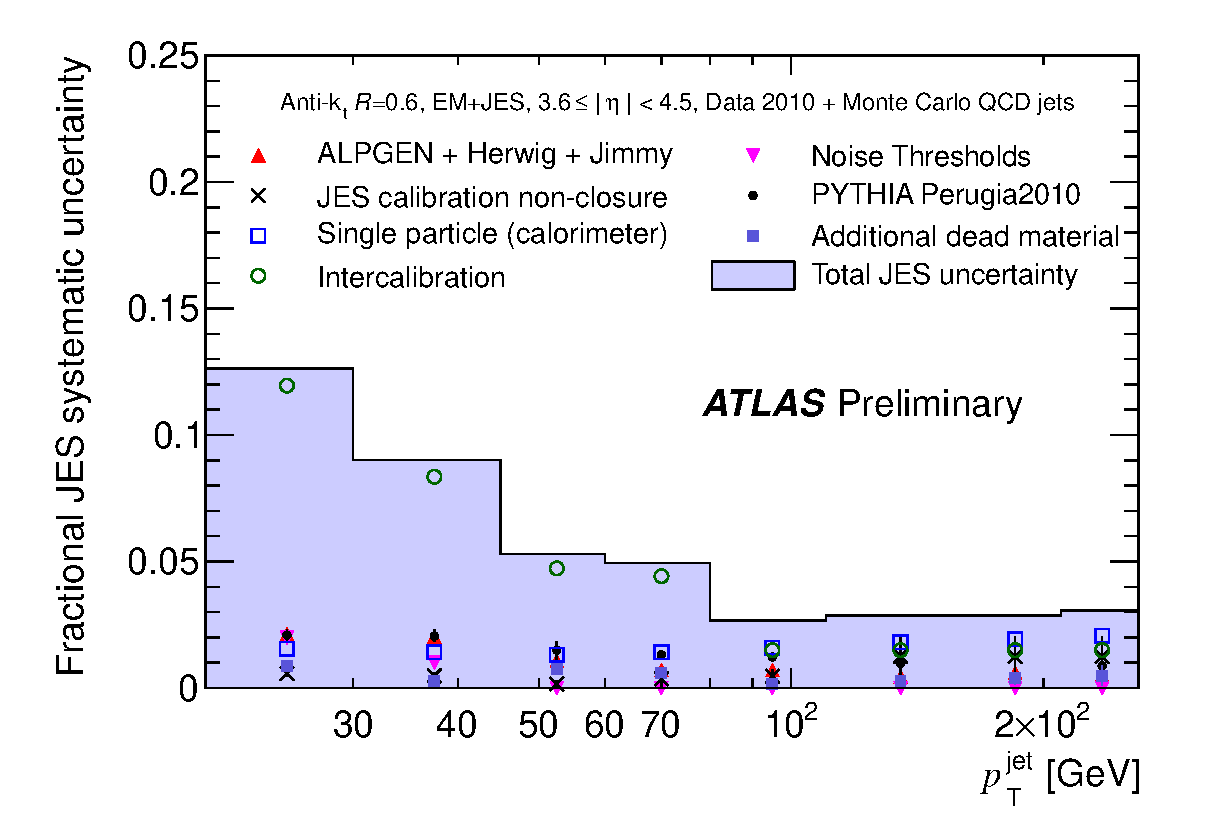
\includegraphics[width=0.45\linewidth,angle=0]{JES_fig_11}
%\label{JES_uncertainty_3_fig}
%}
%\end{centering}
%\label{JES_uncertainty_figs}
%\end{figure}
% \red{ update these plots, see int note}
%\begin{figure}[tbp]
%\centering
%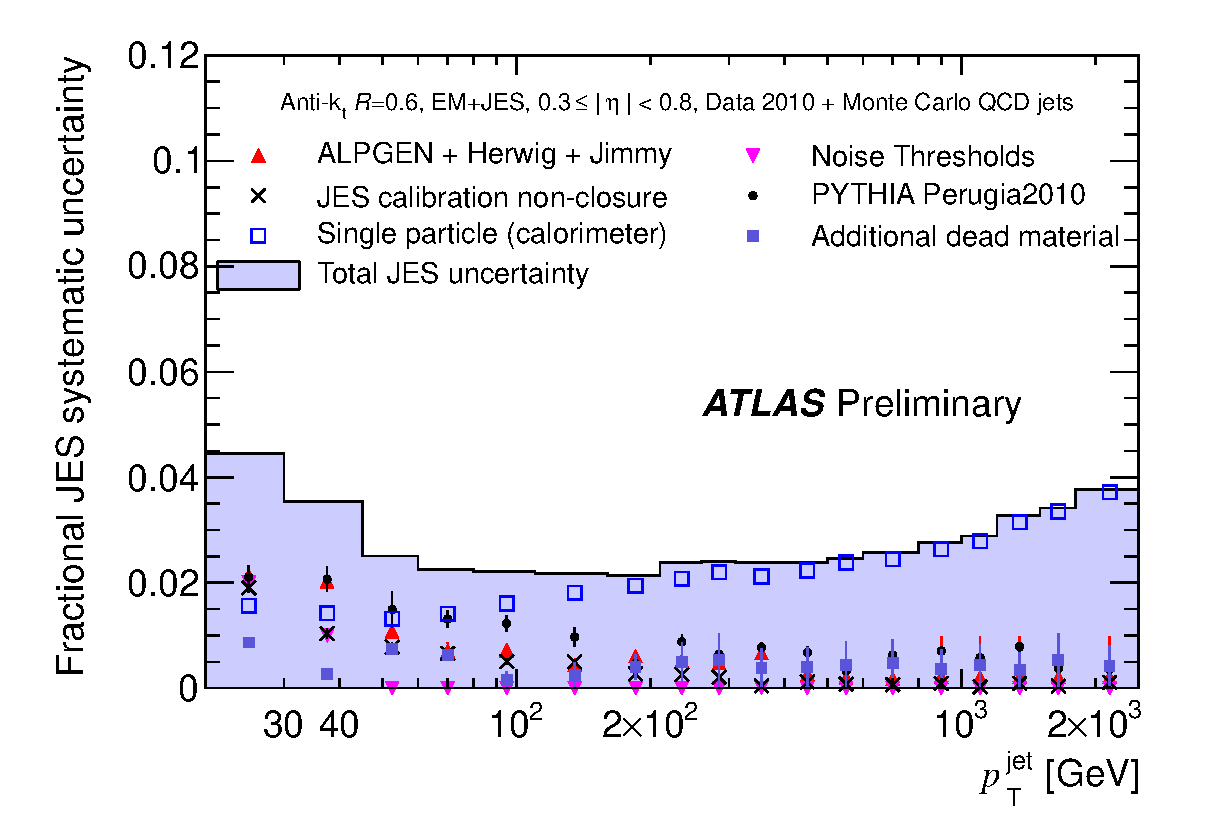
\includegraphics[width=0.85\linewidth,angle=0]{JESUncertainty_AntiKt6Topo_EMJES03-08.eps} 
%
%\caption{JES uncertainty in the central barrel region ($0.3 < |\eta | < 0.8$)}
%\label{JES_uncertainty_1_fig}
%\end{figure}
%
%\begin{figure}[tbp]
%\centering
%%\subfigure[caption 1]{
%%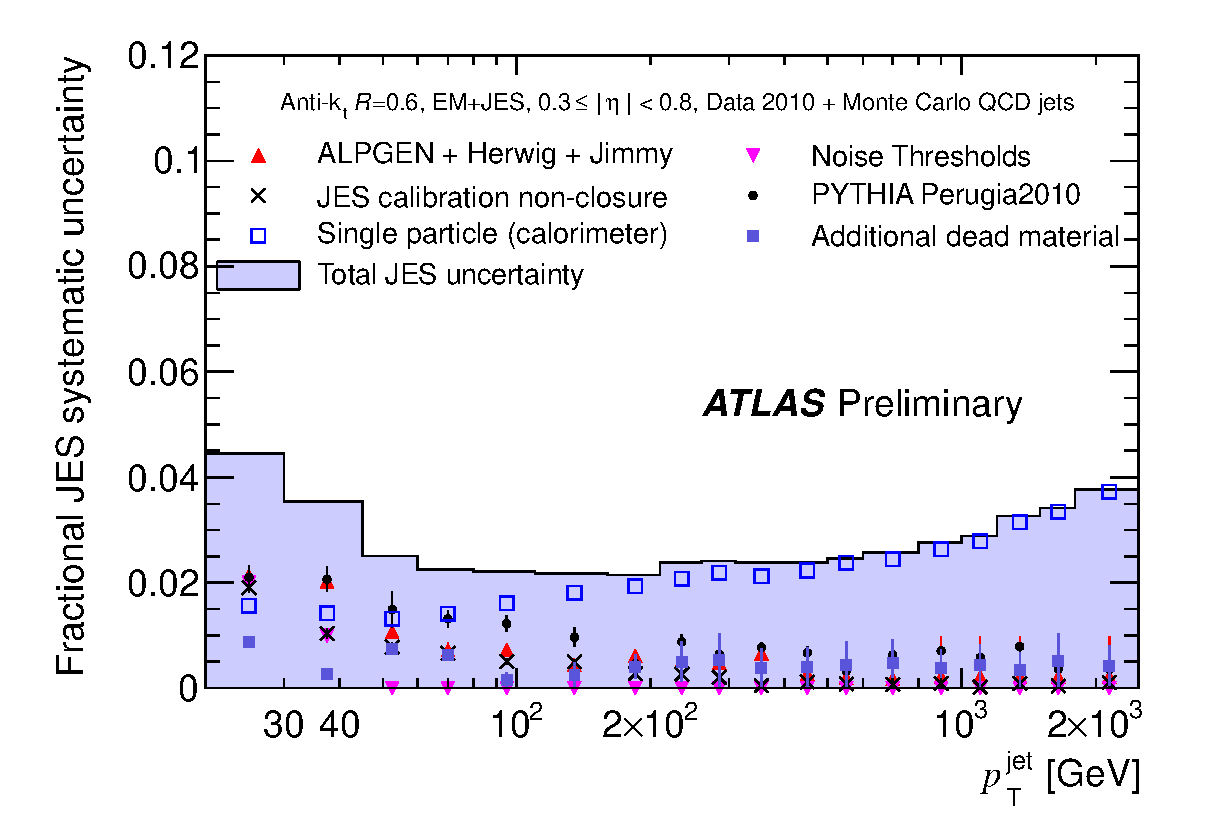
\includegraphics[width=0.85\linewidth,angle=0]{JES_fig_09}
%%\label{JES_uncertainty_1_fig}
%%}\\
%\subfigure{
%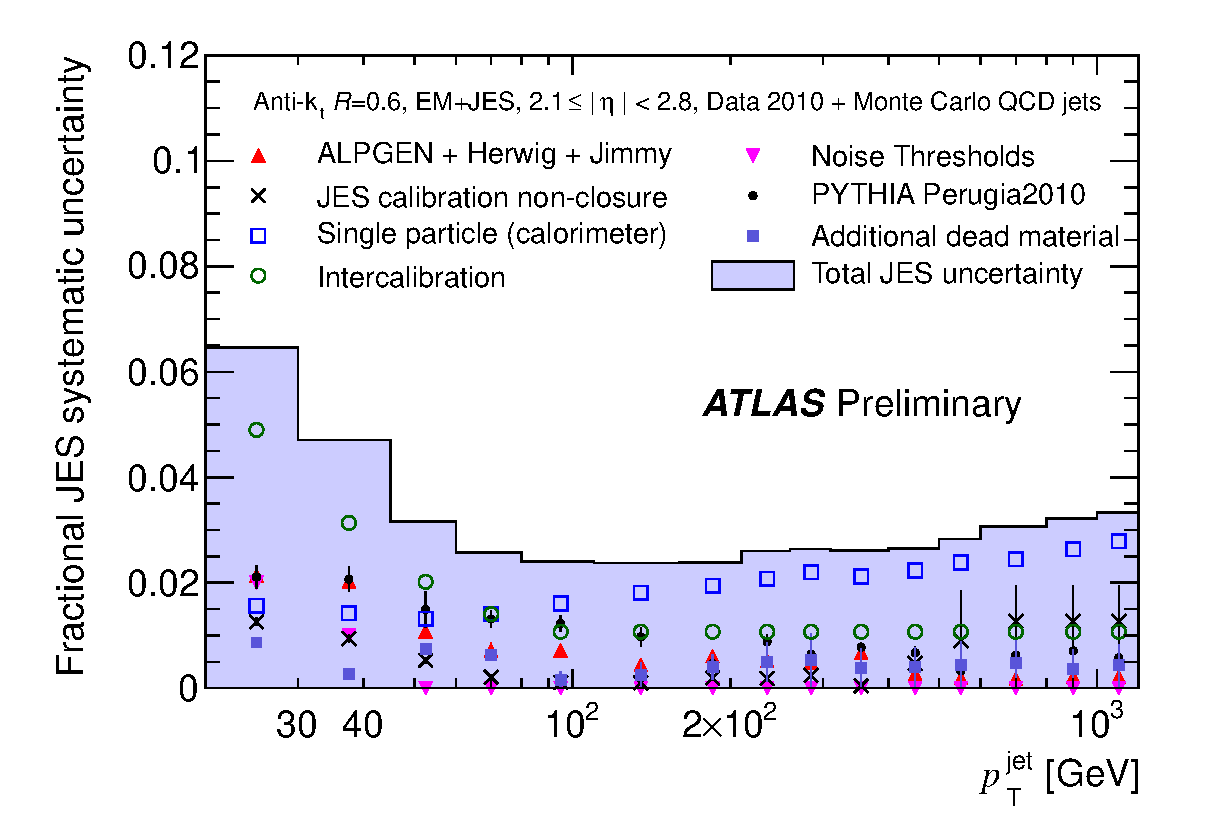
\includegraphics[width=0.85\linewidth,angle=0]{JESUncertainty_AntiKt6Topo_EMJES21-28.eps}
%\label{JES_uncertainty_2_fig}
%}\\
%
%\subfigure{
%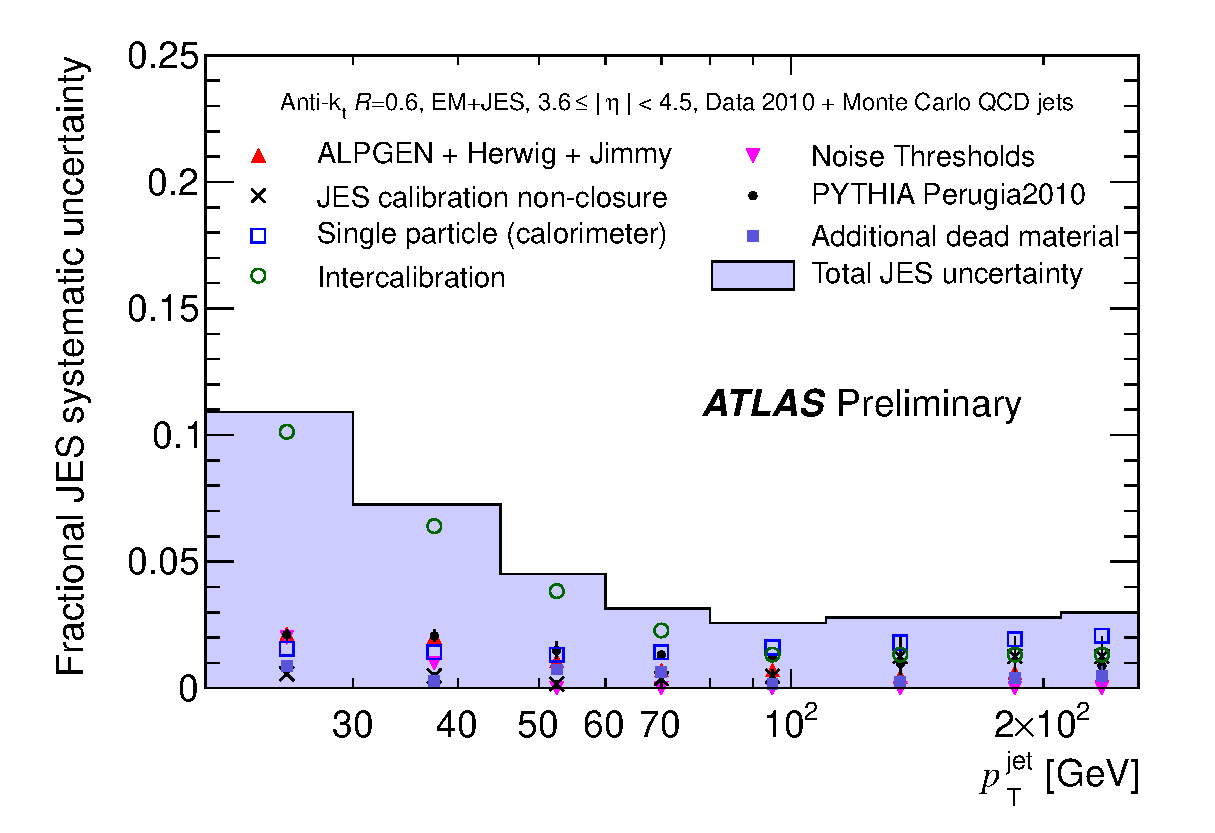
\includegraphics[width=0.85\linewidth,angle=0]{JESUncertainty_AntiKt6Topo_EMJES36-45.eps}
%\label{JES_uncertainty_3_fig}
%}
%\caption{ JES uncertainty for  the end-cap  ($2.1 < |\eta | < 2.8$)  and FCal ($3.1 < |\eta | < 4.5$). At low \pt, the intercalibration provides the dominant source of uncertainty.} 
%\label{JES_uncertainty_figs}
%\end{figure}

%\begin{figure}[tbp]
%\begin{center}
%\subfigure[]{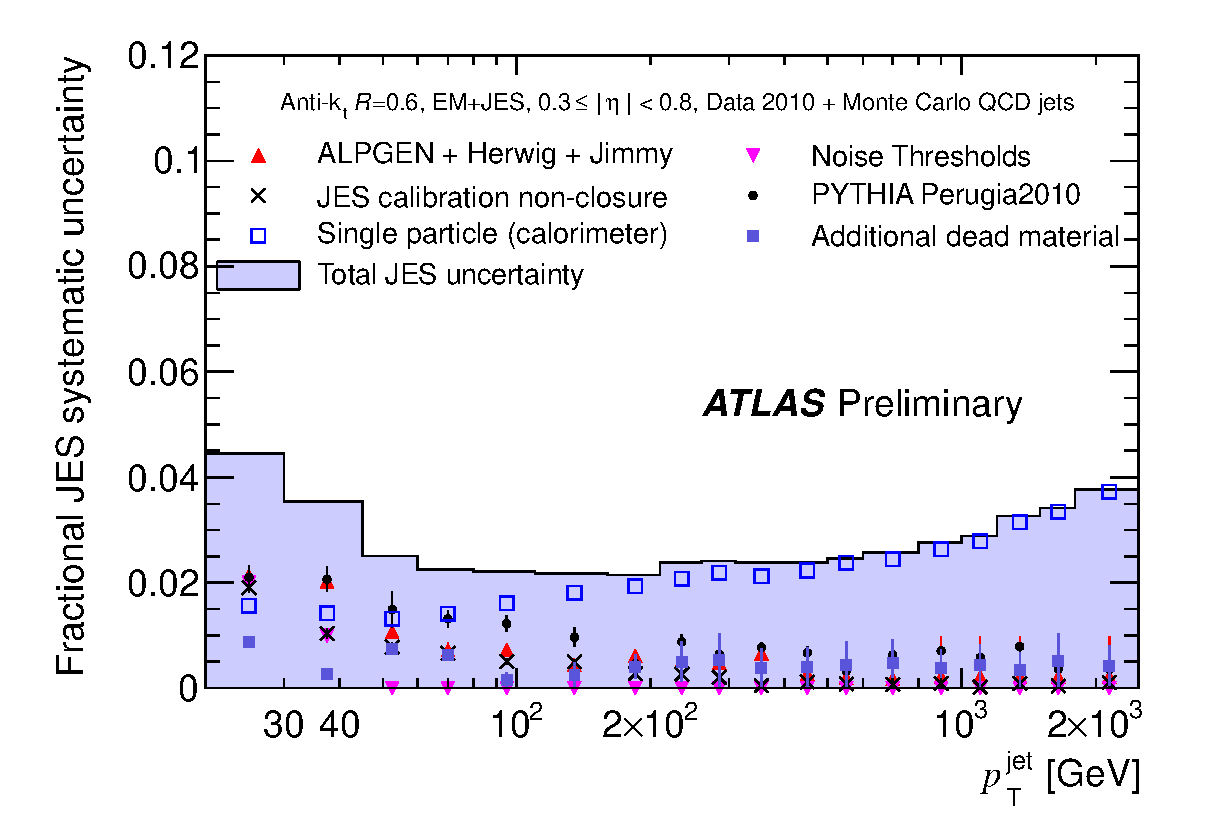
\includegraphics[width=0.6\linewidth,angle=0]{inclusive_results/figs_new/JES_3_8.eps}
%\label{JES_uncertainty_1_fig}} \\
%\subfigure[]{
%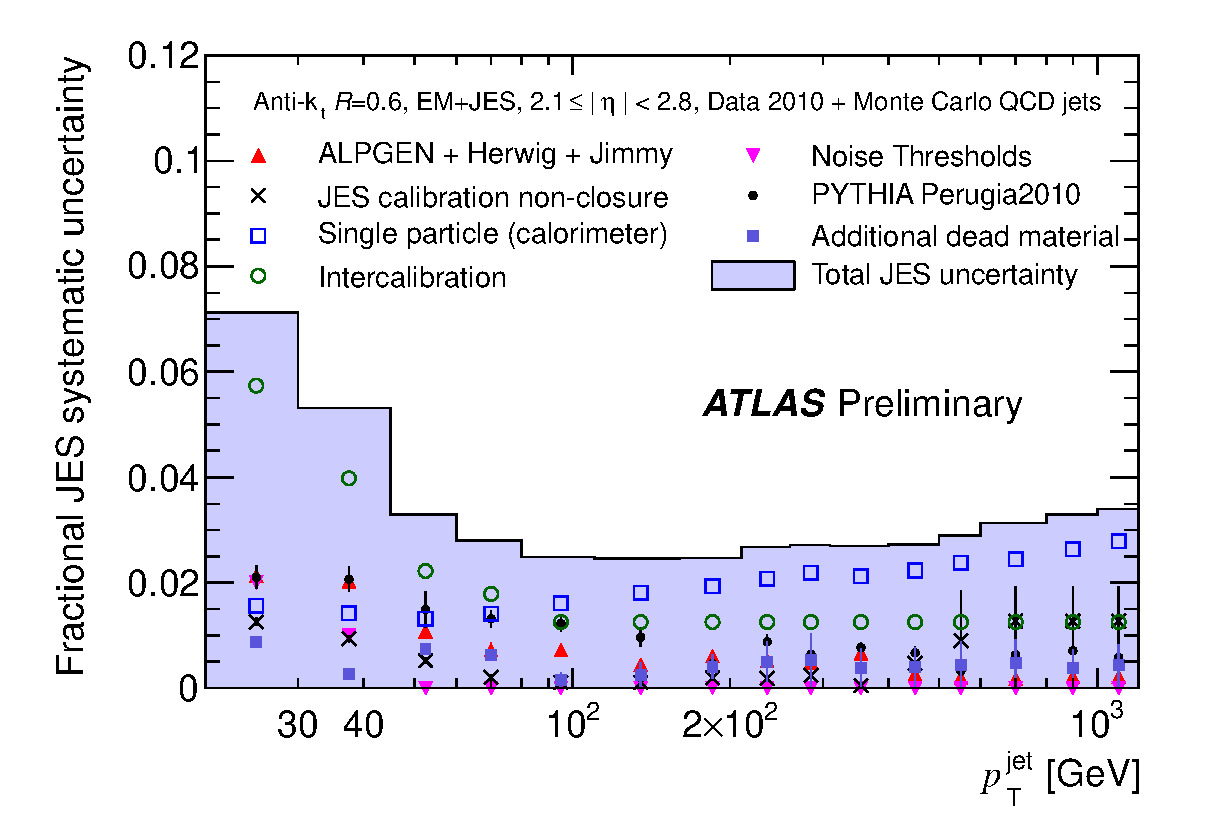
\includegraphics[width=0.6\linewidth,angle=0]{inclusive_results/figs_new/JES_21_28.eps}
%\label{JES_uncertainty_2_fig}
%}\\
%\subfigure[]{
%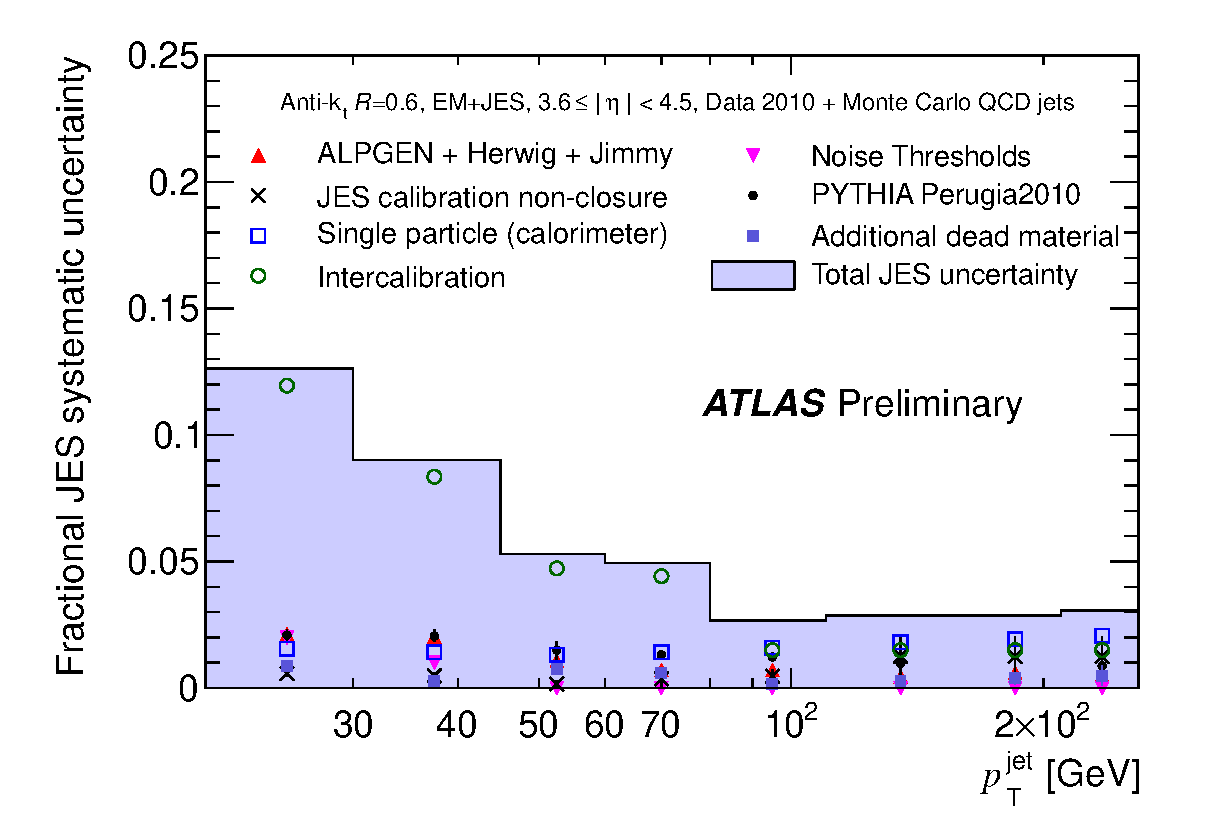
\includegraphics[width=0.6\linewidth,angle=0]{inclusive_results/figs_new/JES_36_45.eps}
%\label{JES_uncertainty_3_fig}
%}
%\end{center}
%\caption[Jet Energy Scale systematic uncertainty]{Systematic uncertainty on the Jet Energy Scale for jets in the regions (a) $0.3 < |\eta| < 0.8$, (b) $2.1 < |\eta| < 2.8$, (c) and $3.6 < |\eta| < 4.5$ \cite{ATLAS_JES_2010} }
%\label{JES_uncertainty_figs}
%\end{figure}
\begin{figure}[tbp]
\begin{center}
\subfigure[]{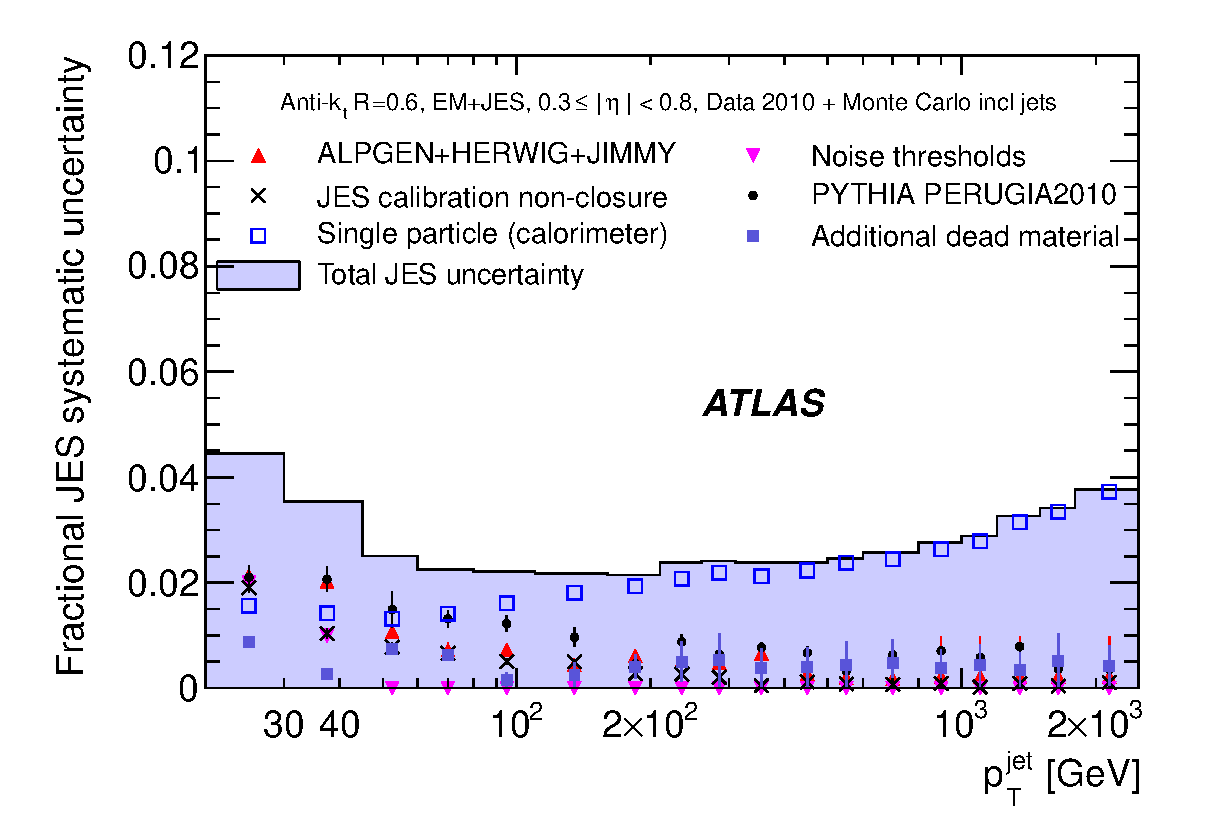
\includegraphics[width=0.6\linewidth,angle=0]{JES_new/fig_22a.eps}
\label{JES_uncertainty_1_fig}} \\
\subfigure[]{
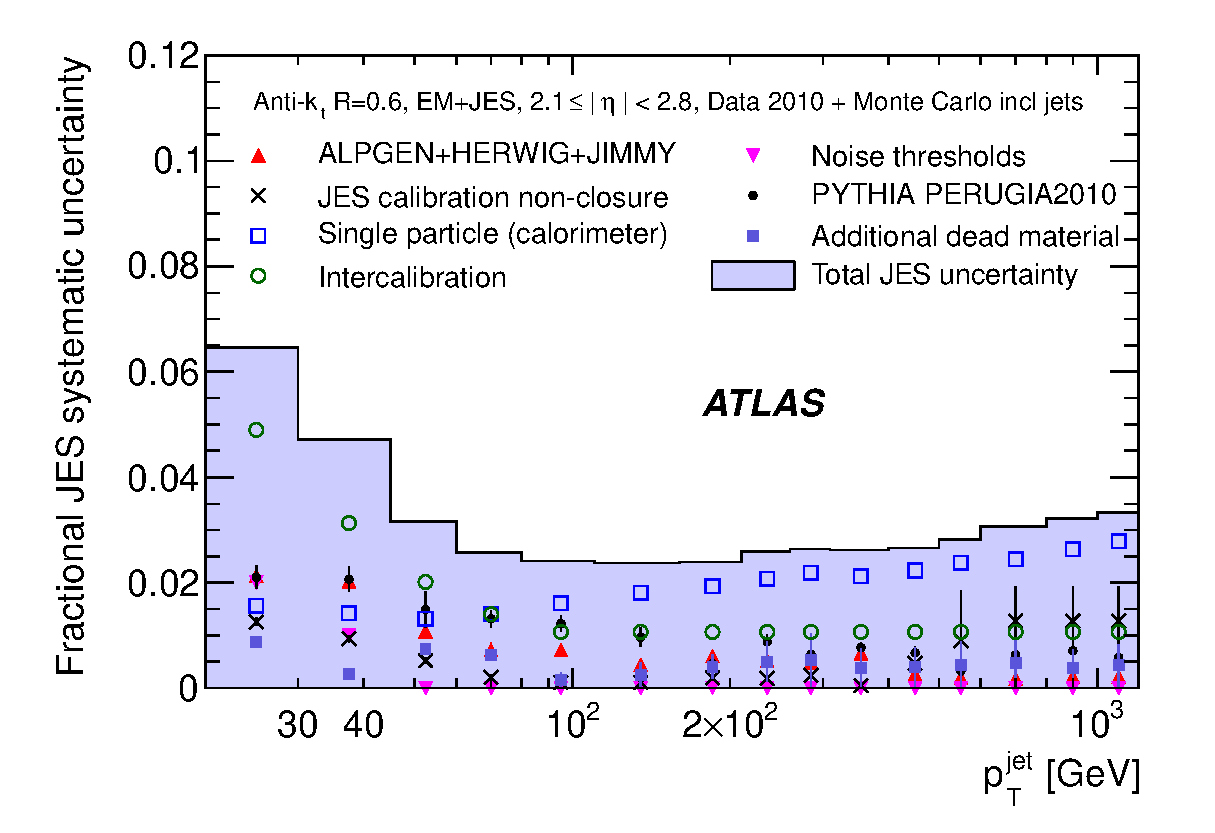
\includegraphics[width=0.6\linewidth,angle=0]{JES_new/fig_22b.eps}
\label{JES_uncertainty_2_fig}
}\\
\subfigure[]{
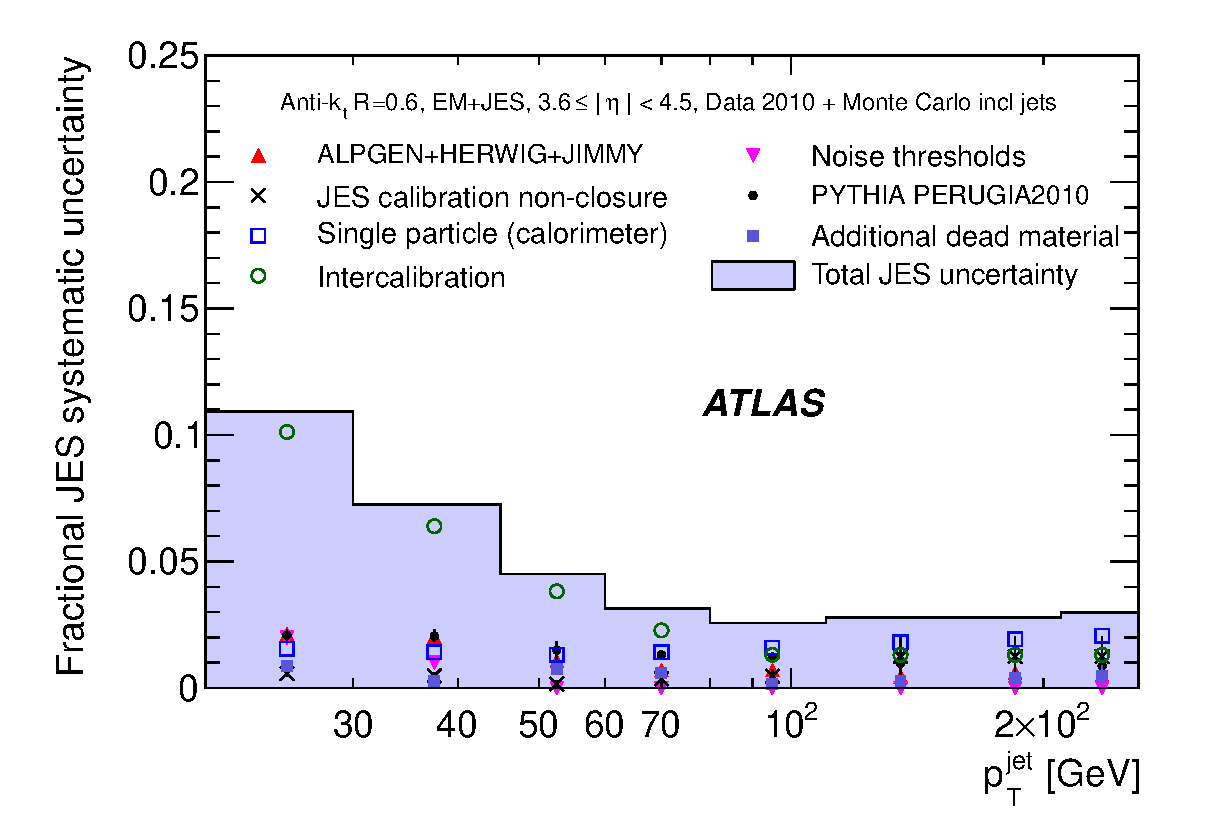
\includegraphics[width=0.6\linewidth,angle=0]{JES_new/fig_22c.eps}
\label{JES_uncertainty_3_fig}
}
\end{center}
\caption[Jet Energy Scale systematic uncertainty]{Systematic uncertainty on the Jet Energy Scale for jets in the regions (a) $0.3 < |\eta| < 0.8$, (b) $2.1 < |\eta| < 2.8$, (c) and $3.6 < |\eta| < 4.5$ \cite{JES_pub} }
\label{JES_uncertainty_figs}
\end{figure}


%\caption{JES uncertainty in the central barrel region ($0.3 < |\eta | < 0.8$)}
%\label{JES_uncertainty_1_fig}
%\end{figure}
%
%\begin{figure}[tbp]
%\centering
%%\subfigure[caption 1]{
%%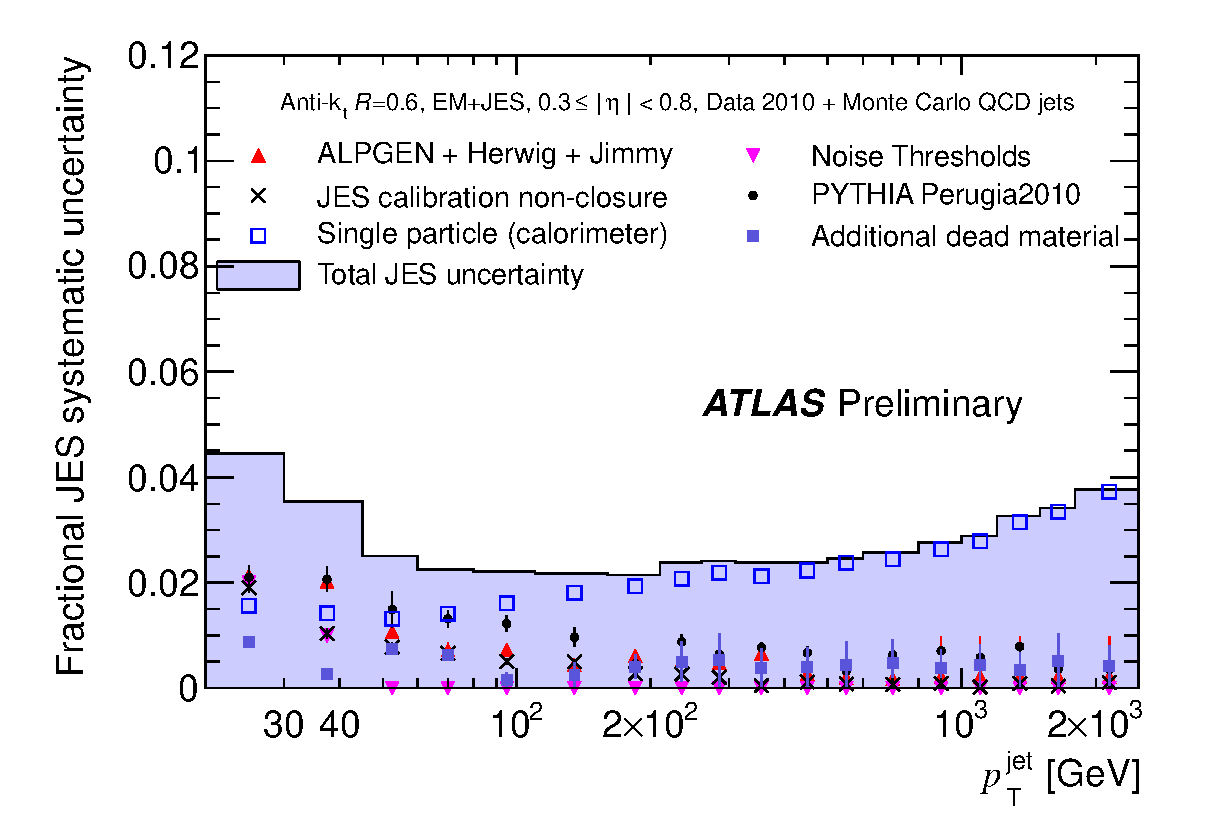
\includegraphics[width=0.85\linewidth,angle=0]{JES_fig_09}
%%\label{JES_uncertainty_1_fig}
%%}\\
%\subfigure{
%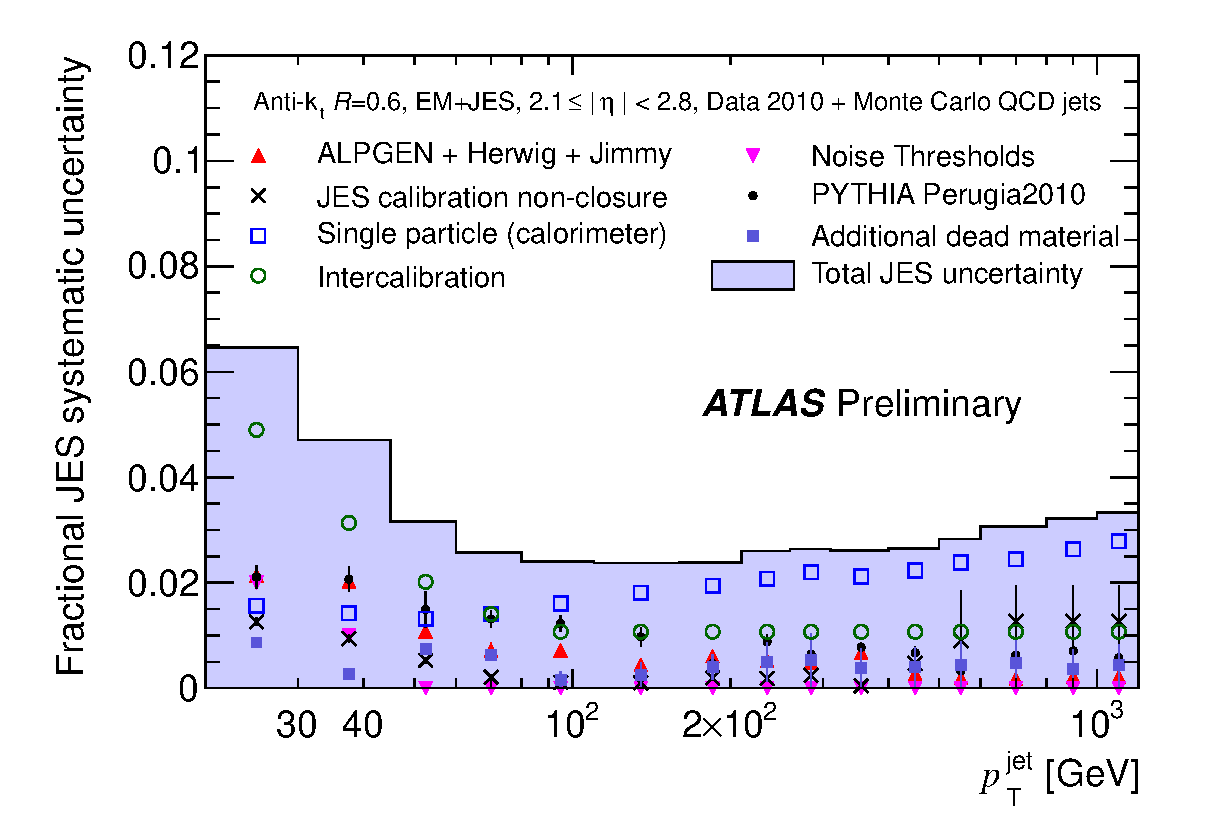
\includegraphics[width=0.85\linewidth,angle=0]{JESUncertainty_AntiKt6Topo_EMJES21-28.eps}
%\label{JES_uncertainty_2_fig}
%}\\
%
%\subfigure{
%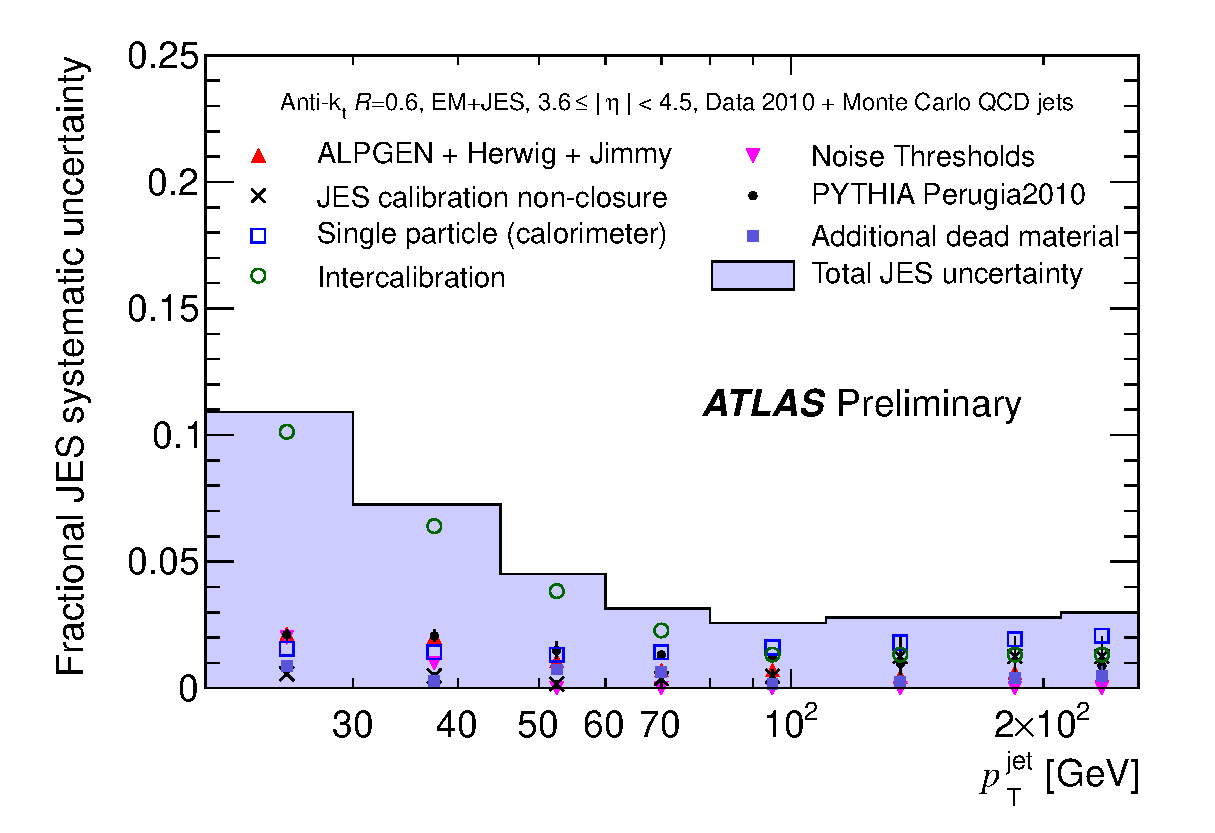
\includegraphics[width=0.85\linewidth,angle=0]{JESUncertainty_AntiKt6Topo_EMJES36-45.eps}
%\label{JES_uncertainty_3_fig}
%}
%\caption{ JES uncertainty for  the end-cap  ($2.1 < |\eta | < 2.8$)  and FCal ($3.1 < |\eta | < 4.5$). At low \pt, the intercalibration provides the dominant source of uncertainty.} 
%\label{JES_uncertainty_figs}
%\end{figure}




\cmt{


There are a number of contributions to the systematic uncertainty on the JES. 

comparison of in situ and single pion testbeam measurements

dead material budget (and uncertainty)

noise?

Monte Carlo


effects of these things are estimated using MC, by varying the item in question and observing how things vary.


1. uncertainty from the calibration method
2. uncertainty in calorimeter response
3. uncertainty in detector simulation (dead material)
4. uncertainty due to event generator/physics model
5. uncertainty in relative calibration

1. looking at nominal sample in eta, \pt, response (calibrated/truth) shows small deviations from unity (non-closure). 
method assumes that every constituent requires same average correction.
same correction factor for energy and \pt~is used. In cases where the calibrated jet mass is not equal to the truth jet mass, this correction results in a bias in \pt~calibration.

uncertainty taken as largest deviation of response (in \pt~and energy) from unity,
 is ~ 2\% for jets at low \pt~in barrel, less than 1\% for jets with \pt~> 30GeV elsewhere 

non-closure and non-unity of the response are treated as different things???

uncertainty in calorimeter response. E/P measurement propagated to JES. 1.5-4\%, depending on jet \pt.

Detector simulation:
*noise
1\% (2\%) for \akt jets with R=0.4 (R=0.6) for 20 GeV < \ptJet < 30 GeV
1\% for 30 GeV <ptjet<  45 GeV
negligible above 45 GeV

*dead material
vary amount of dead material, measure effect on jet response.
uncertainties due to relative calibration between barrel and end-cap/forward region


inter calibration for forward jets??
}

\subsection{Jet Selection}

%After jets have been calibrated, there are some criteria that they need to meet before being included in the analysis. Certain detector issues are capable of causing a jet to be reconstructed even if there were no physical particles depositing energy in that region of the calorimeter. Alternatively, other particles such as electrons or cosmic muons may be mistakenly reconstructed as jets. Jet ``cleaning'' cuts were made to address these issues, and remove from the analysis as many ``fake'' jets as possible. The jet cleaning cuts, and the problems they are intended to address, are listed below

%After jets have been calibrated, they are required to pass ``cleaning cuts'' before being included in the analysis. These criteria are intended to reject ``fake'' jets that do not originate from physical energy deposits resulting from proton-proton collisions.

After jets have been calibrated, they are required to pass ``cleaning cuts'' before being included in the cross-section analysis. The cleaning cuts are intended to reject ``fake'' jets, which can be reconstructed from calorimeter signals that do not originate from proton proton collisions.  The most significant sources of these fake jets are coherent noise in the EMB, noise bursts in the HEC, cosmic rays, and beam background events. The cleaning cuts used to reject fake jets are summarised below:




%There were several detector issues that occurred during data taking which could cause the and adversely effected the The cleaning cuts are summarised below.


%	// EM coherent noise
%	//medium
%	if ((myemf>0.90) &&(fabs(myLArQuality) >0.8) && (fabs(EMscale_JetEta) <2.8)) clean = false;
%	
%	// HEC spike
%	//loose
%	if ((myhecf > 0.5 )&& (fabs(myHECQuality)>0.5) ) clean = false;
%	if (fabs(myNegativeE) >60000.0) clean = false;
%	//medium
%	if ((1 - fabs(myHECQuality) )< myhecf) clean = false;
%	
%	
%	//cosmics / beam background
%	if (fabs(myTiming)>10) clean = false;
%	if ((myemf < 0.05 )&& (mychf < 0.1)&& (fabs(EMscale_JetEta) < 2.0)) clean = false; // medium
%	if ((myemf < 0.05 )&& (fabs(EMscale_JetEta) > 2.0)) clean = false;
%	if (myfMax > 0.99 && fabs(EMscale_JetEta) < 2.0) clean = false;
%	// medium
%	if ((myemf > 0.95 )&& (mychf < 0.05)&& (fabs(EMscale_JetEta) < 2.0)) clean = false;

\begin{itemize}
\item{\bf Coherent noise in the EM calorimeter:} Jet candidates with $|\eta| < 2.8$ were rejected if \cmt{$EM_\mathrm{f}$} $f_\mathrm{em}$, the fraction of the jet energy deposited in the EM calorimeter, exceeded 0.9 while the LAr quality variable exceeded 0.8. The LAr quality is defined as the fraction of jet cells located in the EM calorimeter that have a pulse shape significantly different to that expected.
\item{\bf Noise bursts (``spikes'') in the HEC:} Jet candidates were rejected if the fraction of the jet energy deposited in the HEC was greater than $1 - HECQ$, where $HECQ$ is the HEC quality variable, defined as the fraction of the jets cells located in the HEC that have a pulse shape significantly different to that expected. Jets were also rejected if the sum of negative energy cells exceeded 60 GeV in magnitude.
\item{\bf Cosmics rays/beam background:} Jet candidates were rejected if the average timing for jet cells was greater than 10ns from the average event time, or if 99\% of the jet energy was deposited in a single layer of the calorimeter. For jets with $|\eta| < 2.0$, tracking information can be used to define the charged fraction, \cmt{$Chf$}$f_\mathrm{ch}$, which is the fraction of the jet \pt~associated with tracks in the inner detector. In this case, jets were rejected if $f_\mathrm{ch} < 0.1$ and $f_\mathrm{em} < 0.05$ or if $f_\mathrm{em} > 0.95$ and $f_\mathrm{ch} < 0.05$. Jets with $|\eta| > 2.0$ were rejected if $f_\mathrm{em} < 0.05$.
\end{itemize}

Jet candidates which failed these cleaning cuts were excluded from the analysis. The efficiency of these cleaning cuts for real jets was at least 96\% for jets with \pt~$> 20$~GeV, and greater than 99\% for jets with \pt~$>$~60~GeV. In kinematic regions where the jet cleaning efficiency was less than 99\%, the inefficiency is corrected for in the inclusive jet and dijet cross-section measurements.

%\clearpage
\section{Event Selection and Data Quality}
\label{sec::eventselection}
%%used full 2010 dataset, $45pb^{-1}$ before DQ, 37 after. Dq cuts require stable beams, all systems go, flag bad lumi blocks from noise bursts(\red{in HEC?}). SM GRL
%\red{DATA QUALITY DATA QUALITY DATA QUALITY}
%https://twiki.cern.ch/twiki/bin/viewauth/AtlasProtected/SMJetAnalysis2010#Good_Runs_List
%%lhc stablebeams T
%%725 ptag data10_7TeV
%%726 dq ATLGL LBSUMM#DetStatus-v03-repro05-01 g
%%727 dq L1CTP LBSUMM#DetStatus-v03-repro05-01 g
%%728 dq L1CAL LBSUMM#DetStatus-v03-repro05-01 g
%%729 dq atltor LBSUMM#DetStatus-v03-repro05-01 g
%%730 dq atlsol LBSUMM#DetStatus-v03-repro05-01 g
%%731 dq pix LBSUMM#DetStatus-v03-repro05-01 g
%%732 dq sct LBSUMM#DetStatus-v03-repro05-01 g
%%733 dq trtb,trte LBSUMM#DetStatus-v03-repro05-01 g
%%734 dq CP_TRACKING LBSUMM#DetStatus-v03-repro05-01 g
%%735 dq CP_MET_METCALO LBSUMM#DetStatus-v03-repro05-01 g
%%736 dq CP_JET_JETEC LBSUMM#DetStatus-v03-repro05-01 g
%%737 dq CP_JET_JETEA LBSUMM#DetStatus-v03-repro05-01 g
%%738 dq CP_JET_JETB LBSUMM#DetStatus-v03-repro05-01 g
%%739 dq CP_JET_JETFC LBSUMM#DetStatus-v03-repro05-01 g
%%740 dq CP_JET_JETFA LBSUMM#DetStatus-v03-repro05-01 g
%%741 dq LUMI LBSUMM#DetStatus-v03-repro05-01 g
%
%find run 166466-166964 and
%partition ATLAS
% and db DATA
%  and 
%  lhc stablebeams T and 
%  ptag data10_7TeV
%dq ATLGL LBSUMM#DetStatus-v03-repro05-01 g // someone looked at DQ stuff
%dq L1CTP LBSUMM#DetStatus-v03-repro05-01 g // no clock/data header problems
%dq L1CAL LBSUMM#DetStatus-v03-repro05-01 g  // trigger good
%dq atltor LBSUMM#DetStatus-v03-repro05-01 g //toroid
%dq atlsol LBSUMM#DetStatus-v03-repro05-01 g // solenoid
%dq pix LBSUMM#DetStatus-v03-repro05-01 g //pixel
%dq sct LBSUMM#DetStatus-v03-repro05-01 g // sct
%dq trtb,trte LBSUMM#DetStatus-v03-repro05-01 g /trt 
%dq CP_TRACKING LBSUMM#DetStatus-v03-repro05-01 g // tracking (vertex reconstruction?)
%dq CP_MET_METCALO LBSUMM#DetStatus-v03-repro05-01 g // missing ET from calo (not muons)
%dq CP_JET_JETEC LBSUMM#DetStatus-v03-repro05-01 g //
%dq CP_JET_JETEA LBSUMM#DetStatus-v03-repro05-01 g //
%dq CP_JET_JETB LBSUMM#DetStatus-v03-repro05-01 g //
%dq CP_JET_JETFC LBSUMM#DetStatus-v03-repro05-01 g //
%dq CP_JET_JETFA LBSUMM#DetStatus-v03-repro05-01 g // jet reconstruction good
%dq LUMI LBSUMM#DetStatus-v03-repro05-01 g // luminosity monitoring
%dq TRJET LBSUMM#DetStatus-v03-repro05-01 g // jet trigger slice good
%dq TRCAL LBSUMM#DetStatus-v03-repro05-01 g  // calo trigger
%dq IDBS LBSUMM#DetStatus-v03-repro05-01 y+   
%
%
%In order for an event to be considered in the inclusive jet cross-section analysis, it was required to meet certain data quality criteria. 
%These criteria are contained in a good run list (GRL), which specifies DQ requirements
%
% status of various atlas subsystems specified in terms of flags, GRL contains a list of flags that must be required. Given flag may be green, functioning normally, yellow flawed but perhaps recoverable, red bad. 
% For inclusive jet and dijet analysis, required
% 
% Trigger (L1 Calo and L1 CTP) operating normally
% Good operation of HLT also required for periods G-I
% magnets (toroid and solenoid) both operating normally
% inner detector (pixel, sct, TRT barrel, trt end cap) operating normally
% track reconstruction green
% missing ET reconstruction green - from Calo
% jet reconstruction green in barrel, end-cap, and FCal regions. end cap (EMEC & HEC calorimeters), FCal, EM barrel, TILE, (all calorimeters)
% LUMI??

%status of various atlas subsystems specified in terms of flags, GRL contains a list of flags that must be required. Given flag may be green, functioning normally, yellow flawed but perhaps recoverable, red bad. 
% For inclusive jet and dijet analysis, required

%In order to ensure that the detector was operating normally 
In order for an event to be considered in the inclusive jet and dijet cross-section measurements, it was required to meet certain Data Quality (DQ) criteria. These criteria were expressed in terms of DQ flags. A green flag indicated that the corresponding system was operating normally, whereas a yellow flag indicated an issue that could be corrected for offline, or data that could be used with caution. Red flags were used to indicate data that had some problems and should not be used.

In order for an event to be included in the inclusive jet and dijet cross-section measurements, the following DQ flags were required:
\begin{itemize}
\item Trigger (L1Calo and L1 CTP) were required to be green. For periods G-I, the HLT flag was also required to be green.
\item Magnets (toroid and solenoid) were required to be green.
\item Inner Detector subsystems (pixel, SCT and TRT) were required to be green.
\item Track, Missing $E_\mathrm{T}$ (from calorimeters), and Jet reconstruction performance were required to be green.
\item Luminosity monitoring was required to be green.
\end{itemize}



% Certain problems, such as noise bursts or high voltage issues, could occur from time to time. The data quality criteria were established to ensure that the detector was operating normally when the event was recorded, and to exclude events in which there was a known problem with the detector. \red{MORE ABOUT THIS}

 The event was also required to have a primary vertex with at least 5 tracks. Events were also required to pass a trigger condition, which is discussed below.
% Each \pt-$y$ bin in the analysis was associated with a particular trigger. The trigger condition for a given bin was required to be satisfied before an event could contribute jets to that bin.

These criteria were required for both the inclusive jet  and dijet cross-section measurements. Both of these analyses considered jets in the rapidity range $|y| < 4.4$. The inclusive jet cross-section measurement considered jets with $\pt > 20$ GeV, while the measurement of the dijet mass spectrum required that the leading jet in the event have $\pt > 30$ GeV and the subleading jet have $\pt > 20$ GeV.


\subsection{Triggers used for the inclusive jet analysis}
%The measurement is divided into 7 bins of rapidity. The 
\label{incjet_triggers}

The inclusive jet cross-section measurement is performed in 7 bins of rapidity and 16 bins of \pt. A dedicated, fully efficient trigger is used to collect jets in each bin in order to maximise statistics. Each bin has an associated  trigger condition that the event needed to satisfy before jets from the event could contribute to that bin. The three lowest \pt~bins are populated using data taken from the MBTS1 (minimum bias) trigger, which required a hit signal from at least one of the MBTS tiles (described in Section~\ref{sec_triggers}). Minimum bias data from only the three earliest periods of running (A-C) were used for this purpose, as in these periods this trigger had a lower prescale (and so more data was recorded) and there was a minimal amount of pile-up. At higher \pt~(above 60 GeV), data was taken using the central jet trigger for jets with $|y| < 2.8$. The rapidity bin from $2.8 < |y| < 3.6$ is referred to as the ``transition bin'', as it covers the transition region between the end-cap calorimeters and the FCal (Figure~\ref{end_cap_xsec_2}). In this region both the central and forward jet triggers were used, whereas in the forward region ($3.6 < |y| < 4.4$) only the forward jet trigger was used. 

%\begin{figure}
%\centering 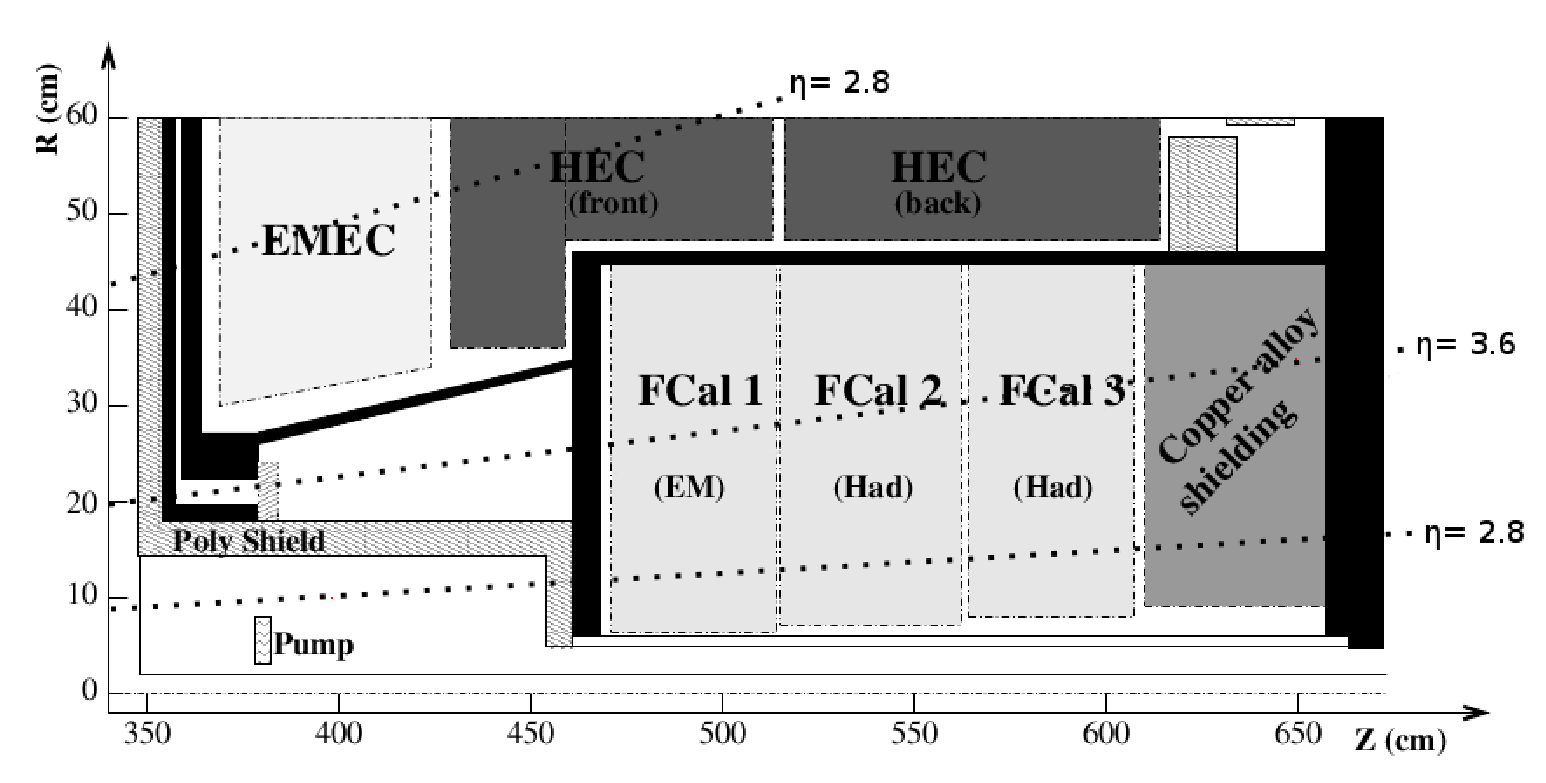
\includegraphics[width=0.8\linewidth]{atlas_EC_xsec}
%\caption{diagram showing cross-section of part of an end-cap in ATLAS. The forward bin corresponds approximately to the region $2.8 < |\eta| < 3.6$, and is completely contained within the FCal. The transition bin covers the area between $|\eta| = 2.8$ and $|\eta| = 3.6$, which is partially occupied by both the end-cap calorimeters and the FCal.}
%\label{transition_xsec}
%\end{figure}





%\red{MORE DETAIL HERE. this is the stuff I did, so I can talk more about it. per jet efficiency, inclusive efficiency / jet by jet versus event level efficiency. binning in pt, reference, triggers studied. L1, L2 chains.}

The performance of the jet trigger system needs to be understood before it can be used effectively in the analysis. This \cmt{understanding} is achieved by measuring the trigger efficiency. The per-jet efficiency of a trigger represents the probability that the trigger condition will be satisfied by a given jet. It is defined as 
\begin{equation}
\epsilon_\mathrm{per-jet} = \frac{N_\mathrm{triggered}}{N_\mathrm{reference}} ,
\end{equation}
where $N_\mathrm{reference}$ is the number of reconstructed jets obtained from a reference sample and $N_\mathrm{triggered}$ is the number of reconstructed jets from this reference sample that satisfy the trigger condition. These quantities are binned in terms of the \pt~and rapidity of the reconstructed jets, which allows the efficiency to be determined as a function of these variables. For the trigger studies presented here, data taken from the MBTS1 trigger was used to obtain the reference sample.

In order to count $N_\mathrm{triggered}$, the reconstructed jets that satisfy the trigger condition need to be identified. L1 jet triggers are satisfied provided that the transverse energy deposited in a given ROI exceeds a certain threshold (as discussed in Section~\ref{sec_triggers}). In order to determine whether a given jet satisfies the trigger condition, it must be matched to an ROI that is above the trigger threshold. A reconstructed jet is matched to an ROI from the central jet trigger if the jet lies within $\Delta R \leq 0.4$ of the ROI in $\eta-\phi$ space. The forward jet trigger relies only on data from the FCal, and the trigger towers in the FCal are summed such that there is no granularity in $\eta$. Reconstructed jets are matched to a forward jet trigger ROI if the jet lies within $\Delta \phi \leq 0.4$ of the ROI, provided the two are on the same side of the detector.

The per-jet efficiency describes the probability that the trigger will be satisfied by a given jet.
However, for events containing multiple jets, only one jet needs to satisfy the trigger condition in order for all of the jets\footnote{ That is, all of the jets that have passed the jet selection criteria described earlier.} to count towards the inclusive cross-section measurement. Consider an event in which there are two jets with equal and opposite momenta. If the relevant trigger has a per-jet efficiency of 90\%, then each jet has a 10\% chance of not satisfying the trigger condition. There is thus only a 1\% chance that neither jet satisfies the trigger condition, and thus a 99\% probability that the trigger condition is satisfied by one or both jets. For this reason, it is more appropriate to use the inclusive efficiency, $\epsilon_\mathrm{inc}$, which is defined as
\begin{equation}
\epsilon_\mathrm{inc} = \frac{N_\mathrm{triggered,inc}}{N_\mathrm{reference}}.
\end{equation}
In this case, $N_\mathrm{triggered,inc}$ is the number of jets contained in events (taken from the reference sample) in which the trigger condition is satisfied. The inclusive efficiency describes the efficiency of the trigger at the event level: if any jet in the event satisfies the trigger condition, then all jets in the event are counted. The inclusive efficiency is thus used to determine the \pt~range in which data collected by a given trigger will be used. 


% note that no matching needs to be done for the inclusive efficiency





%reference sample unbiased
%
%trigger condition - et in ROI
%
%matching

%bin jet numbers in terms of pt and rapidity, measure efficiency as a function of these variables.





%The inclusive efficiency of a trigger is defined as 
%
%\begin{equation}
%\epsilon_\mathrm{inclusive} = \frac{N_\mathrm{triggered}}{N_\mathrm{reference}} ,
%\end{equation}
%
%where $N_{reference}$ is the total number of jets reconstructed offline from a reference sample, and $N_{triggered}$ is the number of reconstructed jets coming from events in the reference sample which pass the trigger condition. This efficiency is then binned in the \pt~of the reconstructed jets to produce a turn-on curve. Trigger efficiencies for the transition and forward bins are plotted in Figures~\ref{figures_trans} and~\ref{figures_forward}, respectively. 



In order to reduce the uncertainties on the cross-section related to the trigger efficiency, data are only used when collected above the trigger's ``plateau'' point. The plateau point is defined by integrating bins of $N_\mathrm{triggered,inc}$ and $N_\mathrm{reference}$ from high \pt~towards low \pt, until reaching the point where the ratio of these sums drops below 99\%. The high edge of this bin is then taken as the plateau point, as the trigger is at least 99\% efficient at \pt~values above it. On the plateau, the trigger is treated as fully efficient, and is used to collect data for the appropriate \pt~bins. 

While studying the forward jet triggers, it was observed that events containing high \pt~jets in the region $3.4 < \eta<3.9$ and $-\pi/8 < \phi < 0$ were not being selected by the trigger.\cmt{The L1 trigger tower in this region was producing very little signal, and was effectively dead} The L1 trigger tower in this region was found to be producing no signal. This reduced the geometrical acceptance of the forward jet trigger by $\frac{1}{128}$\footnote{The dead region consists of one of the four trigger towers in one of the sixteen $\phi$-slices of one of the two forward calorimeters.}, which is corrected for in the cross-section calculation. Consequently, the plateau points in the forward and transition bins are defined at an efficiency of 98\%. It should be noted that while the trigger tower is considered ``dead'', the calorimeter cells (and hence jet reconstruction) are unaffected in this region, as the cell information is read off the FEB separately from the trigger signal (as described in Section \ref{sec_FEB}).

%As data taking progressed, the trigger system was commissioned further. An error was found during early running which meant that the forward jet trigger was unreliable before period E5 ( run 161118). For the remainder of periods E and F the forward trigger was active at L1, and so data collected by it during these periods was used in the analysis. For periods G through I, the HLT was enabled, and so trigger decisions were also made at level 2. The trigger algorithms used for each bin during different data taking periods are shown in table XX.

The forward jet triggers were not commissioned when data taking began in 2010, however as the year progressed, the trigger system was commissioned further. The forward jet triggers were commissioned after run 161118 (during period E), and were used to collect data in the forward and transition regions from then on. The HLT system was commissioned from period G on, which allowed event rejection to occur at L2. The EF remained in ``pass-through'' mode throughout the remainder of 2010, meaning that all events selected at L2 were recorded. Triggers at L1 were used to collect data until the HLT was commissioned, after which L2 triggers were used (periods G-I). 

The inclusive efficiencies for the transition and forward bins are plotted in Figures~\ref{figures_forward} and~\ref{figures_trans}, respectively, for several trigger thresholds at L1 and at L2. At L1, the trigger thresholds are based on the EM scale transverse energy reconstructed at L1, L1 $E_\mathrm{T}^\mathrm{EM}$. For the forward bin (Figures~\ref{fig_forward4_eff} and \ref{fig_forward6_eff}) the efficiencies of the L1\_FJ10, L1\_FJ30, and L1\_FJ55 triggers are plotted, which require L1~$E_\mathrm{T}^\mathrm{EM}$ to be greater than 10 GeV, 30 GeV, and 55 GeV, respectively. The lowest threshold, L1\_FJ10, reaches its plateau point at 21 GeV for (calibrated) jets with $R$ = 0.4 and at 23 GeV for jets with $R$ = 0.6, and is thus used to collect data for the 30-45 GeV, 45-60 GeV, and 60-80 GeV \pt~bins in the forward rapidity bin. \cmt{L1 triggers were used in the forward regions for periods E (after run 161118) and F, after which the L2 triggers were commisioned and used to collect data (i.e. for periods G-I).} For periods G-I, trigger thresholds at L2 were used instead of L1. The lowest threshold forward jet trigger at L2, L2\_fj25, requires the L2 jet to have an EM scale transverse energy (L2 $E_\mathrm{T}^\mathrm{EM}$) of at least 25 GeV, while the higher thresholds, L2\_fj45 and L2\_fj70, require 45 GeV and 70 GeV, respectively. The L2\_fj25 threshold reaches its plateau point at 43 (45) GeV for jets with $R$ = 0.4 ($R$=  0.6), and is used to collect data for the 60-80 GeV and 80-110 GeV \pt~bins of the forward rapidity bin during periods G-I. Triggers for the transition bin use an ``OR'' method that will be discussed below, such that the event may be accepted by either the forward jet or the central jet trigger. For example, the lowest threshold used at L1 in the transition bin (Figures~\ref{fig_trans4_eff} and \ref{fig_trans6_eff}) requires that the event be selected by either the L1\_FJ10 or the L1\_J10 trigger, both of which require L1 $E_\mathrm{T}^\mathrm{EM} > 10$ GeV.

\begin{figure}[tbp]
\begin{centering}
\subfigure[]{
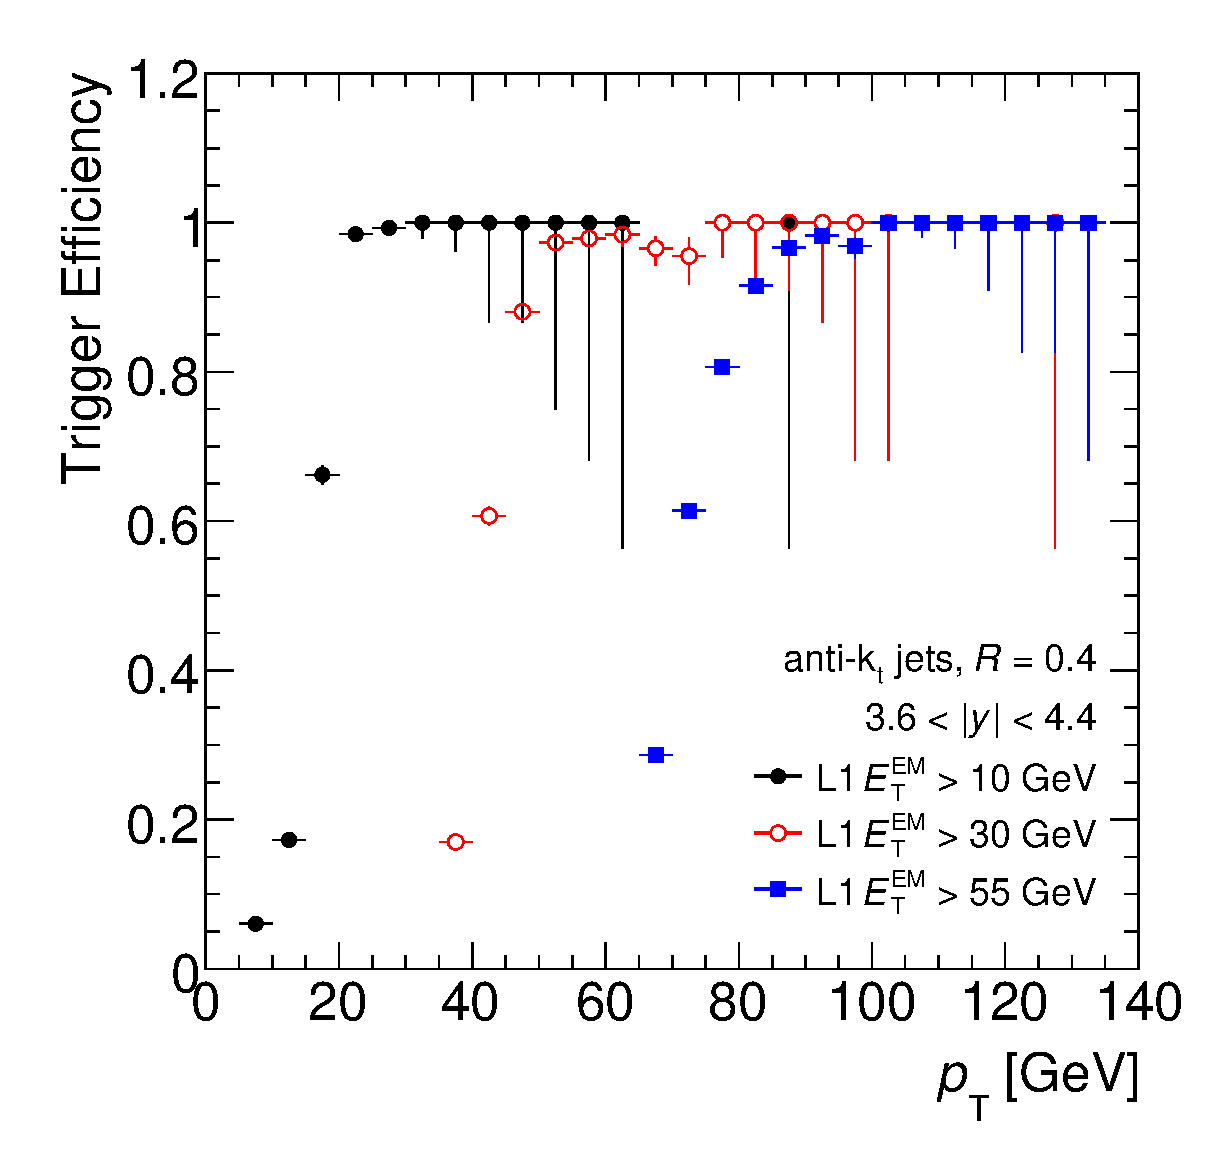
\includegraphics[width=0.45\linewidth,angle=0]{L1_triggers_forward_bin_akt4.eps}
\label{fig_forward4_eff}
}
\subfigure[]{
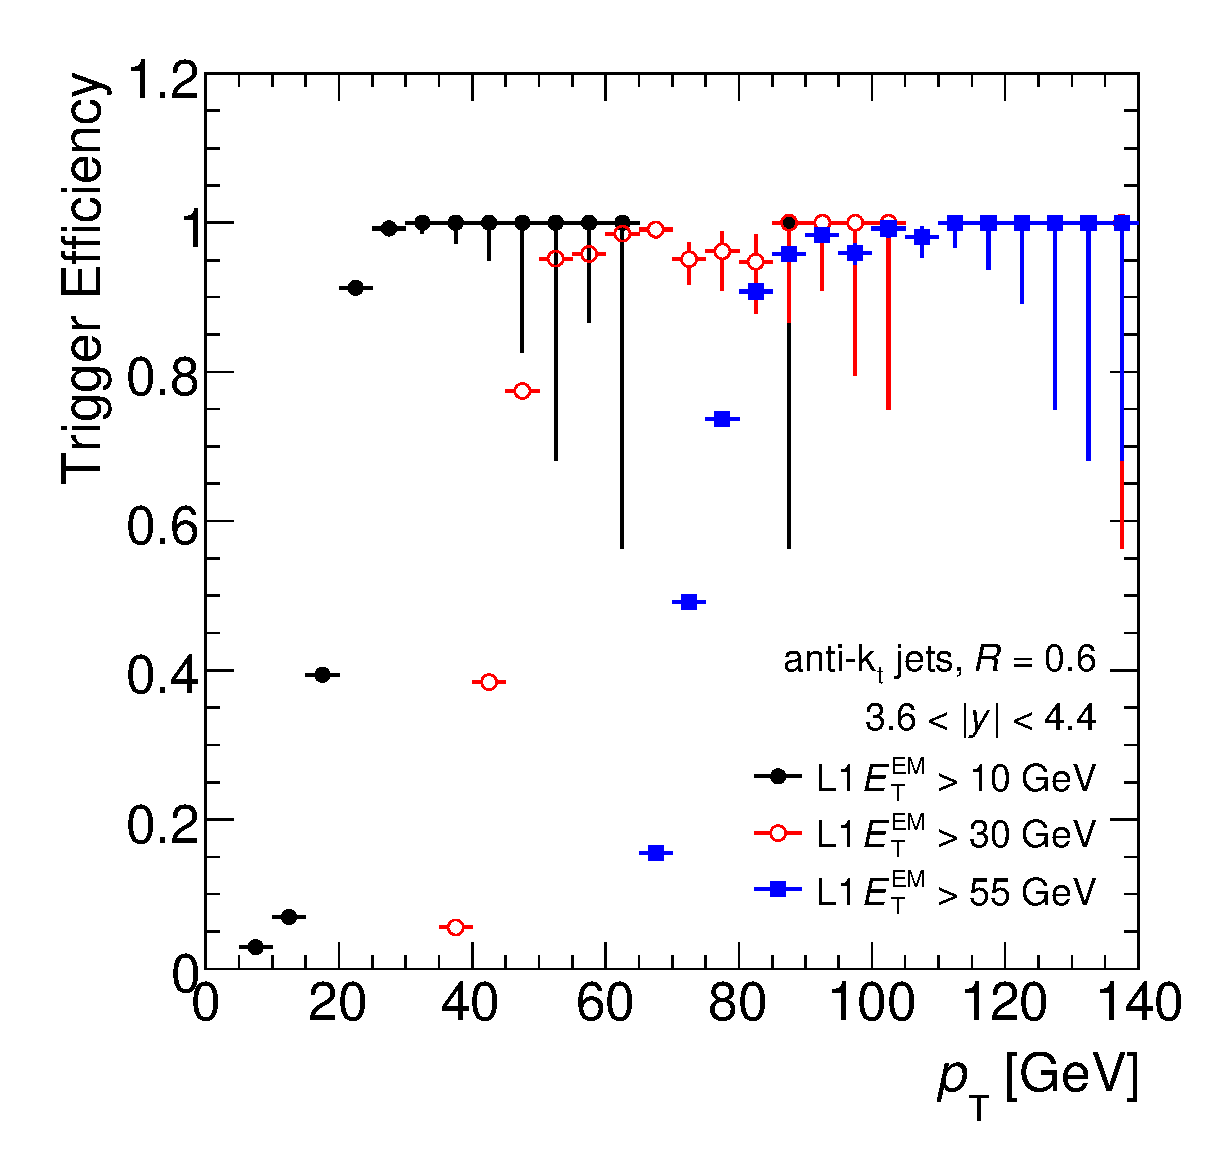
\includegraphics[width=0.45\linewidth,angle=0]{L1_triggers_forward_bin_akt6.eps}
\label{fig_forward6_eff}
}\\
\subfigure[]{
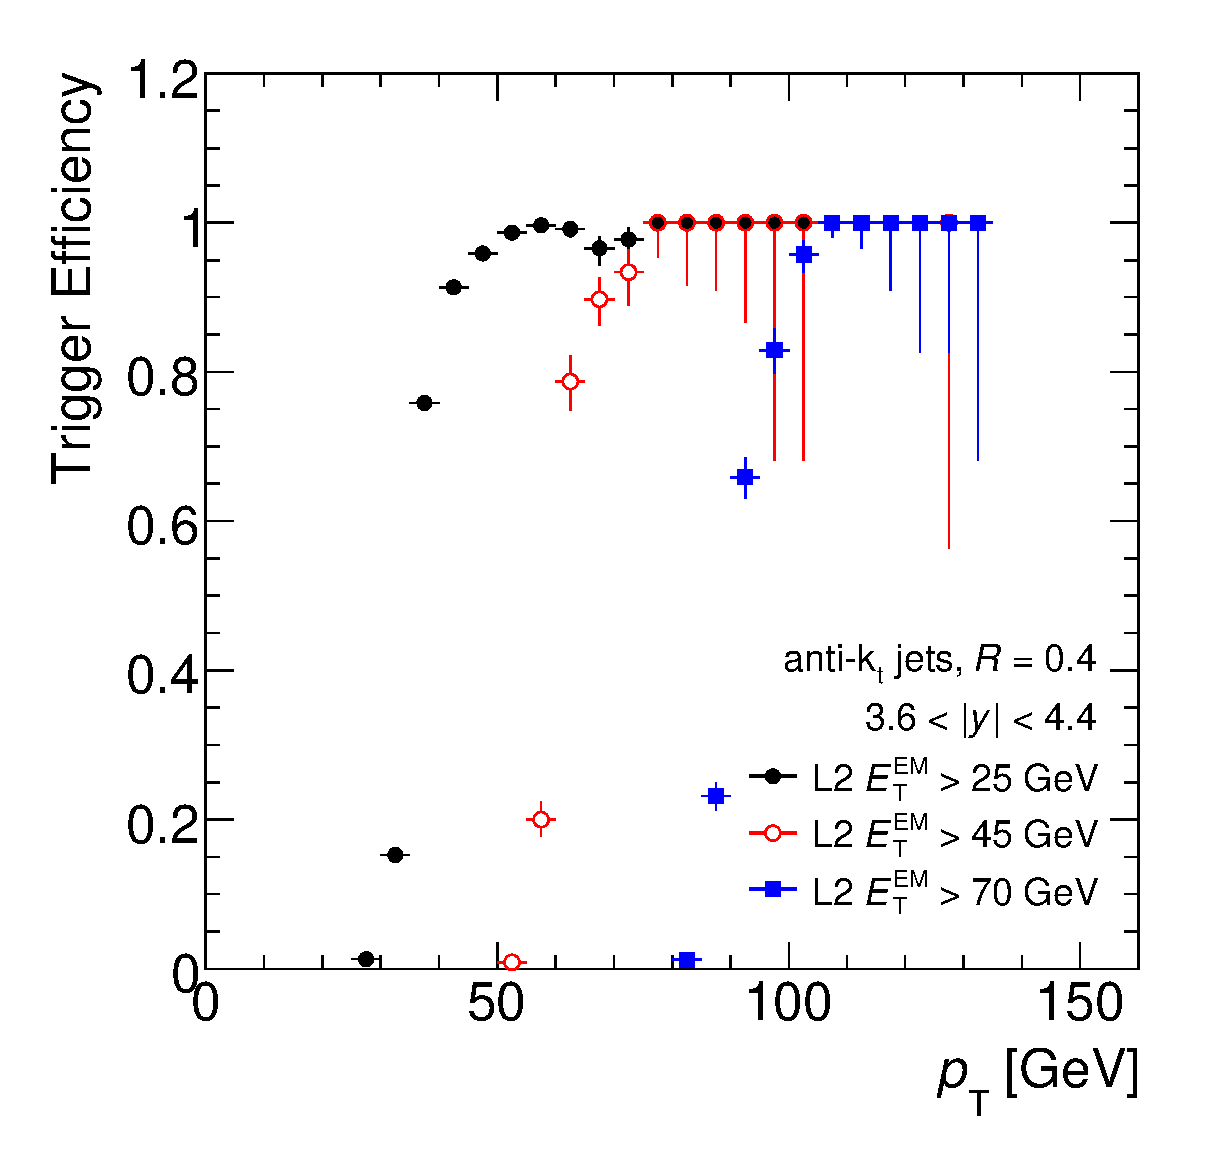
\includegraphics[width=0.45\linewidth,angle=0]{L1L2_triggers_forward_binm_akt4.eps}
\label{fig_forward4_effL2}
}
\subfigure[]{
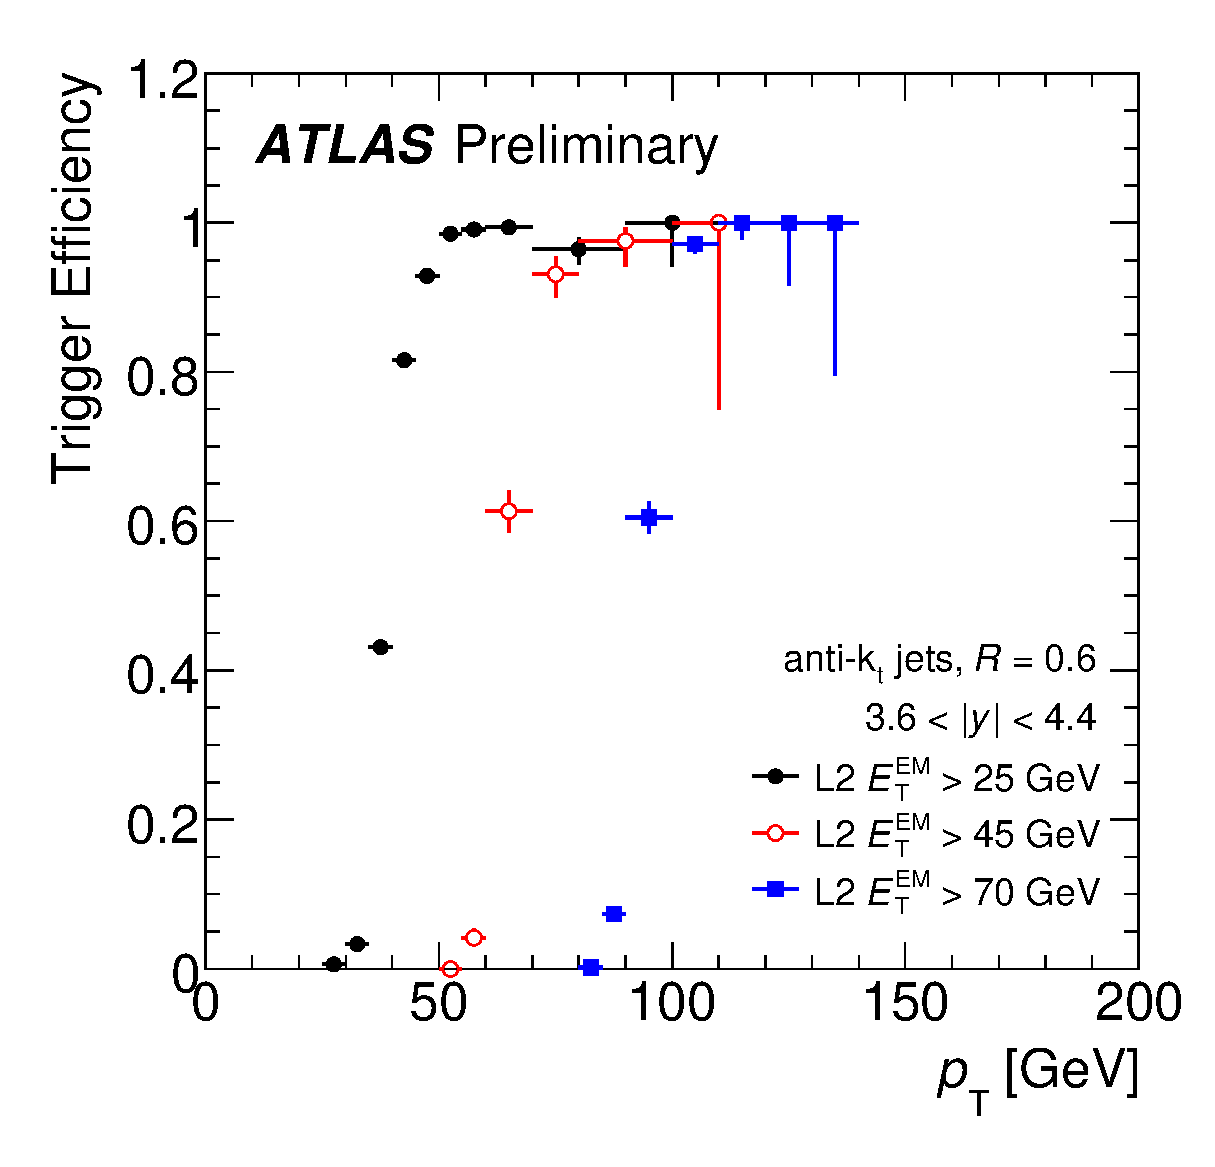
\includegraphics[width=0.45\linewidth,angle=0]{L1L2_triggers_forward_binm_akt6.eps}
\label{fig_forward6_effL2}
}
\caption[Trigger efficiencies in the forward bin]{Efficiencies for  L1 triggers (top) and L2 triggers (bottom) in the forward bin, for \akt jets with R=0.4 (left) and R=0.6 (right).} 
\label{figures_forward}
\end{centering}
\end{figure}

\begin{figure}[tbp]
\begin{centering}
\subfigure[]{
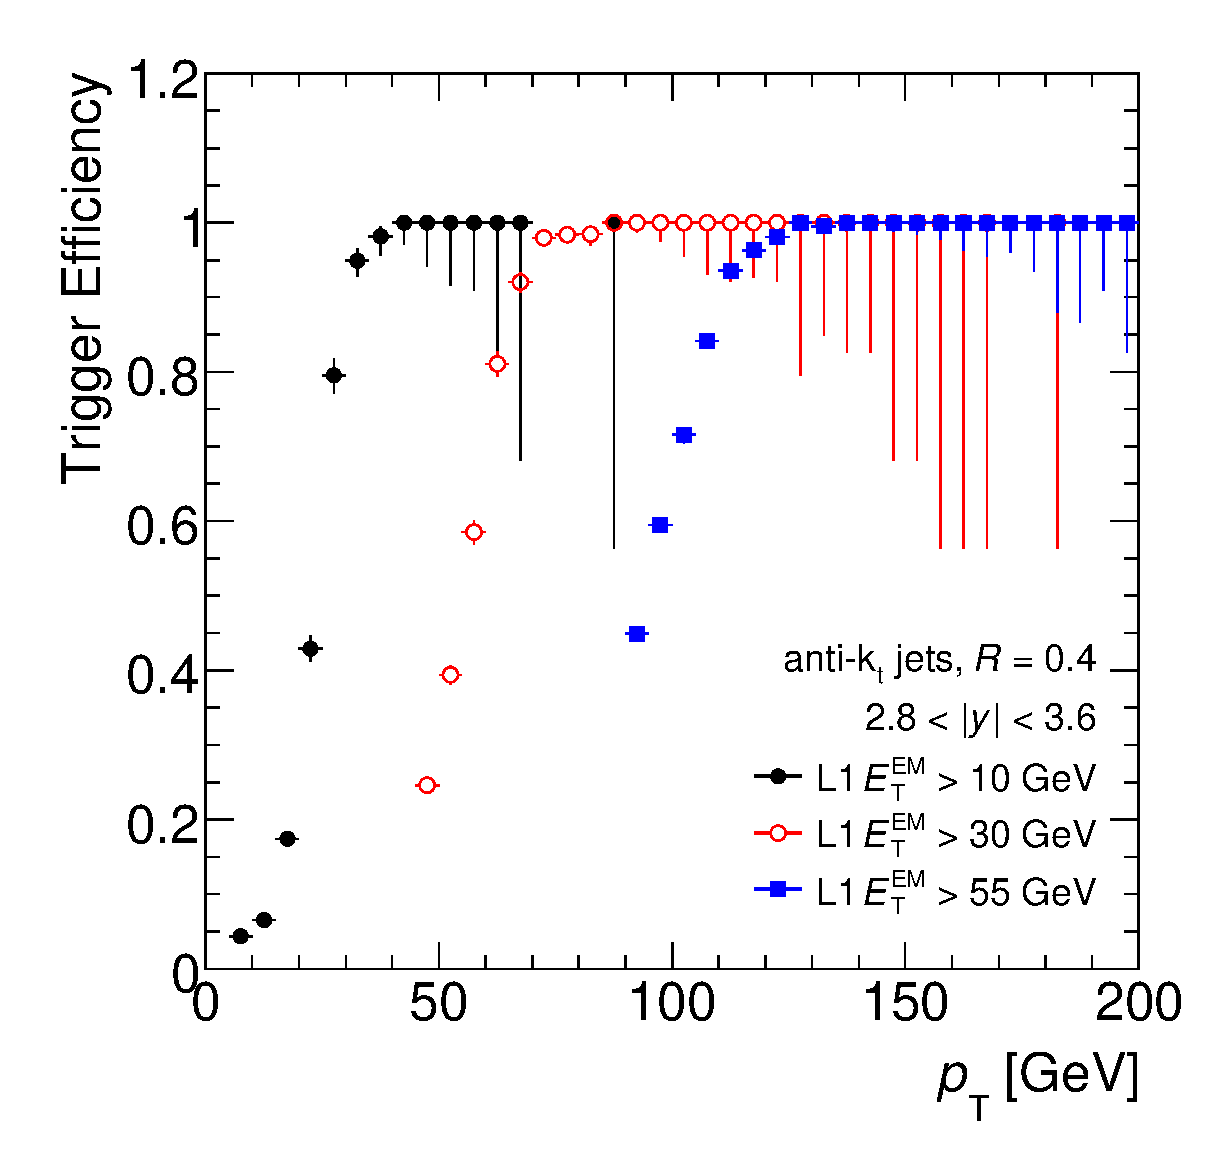
\includegraphics[width=0.45\linewidth,angle=0]{L1_triggers_transition_bin_akt4.eps}
\label{fig_trans4_eff}
}
\subfigure[]{
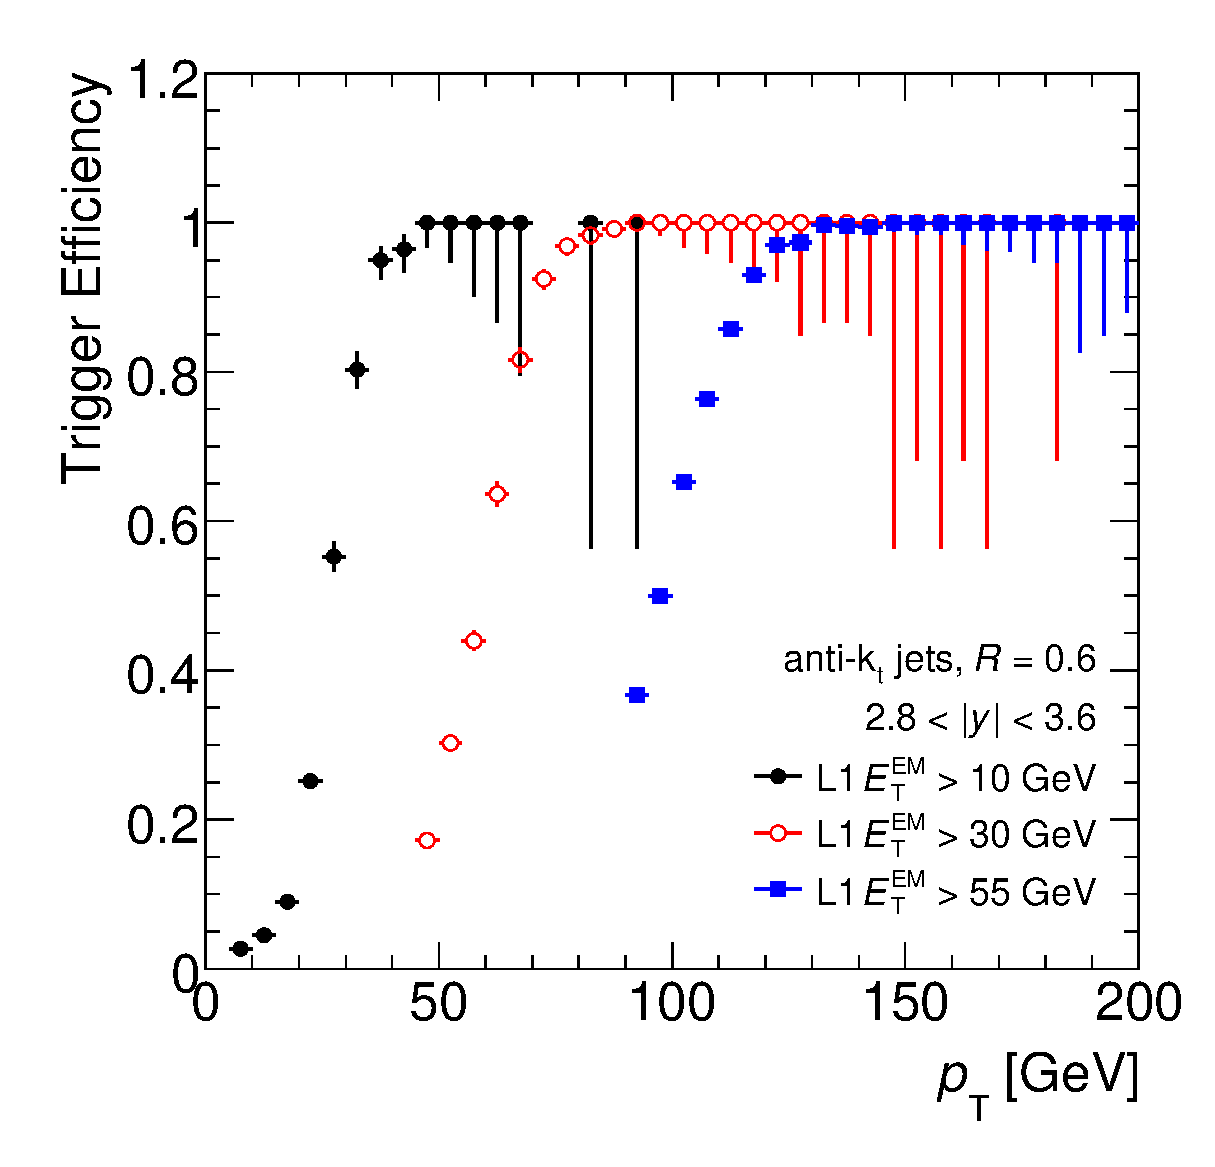
\includegraphics[width=0.45\linewidth,angle=0]{L1_triggers_transition_bin_akt6.eps}
\label{fig_trans6_eff}
}\\
\subfigure[]{
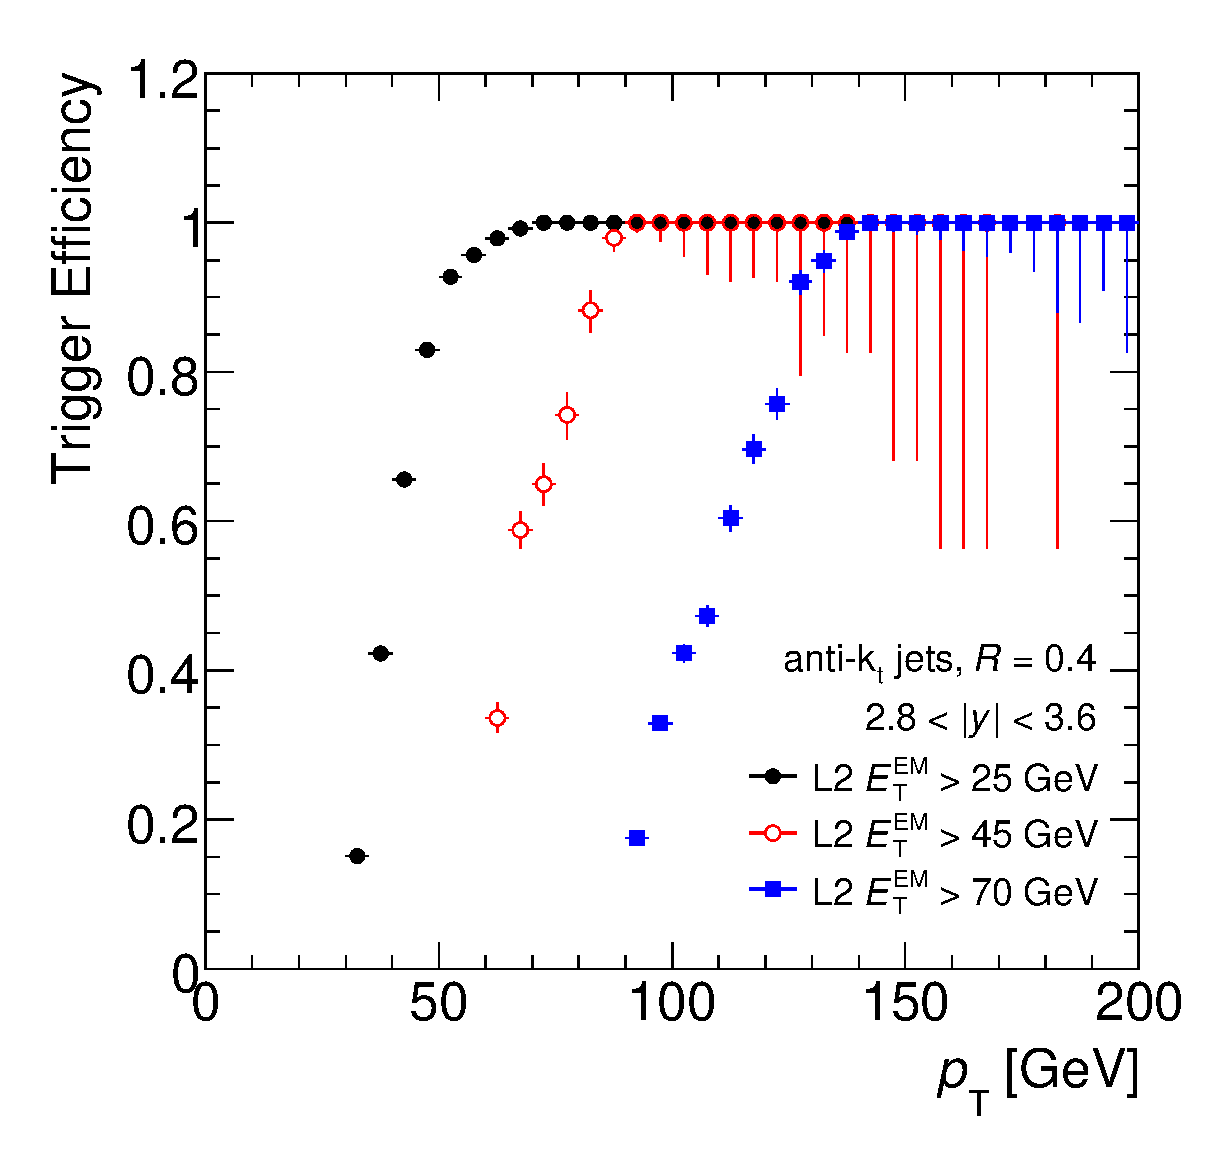
\includegraphics[width=0.45\linewidth,angle=0]{L1L2_triggers_transition_binm_akt4.eps}
\label{fig_trans4_effL2}
}
\subfigure[]{
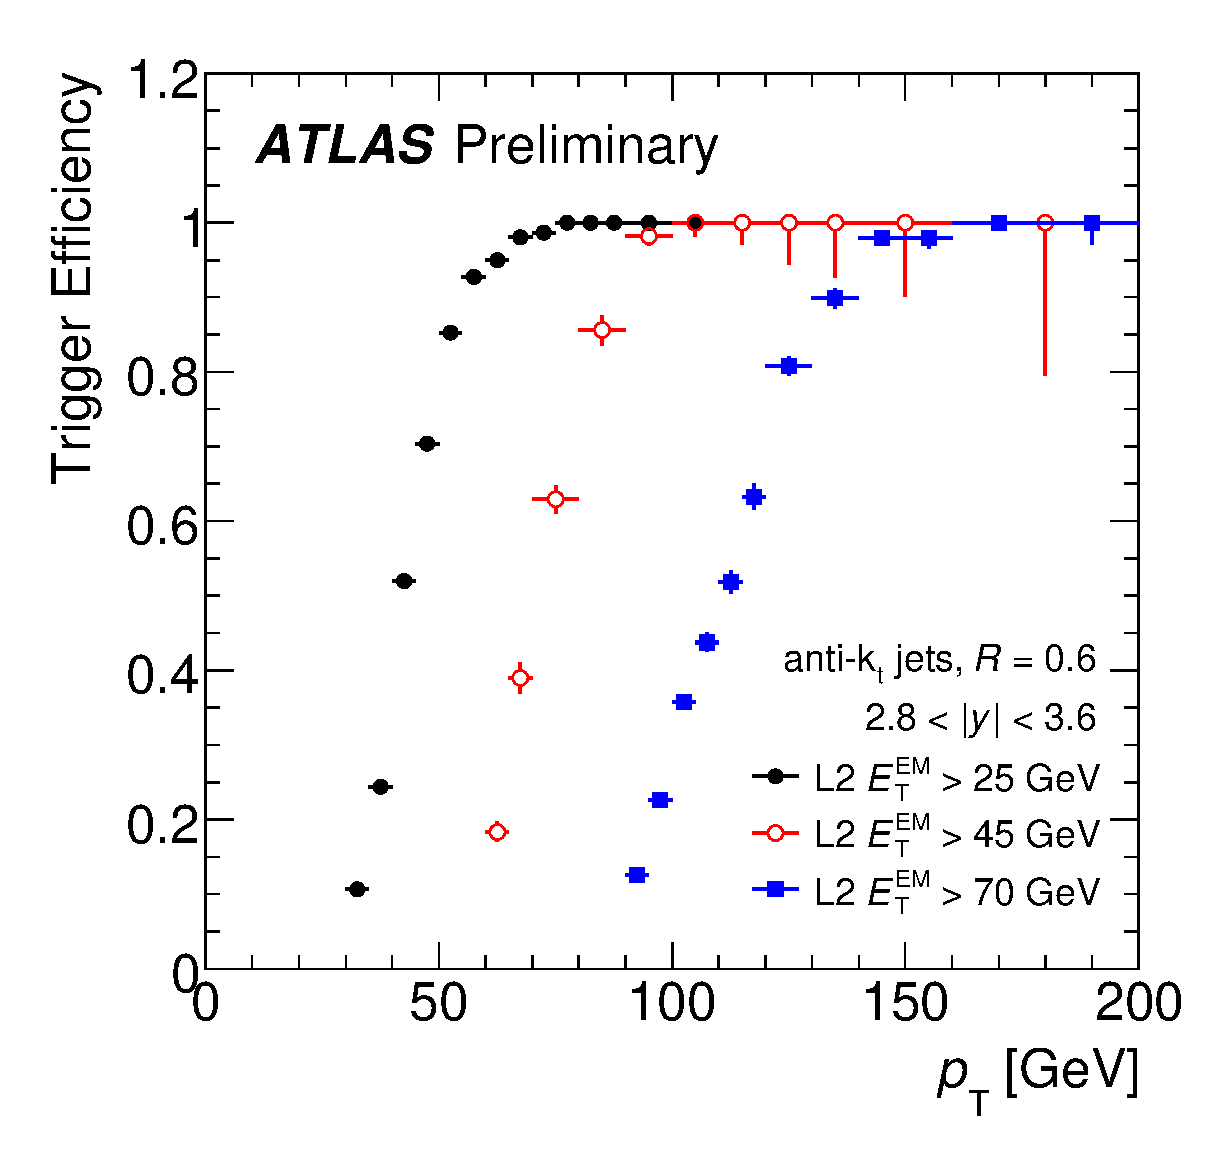
\includegraphics[width=0.45\linewidth,angle=0]{L1L2_triggers_transition_binm_akt6.eps}
\label{fig_trans6_effL2}
}
\caption[Trigger efficiencies in the transition bin]{Efficiencies for L1 triggers (top) and L2 triggers (bottom) in the transition bin, for \akt jets with R=0.4 (left) and R=0.6 (right).} 
\label{figures_trans}
\end{centering}
\end{figure}
% Trigger commissioning continued as data taking progressed during 2010. Initially only the L1 trigger was active, although for the later periods with higher luminosity the HLT was incorporated into the trigger decision. For periods G through I level 2 trigger algorithms were used to select events. 



% When the trigger system detects a jet with Et above some threshold, it will pass the event. However, as the detector has a nonzero resolution, jets will be mis-measured by some amount. Because of this, the 
%
%For the three lowest \pt~bins, the MBTS trigger is used to collect data at all rapidities. 



\subsection{Trigger strategy for the Transition Bin}
\label{section_transbin}
The transition bin covers the difficult region between the end-cap calorimeters and the FCal. The central jet trigger only uses information from the EMEC and HEC (which covers the region $|\eta|< 3.2$), while information from the FCal is only used by the forward jet trigger ($|\eta| > 3.2)$. Note that as jets have a finite radius, jets in the transition region may deposit energy in both the FCal and in the EMEC/HEC. Thus, in order for the analysis to be sensitive to all jets in this region of rapidity, both the central and forward jet triggers need to be considered when collecting data. This is done by taking the logical ``OR'' of the two triggers, such that jets in the event are counted if either the central or forward trigger condition is met. The per-jet efficiency of each trigger throughout this rapidity range is shown in Figure~\ref{fig_transbin_rapidity_coverage}. The ``OR'' of the two triggers is fully efficient throughout the rapidity range of the transition bin, although the individual triggers are not. 

\begin{figure}[tb]
\centering 
\subfigure{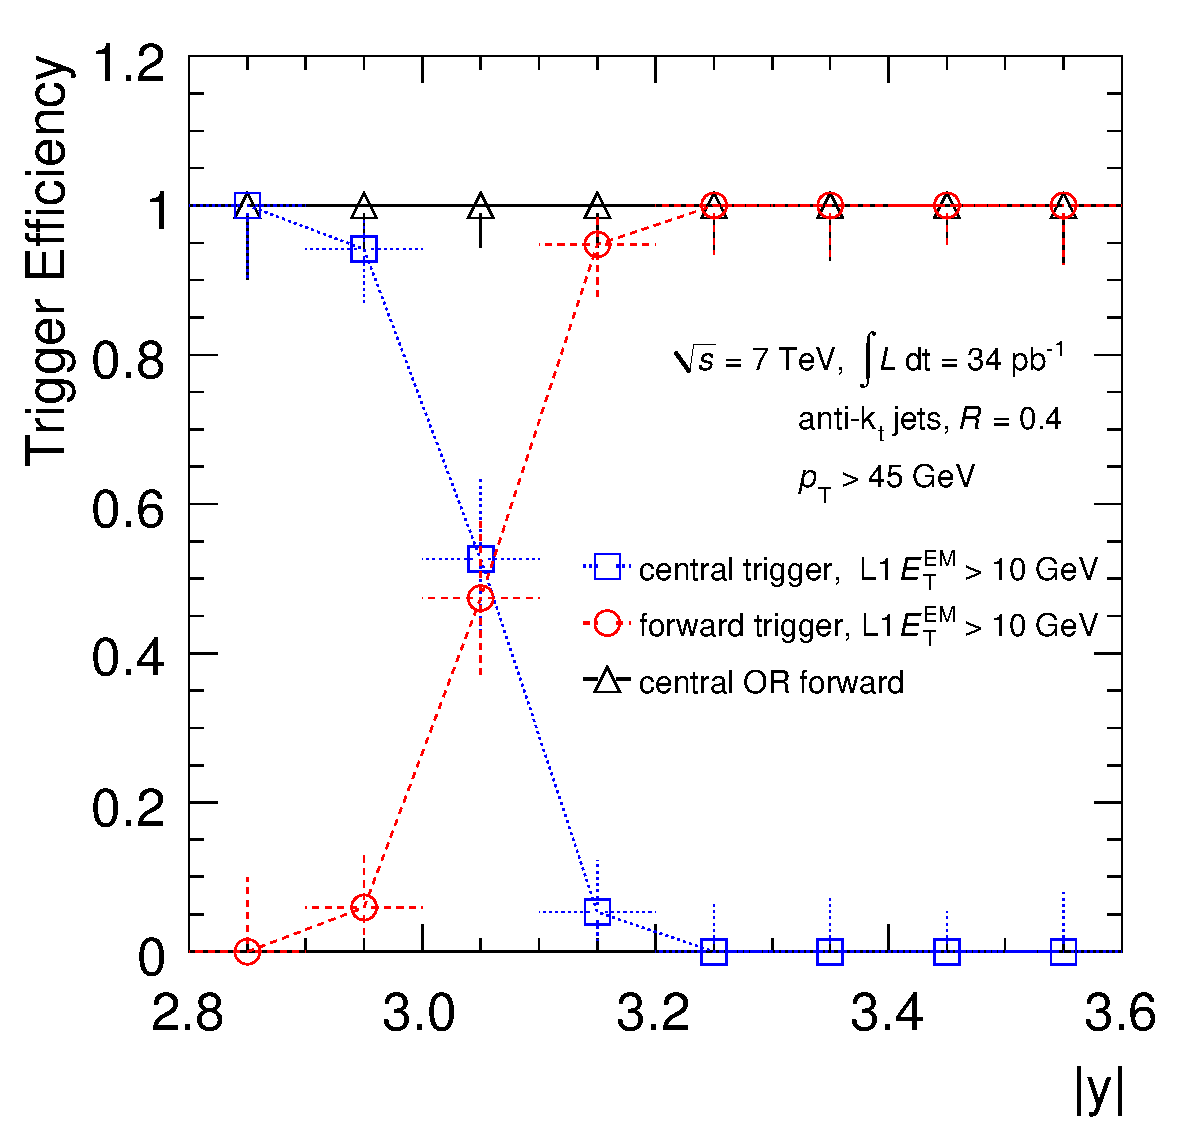
\includegraphics[width=0.45\linewidth]{eta_efficiency_akt4}}
\subfigure{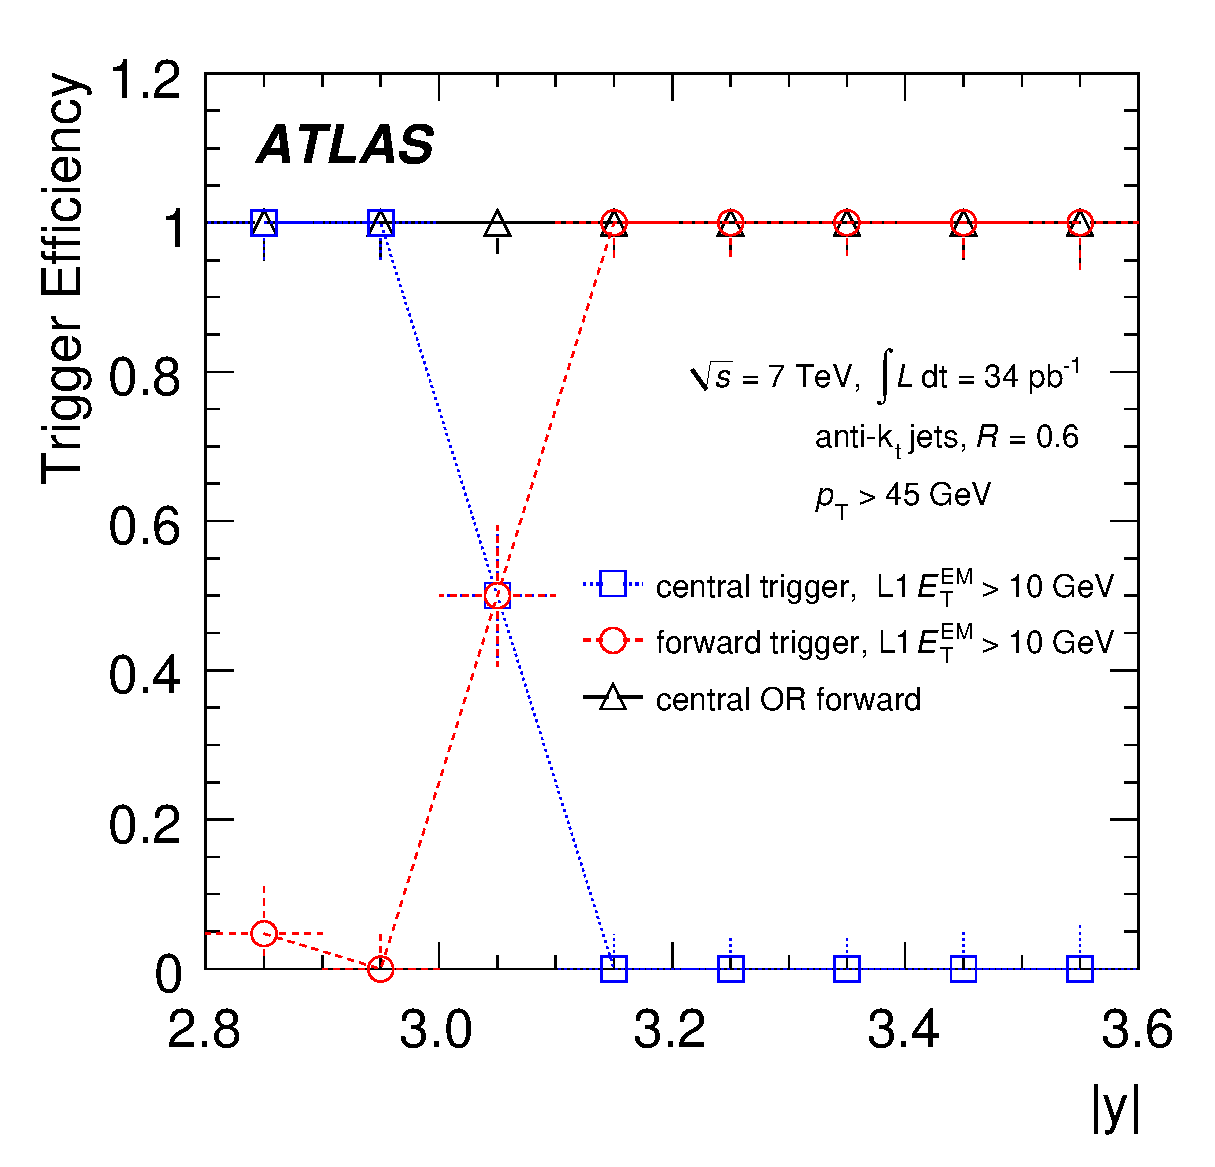
\includegraphics[width=0.45\linewidth]{eta_efficiency_akt6}}
\caption[Trigger efficiency vs. $y$]{Per-jet efficiency of Level 1 forward (red) and central (blue) jet triggers as a function of jet rapidity for jets with \pt~$>$ 45 GeV in the transition bin ($2.8 < |y| < 3.6$), for jets with $R$ = 0.4 (a) and $R$ = 0.6 (b). Note that the OR of the two triggers remains fully efficient throughout the rapidity range.}
\label{fig_transbin_rapidity_coverage}
\end{figure}

When only a single trigger is used, the measured cross-section is given by
\begin{equation}
%\sigma = \frac{N_{jets}}{\intL /S},
\sigma = N_{jets}\left(\sum_i\frac{\intL_i}{S_i}\right)^{-1},
\end{equation}
where $N_{jets}$ is the number of jets observed and $\intL_i$ and $S_i$ are the integrated luminosity and trigger prescale for the $i$th luminosity block, respectively.\cmt{is the integrated luminosity seen by the detector} The situation is more complex in the case where two triggers are employed~\cite{combining_triggers}. In this situation events are classified as belonging to one of three classes, based on whether the event passed the forward trigger condition but not the central (case 10), the central trigger condition but not the forward (case 01), or both trigger conditions (case 11). When making these distinctions, it is important to consider whether the event satisfied a trigger condition before the prescale was applied, as events should be classified according to the triggers that they could potentially be accepted by rather than the triggers that actually selected the event. For L1 triggers the ``Trigger Before Prescale'' flag can be checked in \athena, but for L2 triggers the jets found at L2 must be checked to see if any exceed the trigger threshold.

Once the events have been divided into their respective classes, the cross-section may be written as \begin{equation}
\sigma =  \frac{N_\mathrm{01}}{\intL_\mathrm{01}} + \frac{N_\mathrm{10}}{\intL_\mathrm{10}} +\frac{N_\mathrm{11}}{\intL_\mathrm{11}},
\end{equation}
where the integrated luminosities are given by
%\begin{equation}
%\intL_\mathrm{01(10)} = \sum_i\frac{\intL_i}{S_i\mathrm{,01(10)}}\right)^{-1}
%\end{equation}
\begin{eqnarray}
\intL_\mathrm{01} &=& \sum_i\frac{\intL_i}{S_{i\mathrm{,01}}}\\
\intL_\mathrm{10} &=& \sum_i\frac{\intL_i}{S_{i\mathrm{,10}}}\\
\intL_\mathrm{11} &=& \sum_i\frac{\intL_i \left(S_{i\mathrm{,01}} + S_{i\mathrm{,10}} - 1\right) }{ S_{i\mathrm{,01}} \, S_{i\mathrm{,10}}}
\end{eqnarray}
where $S_{i\mathrm{,10}}$ ($S_{i\mathrm{,01}}$) is the prescale of the forward (central) jet trigger for the $i$-th lumiblock.



%Add Dijets in here
% use paper for unfolding/results
% talk about dijet triggers - talk about work I did - initially were going to use y_max, switched to delta_y, because...


\subsection{Dijet Triggers}

For the initial measurements made using data from \atlas \cite{InclusivePaperAtlas1,inclusive_confnote_1} the dijet mas spectrum was binned in terms of the dijet mass, \mass, and the maximum rapidity of the two jets, $y_\mathrm{max} = \max (|y_1|,|y_2|)$. Dijet events were selected by triggering on the leading jet, using the same trigger thresholds as for inclusive analysis. These first measurements only considered cases where both jets were in the central region, with $y_\mathrm{max} < 2.8$.

For extension of the dijet analysis to the transition and forward regions, a new trigger scheme was initially considered. The intent was to bin the trigger efficiency in terms of the observables of interest. The central jet trigger would be used for $y_{max} < 2.8$, the forward jet trigger for $3.6 < y_{max} < 4.4$, and the OR of the two for $2.8 < y_{max} < 3.6$, with the trigger efficiency being described by a turn-on curve in \mass. Each trigger could then be considered fully efficient above some threshold value for the dijet mass, and used to collect data above this point. 
This trigger scheme was later abandoned, as the trigger system is based on jet \pt~and thus  inflates the minimum dijet mass at which the trigger becomes unbiased.
Consider the case where both jets in the dijet system have transverse momenta well above the trigger threshold, but the separation between jets is small. The small separation between jets will yield a small mass, and the trigger will efficiently accept dijet events in this configuration.
However, in cases where the separation between jets is large and the jet momenta are close to the trigger threshold, the resulting value for the dijet mass can still be quite large while the trigger is not fully efficient. 
%
For this reason, the observables of interest were changed to $m_{12}$ and half of the jet rapidity separation\footnote{In the parton-parton centre of mass frame, the scattered partons each have \pt = $m_{12}/\mathrm{cosh}(y^*)$ and rapidity $\pm y^*$. For this reason $y^*$ is considered a more desirable variable than $y_\mathrm{max}$.}, $y^* = |y_1 - y_2|/2$. The  trigger scheme then reverted back to that used for earlier versions of the analysis wherein the leading jet was used to trigger the event, although this was extended to cover the forward and transition regions. The L1 trigger efficiencies obtained when using this method are plotted in Figures~\ref{trig_dijet_L1_T} and \ref{trig_dijet_L1_F}, for the transition bin and forward bin respectively, and are plotted as a function of the leading jet \pt. The trigger scheme was then expanded to consider the subleading jet, utilising a method similar to that used for the transition bin in the inclusive analysis. The kinematic region was divided into a number of bins in \pt~and rapidity, each of which was associated with a trigger threshold.  Events were then divided into categories based on whether the trigger condition associated with the leading jet was met, or that for the subleading jet, or if both trigger conditions were satisfied. As there is some overlap between the forward and central jet triggers for jets in the region $3.0 < |y| < 3.2$ (Figure~\ref{fig_transbin_rapidity_coverage}), jets in this region were matched to ROIs at L1 or trigger jets at L2 in order to determine whether the jet should be associated with the forward or central trigger. Events are then weighted based on the prescales of the triggers, using a generalised version of the method described in Section~\ref{section_transbin}, in order to account for the larger number of trigger categories.

\begin{figure}[tbp]
\subfigure{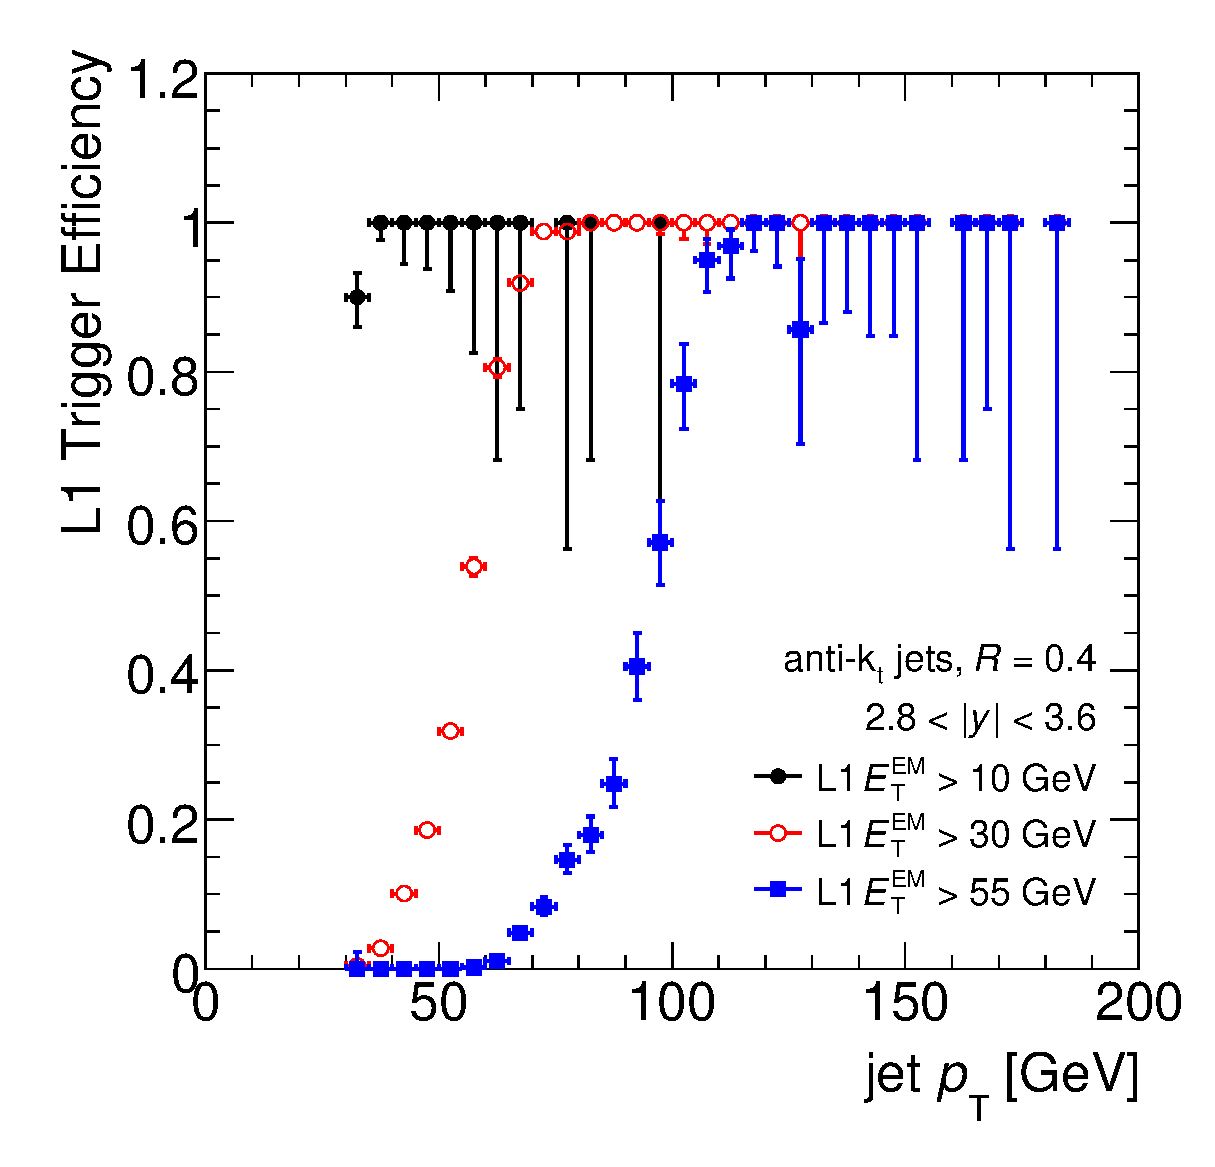
\includegraphics[width=0.45\linewidth,angle=0]{my_dijet/L1_T4.eps}}
\subfigure{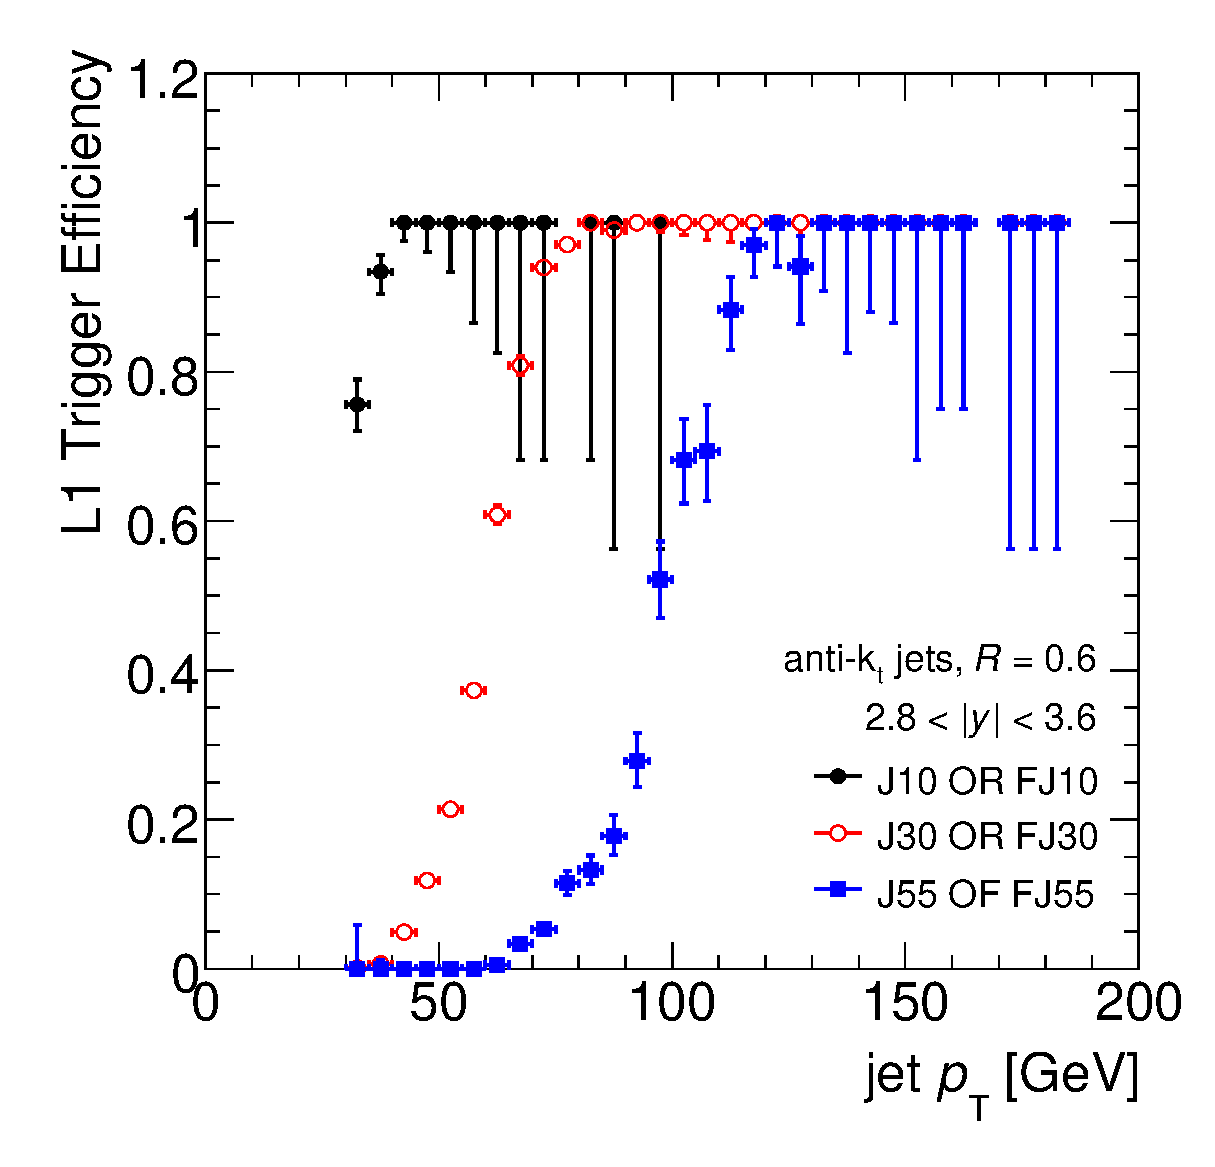
\includegraphics[width=0.45\linewidth,angle=0]{my_dijet/L1_T6.eps}}
\caption[Dijet trigger efficiency, transition bin]{L1 trigger efficiencies for dijet events in which the leading jet lies in the transition bin, for \akt jets with $R=0.4$ (left) and $R=0.6$ (right).}
\label{trig_dijet_L1_T}
\end{figure}

\begin{figure}[tbp]
\subfigure{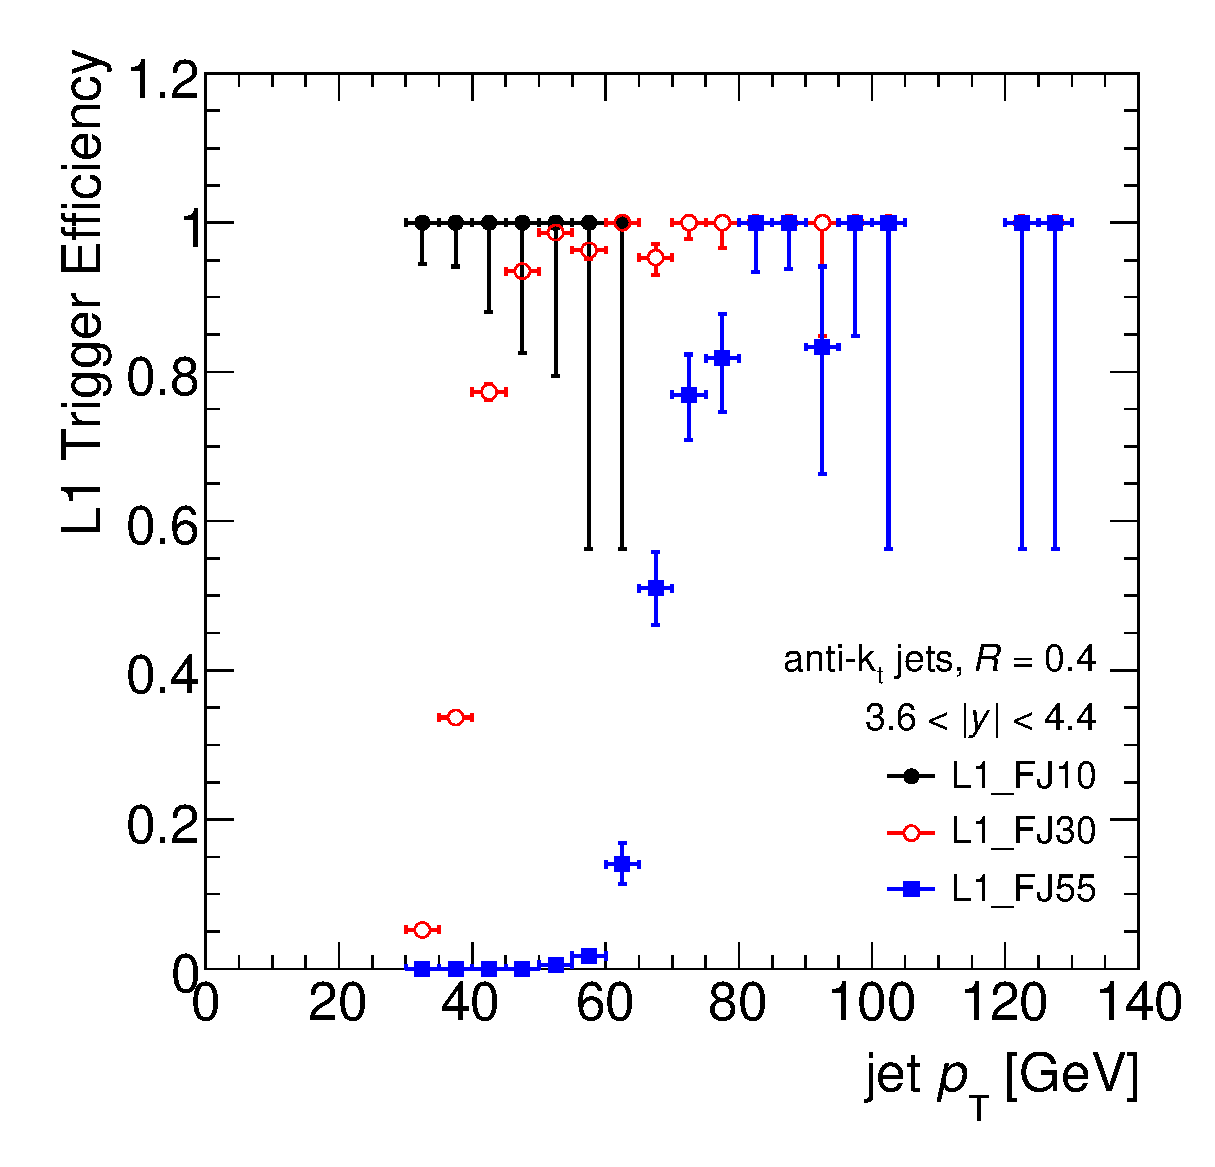
\includegraphics[width=0.45\linewidth,angle=0]{my_dijet/L1_F4.eps}}
\subfigure{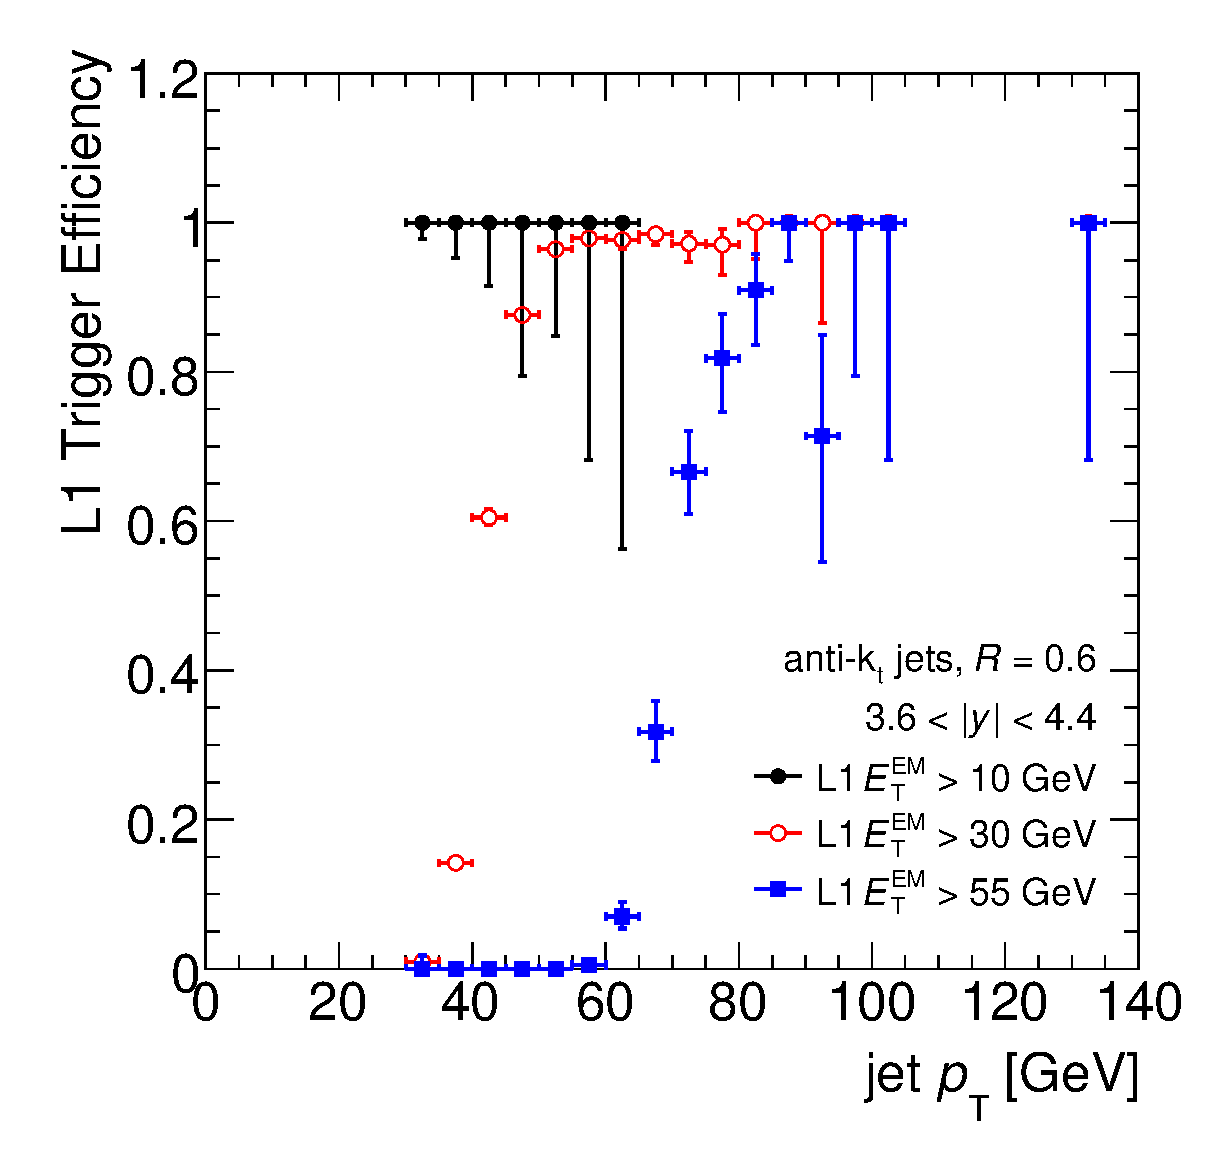
\includegraphics[width=0.45\linewidth,angle=0]{my_dijet/L1_F6.eps}}
\caption[Dijet trigger efficiency, forward bin]{L1 trigger efficiencies for dijet events in which the leading jet lies in the forward bin, for \akt jets with $R=0.4$ (left) and $R=0.6$ (right). Note that the 10 GeV trigger threshold is alwasy satisfied by the leading jet as dijet events are required to have a leading jet with \pt~$>$ 30 GeV, which is greater than the plateau point for the 10 GeV trigger threshold.}
\label{trig_dijet_L1_F}
\end{figure}






 
 






%transition bin complicated as it covers the region of rapidity between the HEC and FCAL.
%
%pic of cross-section
%plot showing per jet efficiency
%talk about the or
%talk about cross-section measurement.


%\label{IncJets_transbin}
\section{Unfolding}
\label{sec::unfolding}
 % unfolding
\cmt{
after cross-section calculations are carried out in Section above, data needs to be corrected in order to account for (acceptance) and detector effects

done using Monte Carlo, matching truth and reco to obtain a folding matrix A

inverting matrix bad if condition number is not close to one/ negative correlations between bins.

for small eigenvalues, corresponding components (and their stat. fluctuations) magnified  by 1/lambda. This produces large fluctuations in unfolded spectrum. unfolded spectrum dominated by a few components with small evalues and large statistical errors, not good.

Solution dominated by components with large (small?) eigenvalues. with eigenvalues not close to one, small statistical fluctuations are magnified leading to solution that is not smooth, undesirable.

small coefficients tend to correspond to high frequency components, i.e. rapid oscillations from bin to bin. These are the ones most affected by statistical fluctuations, 
}



After the cross-section calculations have been carried out as described above, the data need to be corrected for acceptance and detector effects before it can be compared to any theoretical predictions. As the jet cross-section falls sharply with \pt, the non-zero resolution of the detector causes the measured spectrum to be skewed towards higher \pt~relative to the ``true'' spectrum. Monte Carlo may be used to compare the \pt~of truth jets with reconstructed jets in order to understand the effects of the detector resolution. These effects can then be ``unfolded'' from the measured spectrum in order to obtain the spectrum of jets prior to their interaction with the detector.

%that is, infer the spectrum of jets 

%Simplest method is bin by bin, not great if there are large fluctuations or correlations

Information on detector related effects is contained in the transfer matrix, $A_{ij}$, which describes the influence that detector effects have on the measured results, and must be derived from simulation. The entry $A_{ij}$ is equal to the number of truth jets in the $j$-th \pt~bin which are reconstructed in the $i$-th \pt~bin.  This may be normalised to produce the folding matrix of probabilities, $P_{ij}$, given by
\begin{equation}
P_{ij} = \frac{A_{ij}}{\sum_{k=0}^{N_b} A_{kj}}
\end{equation}
The spectrum at truth level, $t_j$, and the reconstructed spectrum $r_j$, are then related by
\begin{equation}
r_j = \sum_{k=0}^{N_b} P_{jk} t_k.
\end{equation}
An unfolded result, $u_j$, may then be obtained from the measured data $d_j$, by solving the matrix equation
\begin{equation}
d_j = \sum_{k=0}^{N_b} P_{jk} u_k.
\label{eqn_fold_1}
\end{equation}
The solution to this may be found by inverting $P_{ij}$, such that $u_j = \sum_k P^{-1}_{ik} d_k$. However, this is undesirable as it yields large fluctuations in $u_j$ \cite{Blobel:2002pu}. Transfer matrices tend to have large condition numbers, meaning that the solution is sensitive to slight changes in the input. Small variations in $d_j$, which may be due to statistical fluctuations, can produce large spurious fluctuations in $u_j$. 

In order to avoid this, the unfolding method must incorporate some form of regularisation. Typically equation~\ref{eqn_fold_1} is solved numerically, and regularisation may be done, for example, by incorporating the smoothness of $u_j$ into the optimisation method \cite{Blobel:2002pu}. In this analysis, the unfolding is carried out using the Iterative, Dynamically Stabilised (IDS) method \cite{Malaescu:2009dm,Malaescu:2011yg}, which is described below. \cmt{\blue{successively reweight Mont Carlo to better match data}}

\subsection{The Iterative, Dynamically Stabilised Unfolding Method}
%Consider the case where the reconstructed MC matches the measured data exactly. In this (unlikely) %scenario, the truth level MC could be taken as the unfolded data.

In the IDS method, the MC is re-weighted at each iteration such that the reconstructed MC spectrum is brought closer to that of the measured data, with the truth level spectrum and the transfer matrix adjusted accordingly. As the reconstructed MC is brought closer to the measured data spectrum through re-weighting, the truth level spectrum approaches the desired unfolded result. Any differences between the measured data spectrum and the reweighted reconstructed MC spectrum are then unfolded.
%For features present in the measured data which were not simulated by the MC, the difference between data and reconstructed MC is then unfolded.

\cmt{In the IDS method, the r}Regularisation is implemented through the use of a regularisation function, $f(\Delta x,\sigma,\lambda)$. This function determines how much unfolding should be carried out in a given iteration based on the difference between data and Monte Carlo, $\Delta x$, the uncertainty in this difference, $\sigma$, and a regularisation parameter $\lambda$. The regularisation function should take the ratio $\Delta x/\sigma \lambda$ as an argument, and return a value near zero at small values of this argument and approach one at higher values. \cmt{There are many types of function which meet these criteria, some of which are plotted \red{below}.}  

As the regularisation function depends on the difference between data and Monte Carlo, it is important that the Monte Carlo be normalised appropriately. The discrepancy is defined as 
\begin{equation}
\Delta d_k = d_k - \frac{N_{\mathrm{dSmc}}}{N_\mathrm{MC}} r_{k}
\end{equation}
where $N_\mathrm{MC}$ is the total number of jets in the MC sample and $N_{\mathrm{dSmc}}$ is the number of jets in the data spectrum that correspond to structures/shapes present in the MC spectrum. Normalising the MC in this way enables the unfolding to preserve features in the data, such as new physics signals, which were not simulated in the MC, while correctly scaling the MC in regions where it has a similar shape to the data. The total number of jets in the data sample may be taken as an initial estimate for $N_{\mathrm{dSmc}}$. A better estimate may then be obtained using

\begin{equation}
N_{\mathrm{dSmc}}^\prime = N_{\mathrm{dSmc}} + \sum_{k=1}^{N_B} \left ( 1 - f\left(\Delta d,\sigma,\lambda \right )\right) \Delta d_k .
\label{unfold_norm_eq}
\end{equation}
This procedure may be repeated until the relative change in $N_{\mathrm{dSmc}}$ is less than a desired threshold.

%\red{uncertainty on $d_k$}


\subsection{Matching Efficiency}
In order to obtain the transfer matrix from the Monte Carlo, reconstructed jets need to be matched with a corresponding truth jet. Jets are matched if they lie within a distance $\Delta R < 0.3$ in $y-\phi$ space. The spectrum of matched truth (or reconstructed) jets may be obtained by projecting the transfer matrix onto the appropriate axis. The matched spectrum may then be compared to the unmatched spectrum to obtain the matching efficiency for truth jets and for reconstructed jets. As the transfer matrix is derived using only matched pairs of jets, the effect of the matching efficiency should be taken into consideration. Prior to the unfolding, the measured data is multiplied by the matching efficiency for reconstructed jets, and after unfolding the result is divided by the matching efficiency for truth jets. 


%A similar difference, $\Delta u_k$, may be defined for the unfolded data at an intermediate iteration:
%\begin{equation}
%\Delta u_k = u_k - \frac{N_{\mathrm{dSmc}}}{N_\mathrm{MC}} t_{k}.
%\end{equation}

 
 
% For the measured data, the difference is taken with respect to the reconstructed MC, whereas for the unfolded data the difference is with respect to MC at the truth level.
 
 
 
An initial unfolding may then be performed on the data, yielding the result
\begin{equation}
u_j =  t_j \cdot \frac{N_{\mathrm{dSmc}}}{N_\mathrm{MC}} + \left [1 - f\left ( \Delta d_k, \sigma d_k, \lambda_M\right )\right ] \cdot \Delta d_j  + \sum_{k=1}^{N_B} f\left ( \Delta d_k, \sigma d_k, \lambda_M\right ) \cdot  \tilde{P_{kj}} \cdot \Delta d_k 
\label{unfold_unfolding_eq}
\end{equation}
where the unfolding matrix $\tilde{P_{ij}}$ is obtained from the transfer matrix:
\begin{equation}
\tilde{P_{ij}} = \frac{A_{ij}}{\sum_{k=0}^{N_b} A_{ik}}
\end{equation}
The regularisation functions determine how much unfolding is done in a given bin, based on the regularisation parameter $\lambda$ and significance of $\Delta d_k$. Only the difference between measured data and reconstructed MC is unfolded: in bins where $\Delta d_k$ is small, the unfolded result is dominated by the truth level MC spectrum. In those bins where the discrepancy is significant, the regularisation parameter $\lambda$ determines how much unfolding is carried out. For larger values of $\lambda$, less unfolding is performed on the data. 

Once an initial estimate of $u_j$ has been obtained, this may be used to reweight the MC at truth level, and thus improve the transfer matrix. The updated transfer matrix is given by
\begin{equation}
A^\prime_{ij} = A_{ij} + f(|\Delta u_j|, \sigma u_j, \lambda) \cdot \frac{N_\mathrm{MC}}{N_\mathrm{dSmc}} \cdot P_{ij} \cdot \Delta u_j, 
\end{equation}
where 
\begin{equation}
\Delta u_j = u_j - \frac{N_{\mathrm{dSmc}}}{N_\mathrm{MC}} \cdot t_{j}.
\end{equation}
 The new transfer matrix can then be used to update the folding and unfolding matrices, $P_{ij}$ and $\tilde{P}_{ij}$. The procedure may then be carried out iteratively in the following sequence:
\begin{itemize}
\item Update the normalisation factor, $N_\mathrm{dSmc}$, according to~\ref{unfold_norm_eq};
\item Perform the unfolding;
\item Use the unfolded data to update the transfer matrix, and the folding/unfolding matrices.
\end{itemize}


\cmt{ things left to do for unfolding:

say something about uncertainties, sigma dj, sigma uj. When do we stop unfolding?
add plot of transfer matrix
discuss matching efficiency
talk about how optimal values of lambda/ number of iterations are obtained.
}


\cmt{ things to do for this chapter:

JES uncertainty
jet selection
event selection / DQ

results and discussion
(can include discussion of MC for comparison in this Section)

dijet stuff. (dijet scale issues can be in results and discussion)

}

\section{Treatment of uncertainties}
\label{sec::uncertainties}
\subsection{Statistical uncertainties}

The statistical uncertainties on the final (unfolded) cross-section measurement are obtained using ``toy'' Monte Carlos. For each toy, Poisson fluctuations are applied to the measured data spectrum and to the transfer matrix. The fluctuated data is then unfolded using the fluctuated transfer matrix. The unfolded spectra from the toys are then used to compute a covariance matrix, from which the statistical uncertainty on the unfolded data is taken.

\subsection{Systematic Uncertainties}

%The uncertainty on the JES has been discussed in Section~\ref{JES_uncertainty_section}.

The JES uncertainty is the dominant source of systematic uncertainty. Its effect on the final cross-section result is found by propagating each of the JES components listed in Section~\ref{JES_uncertainty_section} through the unfolding procedure. 

The uncertainty  on the cross-section associated with a given component is obtained using Monte Carlo. For each rapidity bin of the MC spectrum, a modified spectrum is obtained by shifting the jet \pt~up by one standard deviation of the JES uncertainty component being considered. A second modified spectrum is obtained by shifting jets down in \pt~by the same amount. These modified spectra are then unfolded using the same technique as for data. The relative difference between the modified and nominal spectra (after unfolding) is then taken as the uncertainty on the cross-section associated with this JES component.
%
%The uncertainty on the cross-section associated with this JES component is then taken as the relative difference between the modified and unmodified spectra.
%
%
%
%
%For each rapidity bin, a modified jet spectrum is obtained by shifting all jets up in \pt by one standard deviation of the JES uncertainty component being considered. A second modified spectrum is obtained by shifting jets down in \pt by the same amount. These modified spectra are then unfolded using the same technique as for data. The relative differences between the modified and 
%
%take a rapidity bin
%shift all jets up by 1 sd in pt
%
%
%For each component,
%
%
%done using MC
%
%shift MC up/down, unfold
%relative difference between unfolded shifted spectra and unfolded nominal spectra taken as uncertainty on cross-section.
%
%
% the measured data spectrum is shifted up and down in \pt~by one standard deviation. The shifted spectra are then unfolded, and the uncertainty associated with that component is taken as the difference between the shifted and unshifted spectra, after unfolding.

The effect of the jet energy resolution (JER) uncertainty is propagated through the unfolding in a similar fashion to the JES uncertainty. A modified Monte Carlo sample is produced by smearing the \pt~of the reconstructed jets in the nominal MC sample. The reconstructed jets have their \pt~smeared by a factor $\Delta$, where $\Delta$ is a random variable with standard deviation $\sigma_\Delta$ and a mean of one. The standard deviation of $\Delta$ is chosen to satisfy
\begin{equation}
 \sigma_\Delta^2 + \sigma_{\mathrm{nom}}^2 = \left ( \sigma_{\mathrm{nom}}  + \sigma_\mathrm{JER} \right )^2,
 \end{equation}
where $\sigma_{\mathrm{nom}}$ is the nominal JER and $\sigma_\mathrm{JER}$ is its uncertainty. The additional smearing is thus applied in such a way as to increase the effective JER by one standard deviation. The data are then unfolded using the modified transfer matrix, and the difference between this result and that unfolded with the nominal transfer matrix is taken as the systematic uncertainty. 

The matching between truth and reconstructed jets is another source of systematic uncertainty. As mentioned earlier, the transfer matrix is constructed by matching truth and reconstructed jets within $\Delta R < 0.3$ in rapidity and azimuthal angle. Transfer matrices are also constructed by matching jets within $\Delta R < 0.4$ and $\Delta R < 0.2$. The unfolding is carried out using these matrices, and the largest difference between either result and that obtained from the nominal transfer matrix is taken as the uncertainty.

Shape variations between the MC spectrum and the data will also introduce systematic uncertainties during the unfolding procedure. To estimate this effect, the truth level MC spectrum is reweighted in such a way to improve the agreement between the reconstructed MC and the measured data. The reweighted MC is then unfolded using the original transfer matrix (i.e., the one used to unfold the data). The difference between the result of this \cmt{(reweighted truth MC unfolded with original transfer matrix)} and the reweighted truth level MC is taken as a systematic uncertainty, as it reflects the effect of the MC shape on the unfolded spectrum.

%\red{mention jet reconstruction efficiency in data correction?}
The efficiency with which jets are reconstructed has also been considered. In Monte Carlo, this is equivalent to the matching efficiency. In data, the reconstruction efficiency may be estimated by matching reconstructed jets to track jets, which are formed by running jet-finding algorithms on tracks reconstructed using the inner detector. These two efficiencies may be compared in order to estimate the degree to which the jet reconstruction efficiency is mis-modelled by the simulation. The difference is taken as a systematic uncertainty, and is 2\% for jets with $20 $ GeV $< \pt < 30 $GeV and less than $1\%$ for jets with $\pt > 30$ GeV.

%A plot of the relative systematic uncertainty is shown in Figure~\ref{fig_systematics} systematic for certain rapidity regions is shown in Figure~\ref{fig_systematics}, showing the contributions from various components.
The relative systematic uncertainties for selected rapidity regions are plotted in Figure~\ref{fig_systematics}, showing the contributions from various components. In addition to these components, there is an additional uncertainty of 3.4\% on the cross-section measurements due to the uncertainty associated with the luminosity measurement at \atlas.

%\begin{figure}
%\begin{centering}
%%\subfigure{
%\includegraphics[width=0.3\linewidth,angle=0]{InclusivePtSysIDS_AntiKt06_03_08.eps}
%\includegraphics[width=0.3\linewidth,angle=0]{InclusivePtSysIDS_AntiKt06_21_28.eps}
%\includegraphics[width=0.3\linewidth,angle=0]{InclusivePtSysIDS_AntiKt06_36_44.eps}
%\label{fig_systematics}
%\caption{Systematic uncertainty on the inclusive jet cross-section for \akt jets with $R=0.6$}
%\end{centering}
%\end{figure}
\begin{figure}
\begin{centering}
%\subfigure{
\includegraphics[width=0.3\linewidth,angle=0]{inclusive_results/figs_new/fig_08a_cs_systematic_0_03.eps}
\includegraphics[width=0.3\linewidth,angle=0]{inclusive_results/figs_new/fig_08c_cs_systematic_21_28.eps}
\includegraphics[width=0.3\linewidth,angle=0]{inclusive_results/figs_new/fig_08e_cs_systematic_36_44.eps}
\end{centering}
\caption[Inclusive jet cross-section systematic uncertainty]{Systematic uncertainty on the inclusive jet cross-section for \akt jets with $R=0.6$, for jets in three rapidity regions.}
\label{fig_systematics}
\end{figure}


%BAM!

\section{Results and discussion}
\label{sec::results}
%compared to theory

%\subsection{theoretical predictions}
%
%
%% may not need to mention scales
%Two event generators, NLOJet++ and \powheg, have been used to obtain theoretical predictions for the cross-section at next to leading order (NLO) in perturbative QCD (pQCD). the CT10 PDF set is used as a baseline, although several others (MSTW2008, HERAPDF 1.5, NNPDF 2.1) are considered. 
%For the inclusive jet cross-section, the renormalisation and factorisation scales are both set to the leading jet \pt,
%\begin{equation}
%  \mu_R = \mu_F = p_T^{max}.
%  \end{equation}
%For the dijet results, the cross-section obtained from NLOJet++ was found to be unstable at large values of y^*, yielding negative cross-sections in some cases. Because of this, the scale
%
%\begin{equation}
% \mu_R = \mu_F = \frac{m_{12}}{2 \cosh (0.7 y^*)}
%\end{equation}
%has been used with NLOJet++ for the dijet mass spectrum. This choice of scale give stable results. The dijet results obtained through \powheg are well behaved, and so use the same scale as that for the inclusive cross-section. 
%The uncertainties on the theoretical results arising from the choices of scale are assessed by varying the scales (by factors of two) and observing the effect on the cross-section. The variations on the cross-section are then taken as a systematic uncertainty. The dominant uncertainty associated with the theoretical results is due to the uncertainties associated with the PDF sets. The uncertainties in the theoretical results are due to uncertainties associated with the PDF set, scale variations and non-perturbative corrections.
%
%in Figures~\ref{} and~\ref{}, the cross-section is plotted as a ratio to that obtained 





\cmt{



theoretical predictions calculated at pQCD NLO using NLOJet++ and \powheg packages, with non-perturbative corrections. CT10 pdfs. leading jet \pt~used for normalisation and factorisation scale.

good for inclusive jets. good for central dijets.
large rapidity separations NLOJet++ is bad

dijets the scale used is \mass/(
2*cosh(0.7 y^*))


NLOJet++ with CT10 used as baseline.
also considered MSTW2008, HERAPDF 1.5, NNPDF 2.1.

dominant uncertainty from theory is due to pdf.  varied scales 
}

\subsection{Inclusive Jet Cross-Section}
\label{incjet_results}
%Results for the inclusive jet cross-section are shown in Figures~\ref{} for jets with $R=0.6$ and 

%The final results for the inclusive jet cross-section are shown below, with the result from $R=0.4$ jets plotted in Figure~\ref{} and while $R=0.6$ results are plotted in Figure~\ref{}.

Results for the inclusive jet cross-section are plotted in Figure~\ref{result_incjet_xsec_4} for $R=0.4$ jets and Figure~\ref{result_incjet_xsec_6} for $R=0.6$. The overlaid theoretical predictions are obtained using NLOJet++ with the CT10 PDF set. Two of the parameters used by the event generator are the factorisation scale $\mu_f$ and the renormalisation scale $\mu_r$. The renormalisation scale is the scale at which $\alpha_s$ is evaluated, while the factorisation scale is the scale at which the PDFs are sampled. For the theoretical predictions of the inclusive jet cross-section, both of these scales have been set to the \pt~of the leading jet: 
\begin{equation}
\mu_r = \mu_f = p_\mathrm{T}^\mathrm{max}.
\label{bad_dijet_scale}
\end{equation}
The choice of scale is taken as a source of systematic uncertainty in the theoretical predictions. This uncertainty was estimated by varying $\mu_r$ and $\mu_f$ independently by factors of 2\footnote{Scenarios in which one scale is reduced by half while the other is doubled were not considered, in order to avoid introducing large logarithms.}, with the resulting variation in the observables taken as the systematic uncertainty associated with the scale choice.

The NLOJet++ event generator calculates (at NLO) the cross-section for partons produced in the hard scattering. Before this may be compared to data, it must be corrected for non-perturbative QCD effects (i.e. hadronisation and underlying event effects). These corrections are derived from \pythia. \pythia is run normally, using an LO matrix element for the hard scattering before showering the incoming/outgoing partons and incorporating hadronisation and UE effects. It is also run with the hadronisation and UE calculations turned off, essentially giving a parton level cross-section at LO. A correction factor, $C_\mathrm{NP}$ is then obtained by taking the ratio of these two results, such that
\begin{equation}
C_\mathrm{NP} = \frac{\sigma_\mathrm{full}}{\sigma_\mathrm{sans-UE/had}},
\end{equation}
where $\sigma_\mathrm{sans-UE/had}$ is the cross-section obtained from \pythia with hadronisation and UE calculations turned off and $\sigma_\mathrm{full}$ is the cross-section obtained from \pythia with these effects enabled. The correction factor $C_\mathrm{NP}$ is computed bin by bin in \pt~and $y$, and used to scale the NLOJet++ result to obtain the theoretical prediction for the cross-section with non-perturbative effects included. The agreement between data and theory is generally good.






%
%Normally, Pythia uses a LO matrix element to describe the hard scattering, and then a LL model to shower the incoming and outgoing partons. 
%
%Pythia is run normally, using a LO matrix element before showering the incoming/outgoing partons and incorporating UE effects. It is also run with the showering and UE calculations turned off, giving essentially a parton level cross-section at LO. Correction factor CNP then given by sigma_pythiafull/sigma_pythiaLOME, computed bin by bin and multiplied by the parton-level cross-section obtained from NLOJet++
%
%
%
%
%
%The agreement between data and theory is generally good. 
%%The PDF set, non-perturbative corrections and and scale variations all contribute to the uncertainty on the theoretical results.
%%pythia with perugia2010 -> underlying event uncertainty
%%
%%alpgen+herwig+jimmy with CTEQ6.1 -> parton showering,hadronisation,pdfs 
%
%Three sets of results + MC
%first is NLOJet++ with CT10 x non perturbative corrections. Get an NLOJet++ used to get cross-section at NLO. 
%pretty much just a hard scattering. Pythia then used to apply nonperturbative corrections. Run pythia with




In Figures~\ref{fig_xsec_rat_akt4} ($R=0.4$) and~\ref{fig_xsec_rat_akt6} ($R=0.6$), the ratios of the data and theory results are plotted as a function of \pt~in bins of $|y|$. The CT10 PDF set is used as a baseline, such that cross-sections are plotted relative to those obtained from NLOJet++ with CT10 PDFs. Theoretical results obtained using NLOJet++ with other PDF sets (MSTW2008, NNPDF 2.1, and HERAPDF 1.5) are also shown. NLOJet++ tends to predict a higher cross-section than seen in data when using any of the PDF sets considered here, with the discrepancy becoming worse at high \pt~or high rapidity. Of the PDF sets considered, MSTW2008 follows the data best in these regions. In all cases, the differences between data and theory are similar in magnitude to the combined systematic uncertainties from theory and data.

Figures~\ref{fig_xsec_rat_akt4p} and~\ref{fig_xsec_rat_akt6p} again show the ratios of the data and theory results, but also include theoretical predictions obtained from \powheg. In these cases, \powheg is used to compute the matrix element for the hard scattering at NLO using the CT10 PDF set, and is interfaced to either \pythia (with either the AUET2B or Perugia2011 tune) or \herwig (AUET2 tune). In these cases, \powheg interacts with the parton shower event generators in such a way that NLO accuracy is maintained throughout the calculation. The pink curves in Figures ~\ref{fig_xsec_rat_akt4p} and~\ref{fig_xsec_rat_akt6p} show the results obtained from \powheg when it is run with the hadronisation and underlying event calculations switched off, with non-perturbative corrections applied in the same manner used for NLOJet++ as discussed above. The \powheg results vary significantly depending on the method used for parton showering and UE effects. These variations are on the order of 30\%, whereas the theoretical uncertainty due to non-perturbative effects is less than 10\% for jets with $R=0.4$. The results obtained by interfacing \powheg with the AUET2B tune of \pythia show fairly good agreement with the data over the entire kinematic range studied.



%\begin{figure}
%\begin{centering}
%\includegraphics[width=0.85\linewidth,angle=0]{inclusive_results/InclusivePtIDS_CT10_AntiKt04.eps}
%\caption{Inclusive jet cross-section for ant-kt jets with $R = 0.4$.}
%\label{result_incjet_xsec_4}
%\end{centering}
%\end{figure}
%
%\begin{figure}
%\begin{centering}
%\includegraphics[width=0.85\linewidth,angle=0]{inclusive_results/InclusivePtIDS_CT10_AntiKt04.eps}
%\caption{Inclusive jet cross-section for ant-kt jets with $R = 0.6$.}
%\label{result_incjet_xsec_6}
%\end{centering}
%\end{figure}

\begin{figure}
\begin{centering}
\includegraphics[width=0.85\linewidth,angle=0]{inclusive_results/figs_new/fig_09_inc_cross_section_akt4.eps}
\caption[Inclusive jet cross-section, $R$= 0.4]{Inclusive jet cross-section for \akt jets with $R = 0.4$.}
\label{result_incjet_xsec_4}
\end{centering}
\end{figure}

\begin{figure}
\begin{centering}
\includegraphics[width=0.85\linewidth,angle=0]{inclusive_results/figs_new/fig_10_inc_cross_section_akt6.eps}
\caption[Inclusive jet cross-section, $R$= 0.6]{Inclusive jet cross-section for \akt jets with $R = 0.6$.}
\label{result_incjet_xsec_6}
\end{centering}
\end{figure}


\begin{figure}[tbp]
\begin{centering}
\subfigure{
\includegraphics[width=0.45\linewidth,angle=0]{inclusive_results/figs_new/fig_12a_inc_ratio_akt4_central.eps}
\label{fig_xsec_rat_akt4_c}
}
\subfigure{
\includegraphics[width=0.45\linewidth,angle=0]{inclusive_results/figs_new/fig_12b_inc_ratio_akt4_forawrd.eps}

}
\caption[Data/theory cross-section ratio, $R$= 0.4]{Ratio of the inclusive jet cross-section to the NLOJet++/CT10 prediction, for different rapidity bins using \akt jets with $R=0.4$. Other PDFs are also shown.} 
\label{fig_xsec_rat_akt4}
\end{centering}
\end{figure}

\begin{figure}[tbp]
\begin{centering}
\subfigure{
\includegraphics[width=0.45\linewidth,angle=0]{inclusive_results/figs_new/fig_12c_inc_ratio_akt6_central.eps}
\label{fig_xsec_rat_akt6_c}
}
\subfigure{
\includegraphics[width=0.45\linewidth,angle=0]{inclusive_results/figs_new/fig_12d_inc_ratio_akt6_forward.eps}
\label{fig_xsec_rat_akt6_f}

}
\caption[Data/theory cross-section ratio, $R$= 0.6]{Ratio of the inclusive jet cross-section to the NLOJet++/CT10 prediction, for different rapidity bins using \akt jets with $R=0.6$. Other PDFs are also shown.}
\label{fig_xsec_rat_akt6}
\end{centering}
\end{figure}

%\begin{figure}[tbp]
%\begin{centering}
%\subfigure{
%\includegraphics[width=0.45\linewidth,angle=0]{inclusive_results/InclusivePtIDSRatioPDF1_CT10_AntiKt06.eps}
%\label{fig_xsec_rat_akt6_c}
%}
%\subfigure{
%\includegraphics[width=0.45\linewidth,angle=0]{inclusive_results/InclusivePtIDSRatioPDF2_CT10_AntiKt06.eps}
%\label{fig_xsec_rat_akt6_f}
%
%}
%\caption{Ratio of the inclusive jet cross-section to the NLOJet++/CTEQ10 prediction, for different rapidity bins using \akt jets with $R=0.6$. Other pdfs also shown.}
%\label{fig_xsec_rat_akt6}
%\end{centering}
%\end{figure}

%\begin{figure}[tbp]
%\begin{centering}
%\subfigure{
%\includegraphics[width=0.45\linewidth,angle=0]{inclusive_results/InclusivePtIDSRatioPowheg1_CT10_AntiKt04.eps}
%\label{fig_xsec_rat_akt4_pc}
%}
%\subfigure{
%\includegraphics[width=0.45\linewidth,angle=0]{inclusive_results/InclusivePtIDSRatioPowheg2_CT10_AntiKt04.eps}
%\label{fig_xsec_rat_akt4_pf}
%
%}
%\caption{Ratio of the inclusive jet cross-section to the CTEQ10 prediction, for different rapidity bins using \akt jets with $R=0.4$. Theoretical predictions made using \powheg are also shown.} 
%\label{fig_xsec_rat_akt4p}
%\end{centering}
%\end{figure}
%
%
%
%\begin{figure}[tbp]
%\begin{centering}
%\subfigure{
%\includegraphics[width=0.45\linewidth,angle=0]{inclusive_results/InclusivePtIDSRatioPowheg1_CT10_AntiKt06.eps}
%\label{fig_xsec_rat_akt6_pc}
%}
%\subfigure{
%\includegraphics[width=0.45\linewidth,angle=0]{inclusive_results/InclusivePtIDSRatioPowheg2_CT10_AntiKt06.eps}
%\label{fig_xsec_rat_akt6_pf}
%
%}
%\caption{Ratio of the inclusive jet cross-section to the CTEQ10 prediction, for different rapidity bins using \akt jets with $R=0.6$. Theoretical predictions made using \powheg are also shown.} 
%\label{fig_xsec_rat_akt6p}
%\end{centering}
%\end{figure}

\begin{figure}[tbp]
\begin{centering}
\subfigure{
\includegraphics[width=0.45\linewidth,angle=0]{inclusive_results/figs_new/fig_13a_ratio_powheg_akt4a.eps}
\label{fig_xsec_rat_akt4_pc}
}
\subfigure{
\includegraphics[width=0.45\linewidth,angle=0]{inclusive_results/figs_new/fig_13b_ratio_powheg_akt4b.eps}
\label{fig_xsec_rat_akt4_pf}

}
\caption[Data/theory cross-section ratio, $R$= 0.4]{Ratio of the inclusive jet cross-section to the NLOJet++/CT10 prediction, for different rapidity bins using \akt jets with $R=0.4$. Theoretical predictions made using \powheg are also shown.} 
\label{fig_xsec_rat_akt4p}
\end{centering}
\end{figure}



\begin{figure}[tbp]
\begin{centering}
\subfigure{
\includegraphics[width=0.45\linewidth,angle=0]{inclusive_results/figs_new/fig_13c_ratio_powheg_akt6a.eps}
\label{fig_xsec_rat_akt6_pc}
}
\subfigure{
\includegraphics[width=0.45\linewidth,angle=0]{inclusive_results/figs_new/fig_13d_ratio_powheg_akt6b.eps}
\label{fig_xsec_rat_akt6_pf}

}
\caption[Data/theory cross-section ratio, $R$= 0.6]{Ratio of the inclusive jet cross-section to the NLOJet++/CT10 prediction, for different rapidity bins using \akt jets with $R=0.6$. Theoretical predictions made using \powheg are also shown.} 
\label{fig_xsec_rat_akt6p}
\end{centering}
\end{figure}

\clearpage

\subsection{Dijet Mass Spectrum}
\label{dijet_results}
The dijet mass spectrum, after unfolding, is plotted in Figures~\ref{result_dijet_mass_4} for jets with $R=0.4$, and~\ref{result_dijet_mass_6} for $R=0.6$. The overlaid theoretical results are again obtained using NLOJet++ with the CT10 PDF set and non-perturbative corrections obtained from \pythia. In this case, the scales
\begin{equation}
%\mu_r = \mu_f = \frac{m_{12}}{2 \cosh (0.7 y^*)}
%\mu_r = \mu_f = \frac{m_{12}}{2 \cosh (0.7 y^*)}
\mu_r = \mu_f = p_\mathrm{T}^\mathrm{max} e^{0.3y^*},
\label{good_dijet_scale}
\end{equation}
(motivated in Reference \cite{dijet_scale_ref}), were chosen for renormalisation and factorisation. For the scale choice given in equation~\ref{bad_dijet_scale}, NLOJet++ and \powheg gave results that agreed with each other and were consistent with the data for small values of $y^*$. However for $y^* \gtrsim 3$ the cross-sections obtained from NLOJet++ were unstable and significantly smaller (in some cases negative) than those obtained from \powheg. When using the scales given in equation~\ref{good_dijet_scale}, NLOJet++ gave stable results that were in agreement with those obtained from \powheg.


Theoretical results obtained using NLOJet++ with different PDF sets are plotted in Figures~\ref{dijet_ratio_4} and~\ref{dijet_ratio_6}, shown as a ratio to the result obtained using CT10. Data and theory are seen to agree well at small values of $y^*$. At larger values of $y^*$, fluctuations appear in the data/theory ratio. The data spectrum is smooth in this region, and fluctuations are due to lack of statistics in the theoretical predictions. As with the inclusive jet cross-section, the best agreement between data and NLOJet++ is obtained with the MSTW2008 PDF set.

Results obtained from \powheg are plotted in Figures~\ref{dijet_ratio_4p} and~\ref{dijet_ratio_6p}. \powheg did not exhibit the instabilities seen in the NLOJet++ results at high values of $y^*$, and so the scales $\mu_r = \mu_f = p_\mathrm{T}^\mathrm{max}$ are again used with \powheg. The best agreement between data and the \powheg results is seen when using the AUET2B tune of \pythia (as was also seen in the inclusive jet cross-section), with Perugia2011 and the AUET2 tune of \herwig yielding cross-sections higher than that seen in data.







%For the dijet case, NLOJet++ was found to give small (sometimes negative) values for the cross-section at larger values of $y^*$ when the scales were set using the leading jet $p_T$. 
%
%
%For the dijet case, NLOJet++ was found to be unstable at large values of $y^*$ when using scales determined by the leading jet $p_T$, and in some cases. In this case, the normalisation and factorisation scales are set to 
%\begin{equation}
%\mu_r = \mu_f = \frac{m_{12}}{2 \cosh (0.7 y^*)},
%\end{equation}
%as 
%For the dijet results, the cross-section obtained from NLOJet++ was found to be unstable at large values of y^*, yielding negative cross-sections in some cases. Because of this, the scale
%
%\begin{equation}
% \mu_R = \mu_F = \frac{m_{12}}{2 \cosh (0.7 y^*)}
%\end{equation}
%has been used with NLOJet++ for the dijet mass spectrum. This choice of scale give stable results. The dijet results obtained through \powheg are well behaved, and so use the same scale as that for the inclusive cross-section. 

%\begin{figure}
%\begin{centering}
%\includegraphics[width=0.85\linewidth,angle=0]{dijet_results/DijetMassSummary04.eps}
%\caption{Dijet mass spectrum for ant-kt jets with $R = 0.4$.}
%\label{result_dijet_mass_4}
%\end{centering}
%\end{figure}
%
%\begin{figure}
%\begin{centering}
%\includegraphics[width=0.85\linewidth,angle=0]{dijet_results/DijetMassSummary06.eps}
%\caption{Dijet mass spectrum for ant-kt jets with $R = 0.6$.}
%\label{result_dijet_mass_6}
%\end{centering}
%\end{figure}

\begin{figure}[tbp]
\begin{centering}
\includegraphics[width=0.85\linewidth,angle=0]{inclusive_results/figs_new/fig_14.eps}
\caption[Dijet mass spectrum, $R$ = 0.4]{Dijet mass spectrum for \akt jets with $R = 0.4$.}
\label{result_dijet_mass_4}
\end{centering}
\end{figure}

\begin{figure}[tbp]
\begin{centering}
\includegraphics[width=0.85\linewidth,angle=0]{inclusive_results/figs_new/fig_15.eps}
\caption[Dijet mass spectrum, $R$ = 0.6]{Dijet mass spectrum for \akt jets with $R = 0.6$.}
\label{result_dijet_mass_6}
\end{centering}
\end{figure}


%\begin{figure}[tbp]
%\begin{centering}
%\subfigure{
%\includegraphics[width=0.45\linewidth,angle=0]{dijet_results/DijetMassPDF04_A.eps}
%\label{fig_dijet_ratio_4c}
%}
%\subfigure{
%\includegraphics[width=0.45\linewidth,angle=0]{dijet_results/DijetMassPDF04_B.eps}
%\label{fig_dijet_ratio_4f}
%
%}
%\caption{Ratio of measured dijet mass spectrum to theoretical prediction obtained using \powheg, for \akt jets with $R=0.4$.} 
%\label{dijet_ratio_4}
%\end{centering}
%\end{figure}
%
%
%\begin{figure}[tbp]
%\begin{centering}
%\subfigure{
%\includegraphics[width=0.45\linewidth,angle=0]{dijet_results/DijetMassPDF06_A.eps}
%\label{fig_dijet_ratio_6c}
%}
%\subfigure{
%\includegraphics[width=0.45\linewidth,angle=0]{dijet_results/DijetMassPDF06_B.eps}
%\label{fig_dijet_ratio_6f}
%
%}
%\caption{Ratio of measured dijet mass spectrum to theoretical prediction obtained using \powheg, for \akt jets with $R=0.6$.} 
%\label{dijet_ratio_6}
%\end{centering}
%\end{figure}
%
%
%
%\begin{figure}[tbp]
%\begin{centering}
%\subfigure{
%\includegraphics[width=0.45\linewidth,angle=0]{dijet_results/DijetMassPowheg04_A.eps}
%\label{fig_dijet_ratio_p4c}
%}
%\subfigure{
%\includegraphics[width=0.45\linewidth,angle=0]{dijet_results/DijetMassPowheg04_B.eps}
%\label{fig_dijet_ratio_p4f}
%
%}
%\caption{Ratio of measured dijet mass spectrum to theoretical prediction obtained using \powheg, for \akt jets with $R=0.4$.} 
%\label{dijet_ratio_4p}
%\end{centering}
%\end{figure}
%
%
%\begin{figure}[tbp]
%\begin{centering}
%\subfigure{
%\includegraphics[width=0.45\linewidth,angle=0]{dijet_results/DijetMassPowheg06_A.eps}
%\label{fig_dijet_ratio_p6c}
%}
%\subfigure{
%\includegraphics[width=0.45\linewidth,angle=0]{dijet_results/DijetMassPowheg06_B.eps}
%\label{fig_dijet_ratio_p6f}
%
%}
%\caption{Ratio of measured dijet mass spectrum to theoretical prediction obtained using \powheg, for \akt jets with $R=0.6$.} 
%\label{dijet_ratio_6p}
%\end{centering}
%\end{figure}


\begin{figure}[tbp]
\begin{centering}
\subfigure{
\includegraphics[width=0.45\linewidth,angle=0]{inclusive_results/figs_new/fig_16a.eps}
\label{fig_dijet_ratio_4c}
}
\subfigure{
\includegraphics[width=0.45\linewidth,angle=0]{inclusive_results/figs_new/fig_16b.eps}
\label{fig_dijet_ratio_4f}

}
\caption[Dijet data/theory ratio, $R$ = 0.4]{Ratio of measured dijet mass spectrum to theoretical prediction obtained using NLOJet++ with various PDF sets, for \akt jets with $R=0.4$.} 
\label{dijet_ratio_4}
\end{centering}
\end{figure}


\begin{figure}[tbp]
\begin{centering}
\subfigure{
\includegraphics[width=0.45\linewidth,angle=0]{inclusive_results/figs_new/fig_17a.eps}
\label{fig_dijet_ratio_6c}
}
\subfigure{
\includegraphics[width=0.45\linewidth,angle=0]{inclusive_results/figs_new/fig_17b.eps}
\label{fig_dijet_ratio_6f}

}
\caption[Dijet data/theory ratio, $R$ = 0.6]{Ratio of measured dijet mass spectrum to theoretical prediction obtained using NLOJet++ with various PDF, for \akt jets with $R=0.6$.} 
\label{dijet_ratio_6}
\end{centering}
\end{figure}



\begin{figure}[tbp]
\begin{centering}
\subfigure{
\includegraphics[width=0.45\linewidth,angle=0]{inclusive_results/figs_new/fig_18a.eps}
\label{fig_dijet_ratio_p4c}
}
\subfigure{
\includegraphics[width=0.45\linewidth,angle=0]{inclusive_results/figs_new/fig_18b.eps}
\label{fig_dijet_ratio_p4f}

}
\caption[Dijet data/theory ratio, $R$ = 0.4]{Ratio of measured dijet mass spectrum to theoretical prediction obtained using \powheg, for \akt jets with $R=0.4$.} 
\label{dijet_ratio_4p}
\end{centering}
\end{figure}


\begin{figure}[tbp]
\begin{centering}
\subfigure{
\includegraphics[width=0.45\linewidth,angle=0]{inclusive_results/figs_new/fig_19a.eps}
\label{fig_dijet_ratio_p6c}
}
\subfigure{
\includegraphics[width=0.45\linewidth,angle=0]{inclusive_results/figs_new/fig_19b.eps}
\label{fig_dijet_ratio_p6f}

}
\caption[Dijet data/theory ratio, $R$ = 0.6]{Ratio of measured dijet mass spectrum to theoretical prediction obtained using \powheg, for \akt jets with $R=0.6$.} 
\label{dijet_ratio_6p}
\end{centering}
\end{figure}

%Jet Reconstruction
%Jet Calibration
%Event Selection/Data quality
%Trigger/Transition Bin
%cross-section/Data Correction
%Results


\section{Summary}
The inclusive jet and dijet cross-sections have been measured with 37$\mathrm{pb}^{-1}$ of data recorded in 2010. For the most part the theoretical predictions agree with the measured data, although there are some discrepencies at high \pt~and high $|y|$ (i.e. in the kinematic regions where the cross-section has not been previosuly measured). Of the theoretical predictions obtained using NLOJet++, those using the MSTW2008 PDF set have the best agreement with the measured data. Of the predictions obtained from \powheg interfaced to \pythia or \herwig, the AUET2B tune of \pythia yields the best agreement with the measured data; this agreement persists in regions of high \pt~and/or $|y|$. These measurements represent a coherent QCD measurement made over a large kinematic region, which seamlessly covers forward rapidities that have not previously been studied at a hadron-hadron collider. These measurements are suitable for use in the computation of next-generation PDF sets, and thus may provide some insight into the non-perturbative structure of the proton. Similar studies have been made using the CMS detector; however separate analyses using different jet definitions were used for the central and forward regions, and a gap exists in the rapidity regions covered by these analyses. 


